\documentclass[]{tufte-book}

% ams
\usepackage{amssymb,amsmath}

\usepackage{ifxetex,ifluatex}
\usepackage{fixltx2e} % provides \textsubscript
\ifnum 0\ifxetex 1\fi\ifluatex 1\fi=0 % if pdftex
  \usepackage[T1]{fontenc}
  \usepackage[utf8]{inputenc}
\else % if luatex or xelatex
  \makeatletter
  \@ifpackageloaded{fontspec}{}{\usepackage{fontspec}}
  \makeatother
  \defaultfontfeatures{Ligatures=TeX,Scale=MatchLowercase}
  \makeatletter
  \@ifpackageloaded{soul}{
     \renewcommand\allcapsspacing[1]{{\addfontfeature{LetterSpace=15}#1}}
     \renewcommand\smallcapsspacing[1]{{\addfontfeature{LetterSpace=10}#1}}
   }{}
  \makeatother

\fi

% graphix
\usepackage{graphicx}
\setkeys{Gin}{width=\linewidth,totalheight=\textheight,keepaspectratio}

% booktabs
\usepackage{booktabs}

% url
\usepackage{url}

% hyperref
\usepackage{hyperref}

% units.
\usepackage{units}


\setcounter{secnumdepth}{2}

% citations
\usepackage{natbib}
\bibliographystyle{apalike}

% pandoc syntax highlighting

% longtable
\usepackage{longtable,booktabs}

% multiplecol
\usepackage{multicol}

% strikeout
\usepackage[normalem]{ulem}

% morefloats
\usepackage{morefloats}


% tightlist macro required by pandoc >= 1.14
\providecommand{\tightlist}{%
  \setlength{\itemsep}{0pt}\setlength{\parskip}{0pt}}

% title / author / date
\title{Cell Atlas}
\author{Jensen Lab}
\date{2020-02-25}

\usepackage{booktabs}
\usepackage{amsthm}
\makeatletter
\def\thm@space@setup{%
  \thm@preskip=8pt plus 2pt minus 4pt
  \thm@postskip=\thm@preskip
}
\makeatother

\begin{document}

\maketitle



{
\setcounter{tocdepth}{1}
\tableofcontents
}

\chapter*{Introduction}\label{introduction}
\addcontentsline{toc}{chapter}{Introduction}

In the 1960s, electron microscopes were opening a new window in biology,
allowing scientists to look not just at cells, but into them. This
revealed a rich world of ultrastructures too fine to resolve with light
microscopes, including organelles inside eukaryotic cells. To share this
new vista with scientists and medical students who didn't have
microscopes to look for themselves, authors like Don Fawcett and John
Dodge created atlases of electron microscopy images that remain valuable
resources for biology and medical novices, as well as experts.

Fifty years later, we are once again enjoying an expanded view of
biology, thanks to another great advance in electron microscopy. The
development of cryogenic electron microscopy, or cryoEM, allows us to
look inside cells in their native state, without the sample dehydration,
staining and embedding required previously. This has opened up even the
smallest cells for examination, and revealed some surprising things.
Bacteria and archaea in particular, orders of magnitude smaller than
eukaryotic cells and lacking prominent organelles, previously seemed to
be relatively unstructured bags of nucleic acids and protein. In the
last decade, cryoEM has challenged this view, revealing a startling
degree of structure in these tiny cells. And so, inspired by the atlases
of eukaryotic cell structure from the 1960s, we offer an atlas of
bacterial and archaeal cell structure.

Just as the technology of electron microscopy has advanced in the
intervening decades, the technology of sharing information has similarly
evolved. Taking advantage of a digital medium, we can share not just
two-dimensional slices through cells, but their full three-dimensional
volumes. This medium also allows you to tailor your experience. If you
want a basic overview, simply follow the main narrative. If you want to
go into more depth on a topic, follow the ``More'' links to see
additional examples and details. If you're interested in comparative
evolution, explore the book from the phylogenetic tree. If you?re
interested in a particular structure, explore from the index.

If you're new to cryoEM, we suggest starting with Chapter 1, which
describes the methods used in structural biology, particularly cryoEM.
If you're already an expert, or pressed for time, go straight to the
cells in Chapter 2. Before you do, though, please watch this short
introductory video.

{[}1\_1\_Introduction{]}

As Charles Darwin wrote in 1837, ``I shall always feel respect for every
one who has written a book, let it be what it may, for I had no idea of
the trouble which trying to write common English could cost one.'' The
task was made immeasurably easier for us by the help of many minds and
hands \protect\hyperlink{acknowledgments}{Acknowledgments}.

\hypertarget{acknowledgments}{\section*{Acknowledgments}\label{acknowledgments}}
\addcontentsline{toc}{section}{Acknowledgments}

We are grateful to Rob Phillips, our colleague at Caltech, for
introducing Grant to Fawcett's Atlas and encouraging him to create
another. Readers of early drafts gave us useful feedback to improve this
experience. In particular, we thank Lydia Jensen and Natalie Jensen, who
acted as test readers, as well as many past and present Jensen Lab
members for advice and feedback. We are grateful to Ashley Jensen and
Tony Kukavica for help with research. We are deeply grateful to Travis
Alvarez, Camille Ogilvie, Natalie Jensen and Aditee Prabhutendolkar, who
created most of the movies. And we are most grateful of all to our
colleagues whose work at the microscope filled these pages. Click on
their names throughout the book to learn a little bit more about them.

We used the IMOD software package (developed by David Mastronarde, Rick
Gaudette, Sue Held, Jim Kremer, Quanren Xiong, John Heumann and others
at the University of Colorado with support from the NIH) to create and
visualize tomographic datasets, and we are grateful to David Mastronarde
for tireless support, including improving a function to help us make
these movies. We used UCSF Chimera (developed by the Resource for
Biocomputing, Visualization, and Informatics at the University of
California, San Francisco, with support from NIH P41 GM103311) to create
the visualizations of atomic models from the Worldwide Protein Data Bank
(wwPDB). We thank Lam Nguyen for generating the atomic model of a lipid
bilayer. Schematics and atomic models of proteins are the work of many
labs; full references appear at the end of each chapter.

The Caltech Library, particularly Thomas Morrell, Kristin Briney,
Stephen Davison, and Donna Wrublewski, supported and enabled our vision
of open access publishing and we are enormously grateful for their work
and ingenuity in creating a platform tailored to the content and our
shared vision of open accessibility. The textbook is built on the
excellent bookdown platform from Rstudio (\citet{xie2015}).

\chapter{Methods}\label{methods}

\section{Light microscopy}\label{light-microscopy}

\section{Fluorescence light
microscopy}\label{fluorescence-light-microscopy}

\section{Electron microscopy}\label{electron-microscopy}

\section{Thin-section TEM}\label{thin-section-tem}

\section{Cryo-EM}\label{cryo-em}

\section{Cryo-ET}\label{cryo-et}

\section{Subtomogram averaging}\label{subtomogram-averaging}

\section{CLEM}\label{clem}

\section{Single-particle
reconstruction}\label{single-particle-reconstruction}

\section{X-ray crystallography}\label{x-ray-crystallography}

\section{Visual proteomics}\label{visual-proteomics}

\chapter{Envelope}\label{envelope}

\section{Mycoplasma genitalium}\label{mycoplasma-genitalium}

The fundamental unit of life is the cell -- a contained self-replicating
assembly. For many species, including all \emph{Bacteria} and Archaea,
the organism consists of a single cell. And for nearly all species, no
matter how many cells an organism eventually contains (probably around
10 trillion in your case), it started life as a single cell. As you'll
see, the details of these cells vary, but every cell on Earth is the
same at heart -- a DNA-based replicator machine built from just four
macromolecules: nucleic acids, proteins, lipids and carbohydrates.

Imagine that you're a structural engineer tasked with building one of
these cells. What's the first step? Let's start with the container. No
matter what the first self-replicating molecules were (likely RNA), they
didn't constitute a cell until they became packaged in a container.
You'd probably want a flexible container that allowed you to sort a
subset of molecules from the environment. Evolution agrees. All cells
are enclosed by a selectively permeable membrane, made of lipids and
proteins \protect\hyperlink{Lipid_bilayer}{Schematic -- Lipid bilayer},
that allows them to differentiate their contents from the environment.
This selectivity is a critical feature for the life of the cell
\protect\hyperlink{ATP_synthase_and_energy_production}{Schematic -- ATP
synthase}. The compartment enclosed by a cell's membrane is called the
cytoplasm (``cell mold'' {[}the membrane being the container that shapes
the mold{]}).

Almost all archaea and many bacteria, like these Mycoplasma genitalium
cells, are monoderms (``single skin''). This means that their cytoplasm
is enclosed by a single membrane. At the resolution of this image, the
membrane looks like a single dark line, but remember that it's really a
bilayer, as you'll see in some later images.

\begin{figure}
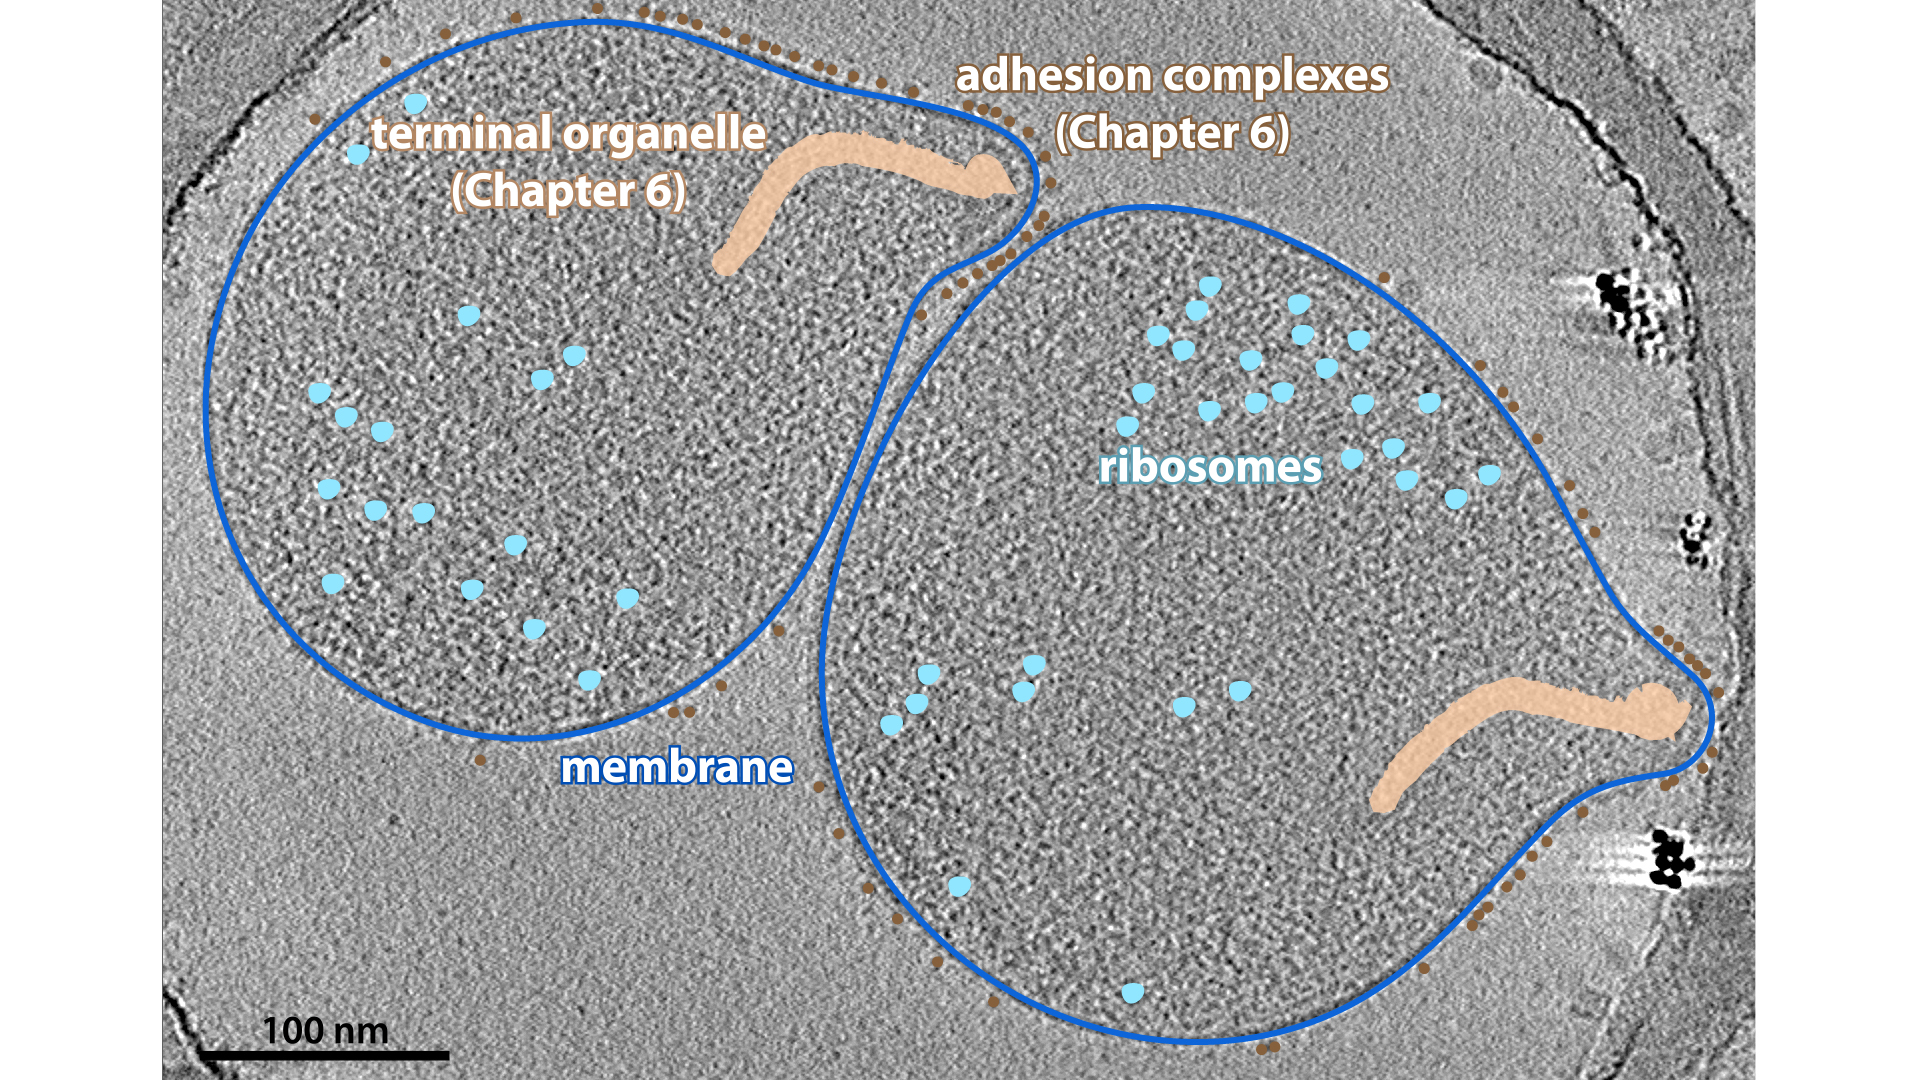
\includegraphics{img/2_1_Mgenitalium} \caption[Mycoplasma genitalium Collected by]{Mycoplasma genitalium Collected by: Gregory Henderson [10.22002/D1.1350](https://doi.org/10.22002/D1.1350)}\label{fig:unnamed-chunk-1}
\end{figure}

\hypertarget{Lipid_bilayer}{\subsection{Lipid
bilayer}\label{Lipid_bilayer}}

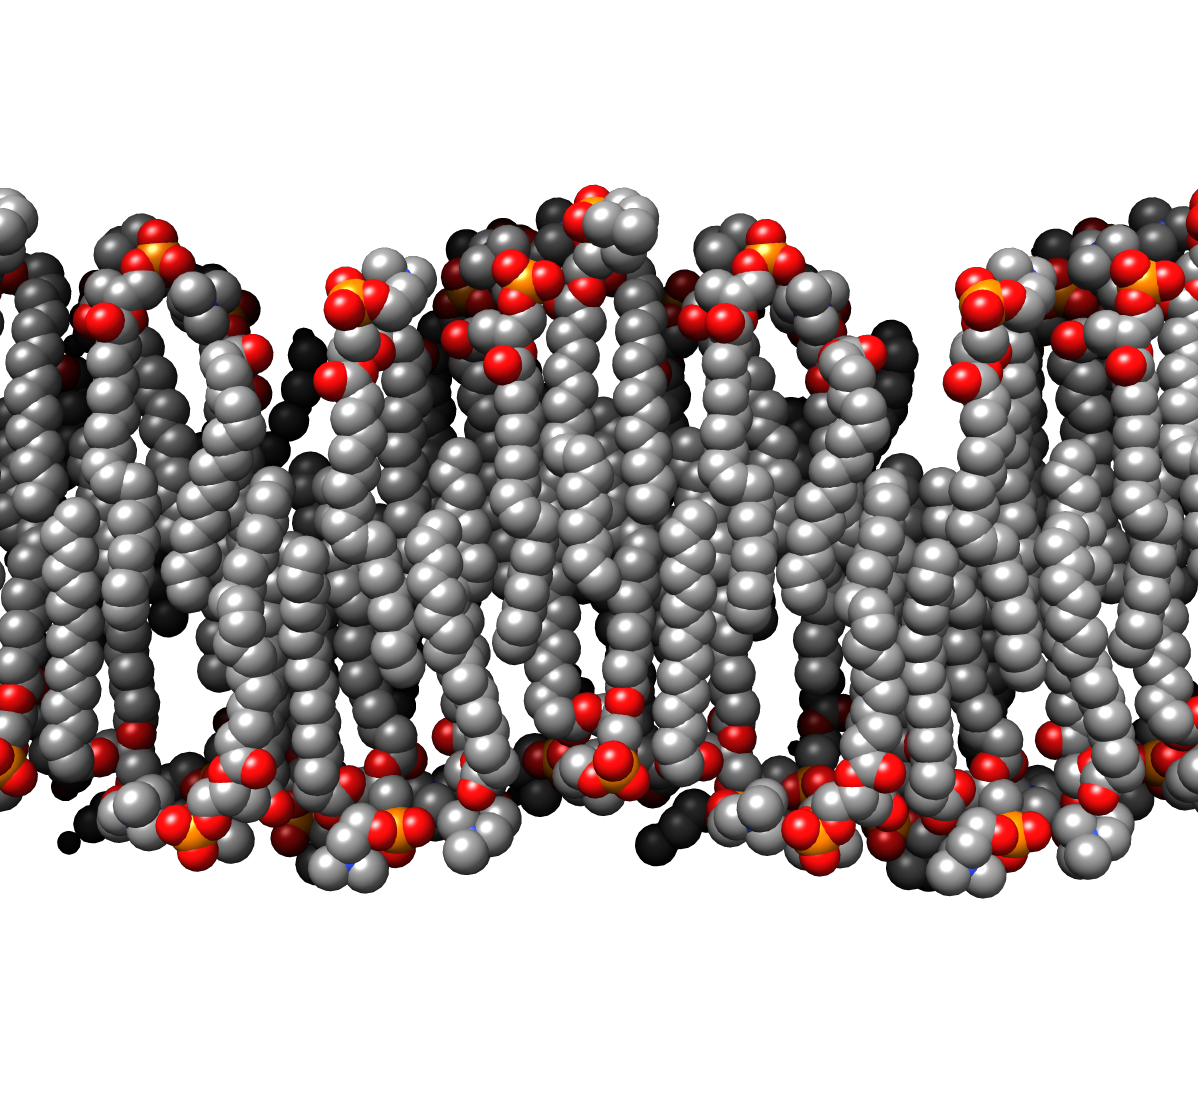
\includegraphics{img/02_schematic/2_1_1_LipidBilayer}

Lipids have a hydrophilic head (red/orange in the schematic) and
hydrophobic tails (gray); in water they spontaneously pack together
side-by-side to shield their tails from unfavorable interactions with
water, forming closed double-layered bags. Proteins with regions of
amino acids containing hydrophobic side groups embed these regions in
lipid bilayers. Other proteins are fused to lipids, tethering them to
the membrane. In fact, cells' ``lipid'' membranes actually constitute
roughly equal fractions of lipids and proteins. One key difference
between archaea and bacteria (and with them, eukaryotes) is the lipid
that makes up their membranes. Hybrid membranes containing both these
lipid types can be made artificially, and it's possible that the last
universal common ancestor of all cells on Earth contained both types,
with specialization later occurring in different lineages.

\hypertarget{ATP_synthase_and_energy_production}{\subsection{ATP
synthase and energy
production}\label{ATP_synthase_and_energy_production}}

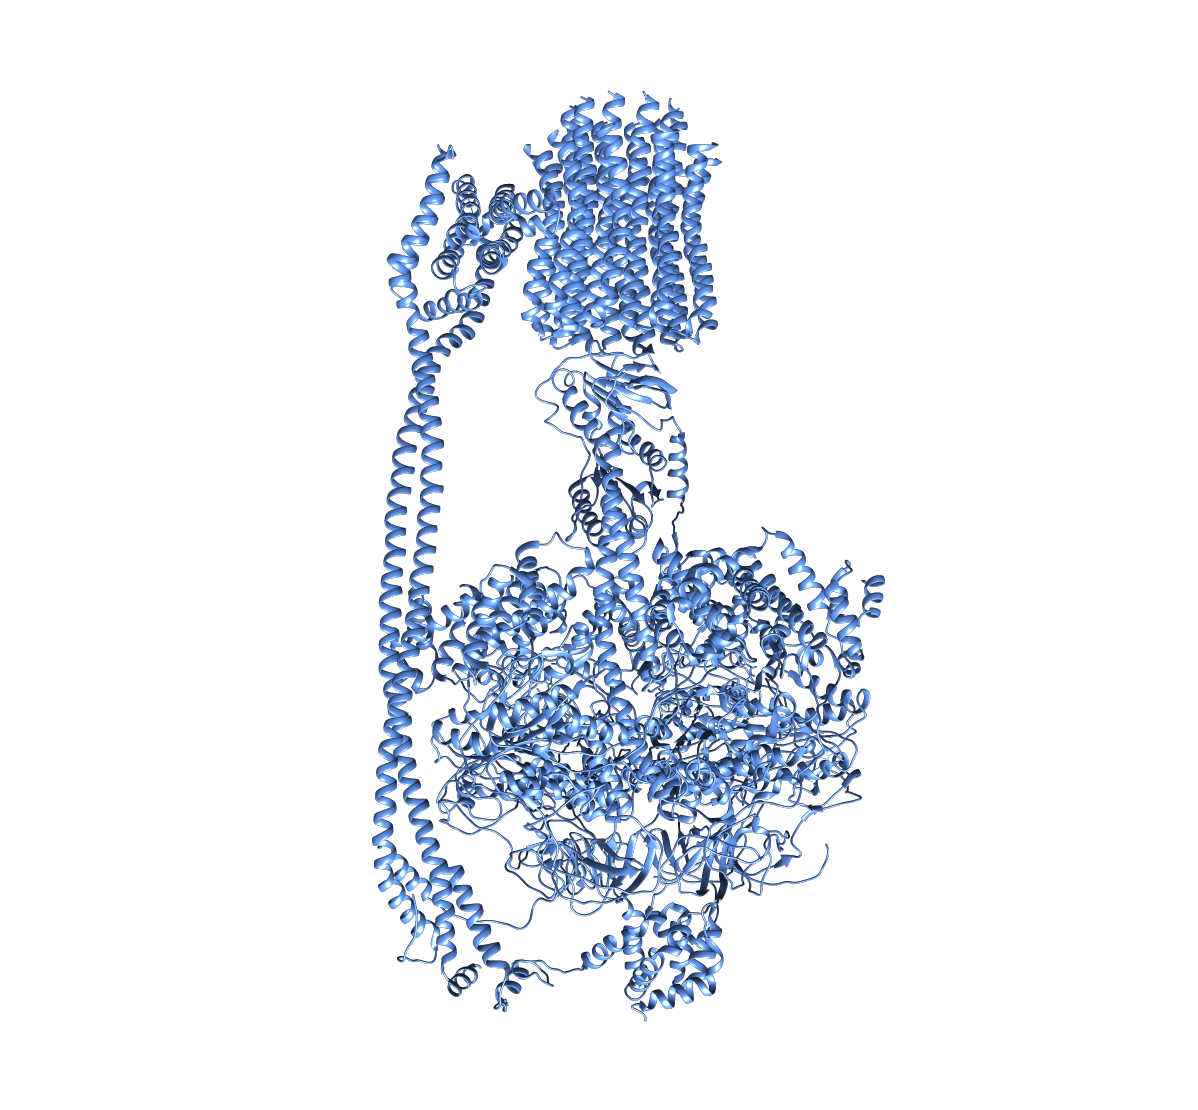
\includegraphics{img/02_schematic/2_1_2_ATPsynthase}

The chemical properties of lipids make membranes impermeable to ions and
large or hydrophilic molecules (but not to water). Cells take advantage
of this property to establish an ion gradient across the membrane, using
a chain of electron-carrying proteins in the membrane to pump protons
out of the cell. Protein complexes in the membrane called ATP synthases
(like this one from Escherichia coli) use the resulting ion potential to
generate energy. The machine provides a conduit for protons to flow down
their potential, producing a ``proton-motive force'' that spins the
machine's rotor, generating energy that is chemically stored in ATP, the
energetic currency of the cell.

\section{Listeria monocytogenes}\label{listeria-monocytogenes}

Being able to selectively move things into your cell enables it to do
some powerful things. It also poses a structural problem, though.
Remember that water can pass freely through the membrane, which means
that increasing the solute concentration inside relative to the
environment will cause water to rush in as well, introducing a pressure
(known as turgor pressure) on the membrane. Lipid bilayers, though, are
unable to withstand much pressure. If your cell lives exclusively in a
consistent, and fairly high-osmolarity, environment (like our bodies, in
the case of the Mycoplasma genitalium you just saw), it can balance
internal and external osmolarity to minimize turgor pressure on the
membrane. But most cells experience much more variable environments. How
can you keep your cell from bursting in such conditions?

You'll probably want to add some rigid scaffolding outside the membrane
to buttress it against turgor pressure. Nearly all bacteria do this
using a material called peptidoglycan: long stiff polymers of glycan
sugars crosslinked by short peptides into a chain-mail-like mesh. The
full scaffold of this material surrounding the cell is called its
sacculus, or cell wall. Some archaea also have cell walls, made of a
molecule similar to peptidoglycan, but chemically distinct. Most
archaea, though, rely on a different structure for support, as you'll
see later in this chapter.

In monoderm bacteria like this Listeria monocytogenes, the cell wall is
significantly thicker than the membrane. It comprises several layers of
peptidoglycan, which can't be seen individually at the resolution of
this image, so the cell wall appears as a uniformly textured layer
\protect\hyperlink{Peptidoglycan_architecture}{More: Peptidoglycan
architecture}. It's still a mystery how large molecules can pass through
this dense layer on their way to and from the cell. Not all bacterial
cell walls are chemically identical \protect\hyperlink{}{More:
Methanobacterium formicicum}. And in some conditions, cells can lose
their walls \protect\hyperlink{L-form_bacteria}{Schematic -- L-form
bacteria}.

\begin{figure}
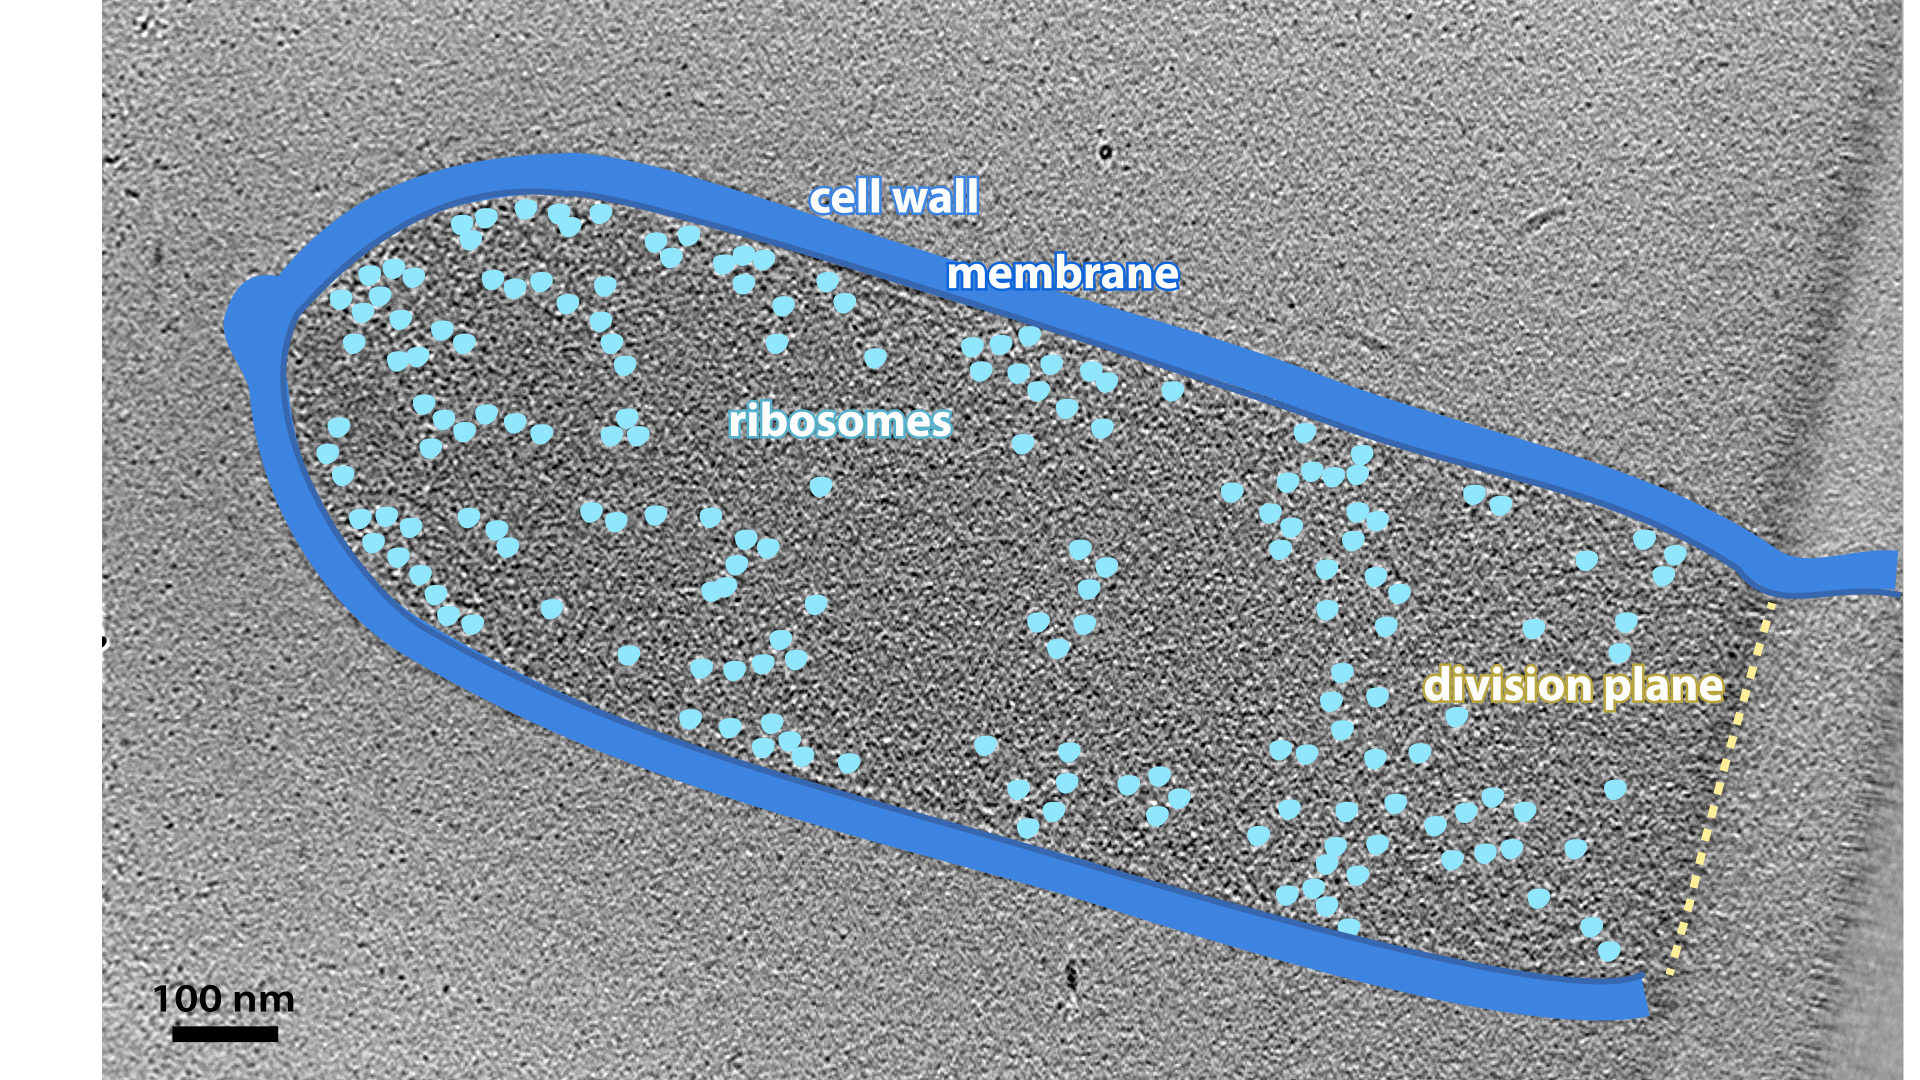
\includegraphics{img/2_2_Lmonocytogenes} \caption[Listeria monocytogenes Collected by]{Listeria monocytogenes Collected by: Ariane Briegel [10.22002/D1.1351](https://doi.org/10.22002/D1.1351)}\label{fig:unnamed-chunk-4}
\end{figure}

\hypertarget{Peptidoglycan_architecture}{\subsection{Bacillus
subtilis}\label{Peptidoglycan_architecture}}

The sacculus is so robust that it persists even after cells are lysed
and their other components digested. This sacculus isolated from a
Bacillus subtilis cell has retained its shape, simply flattening with
the release of contents and pressure from inside. By observing how these
purified sacculi rip and curl, we can infer something about the
architecture of the cell wall; we think that the long glycan strands are
oriented in hoops circling the short axis of the cylindrical cell and
the short peptide crosslinks are more or less aligned with the long
axis.

\begin{figure}
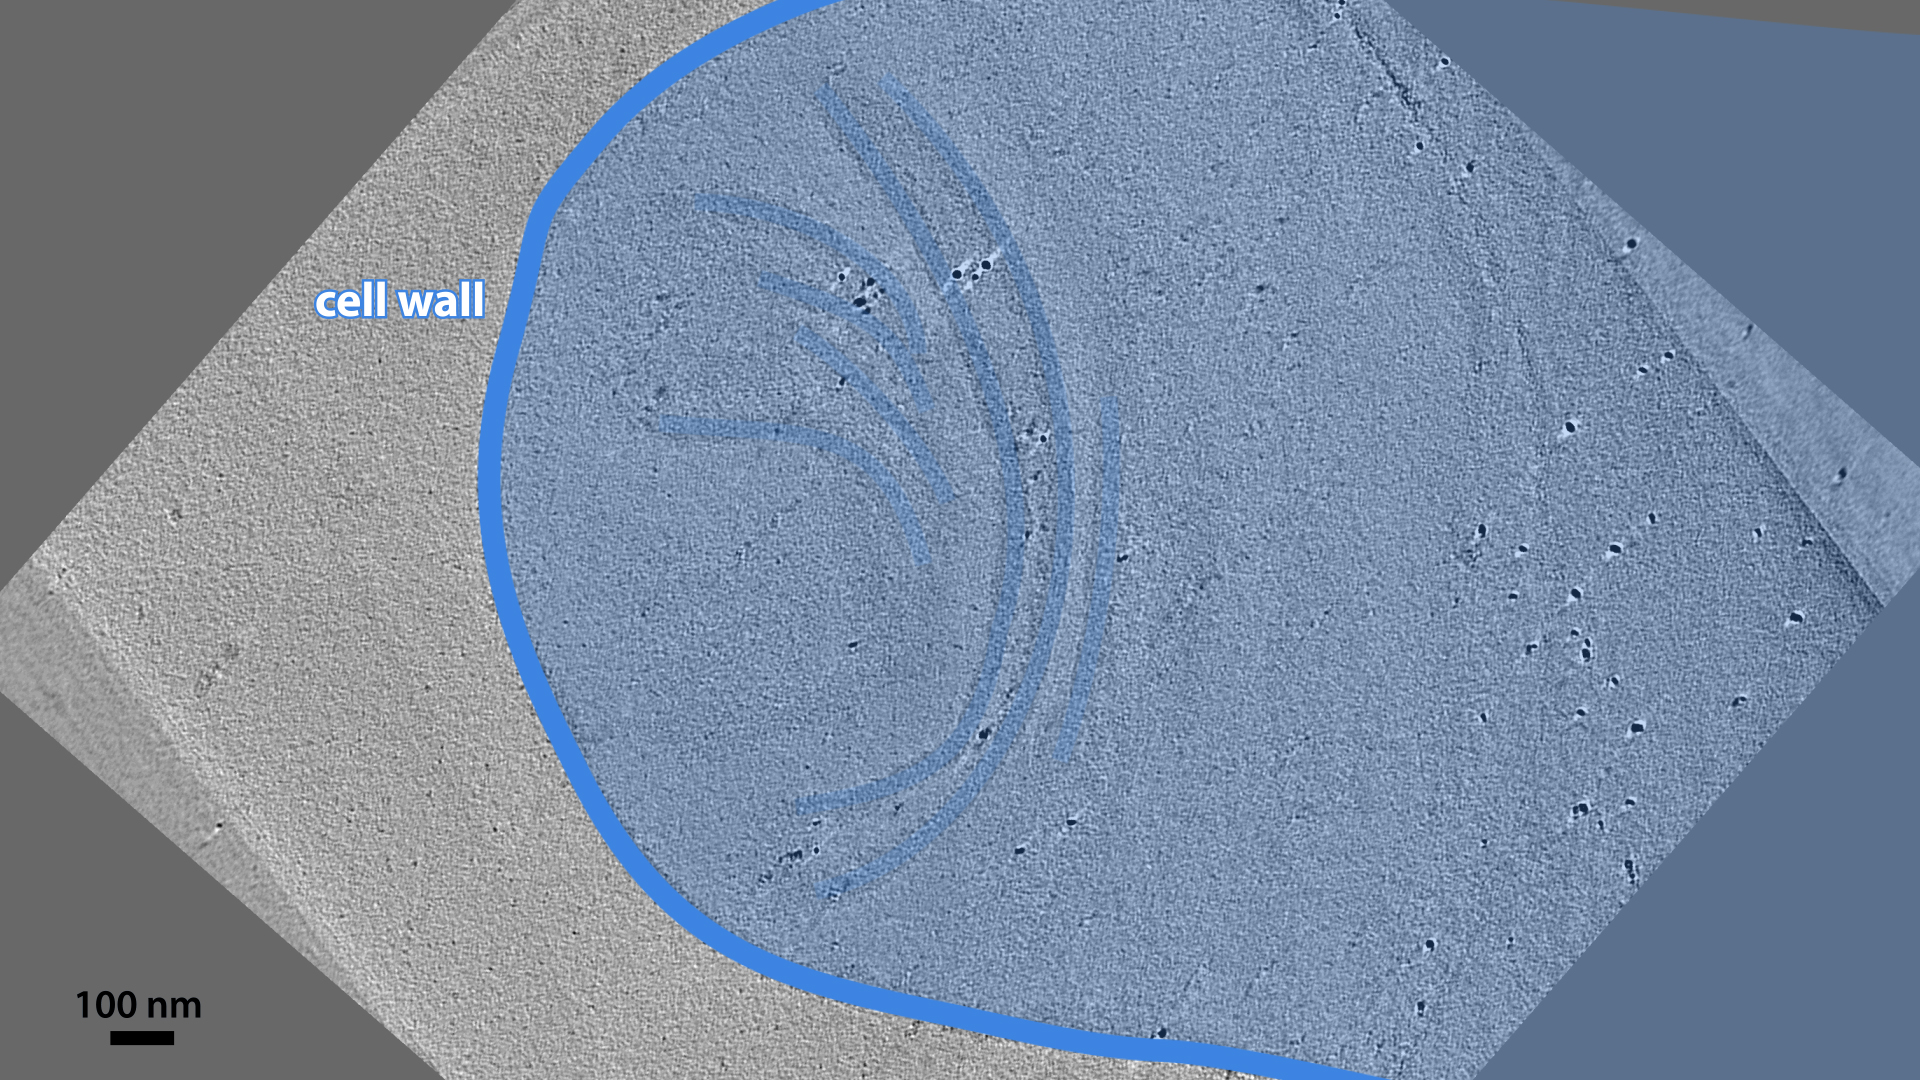
\includegraphics{img/2_2a_Bsubtilis} \caption[Bacillus subtilis Collected by]{Bacillus subtilis Collected by: Morgan Beeby [10.22002/D1.1360](https://doi.org/10.22002/D1.1360)}\label{fig:unnamed-chunk-5}
\end{figure}

\hypertarget{L-form_bacteria}{\subsection{L-form
bacteria}\label{L-form_bacteria}}

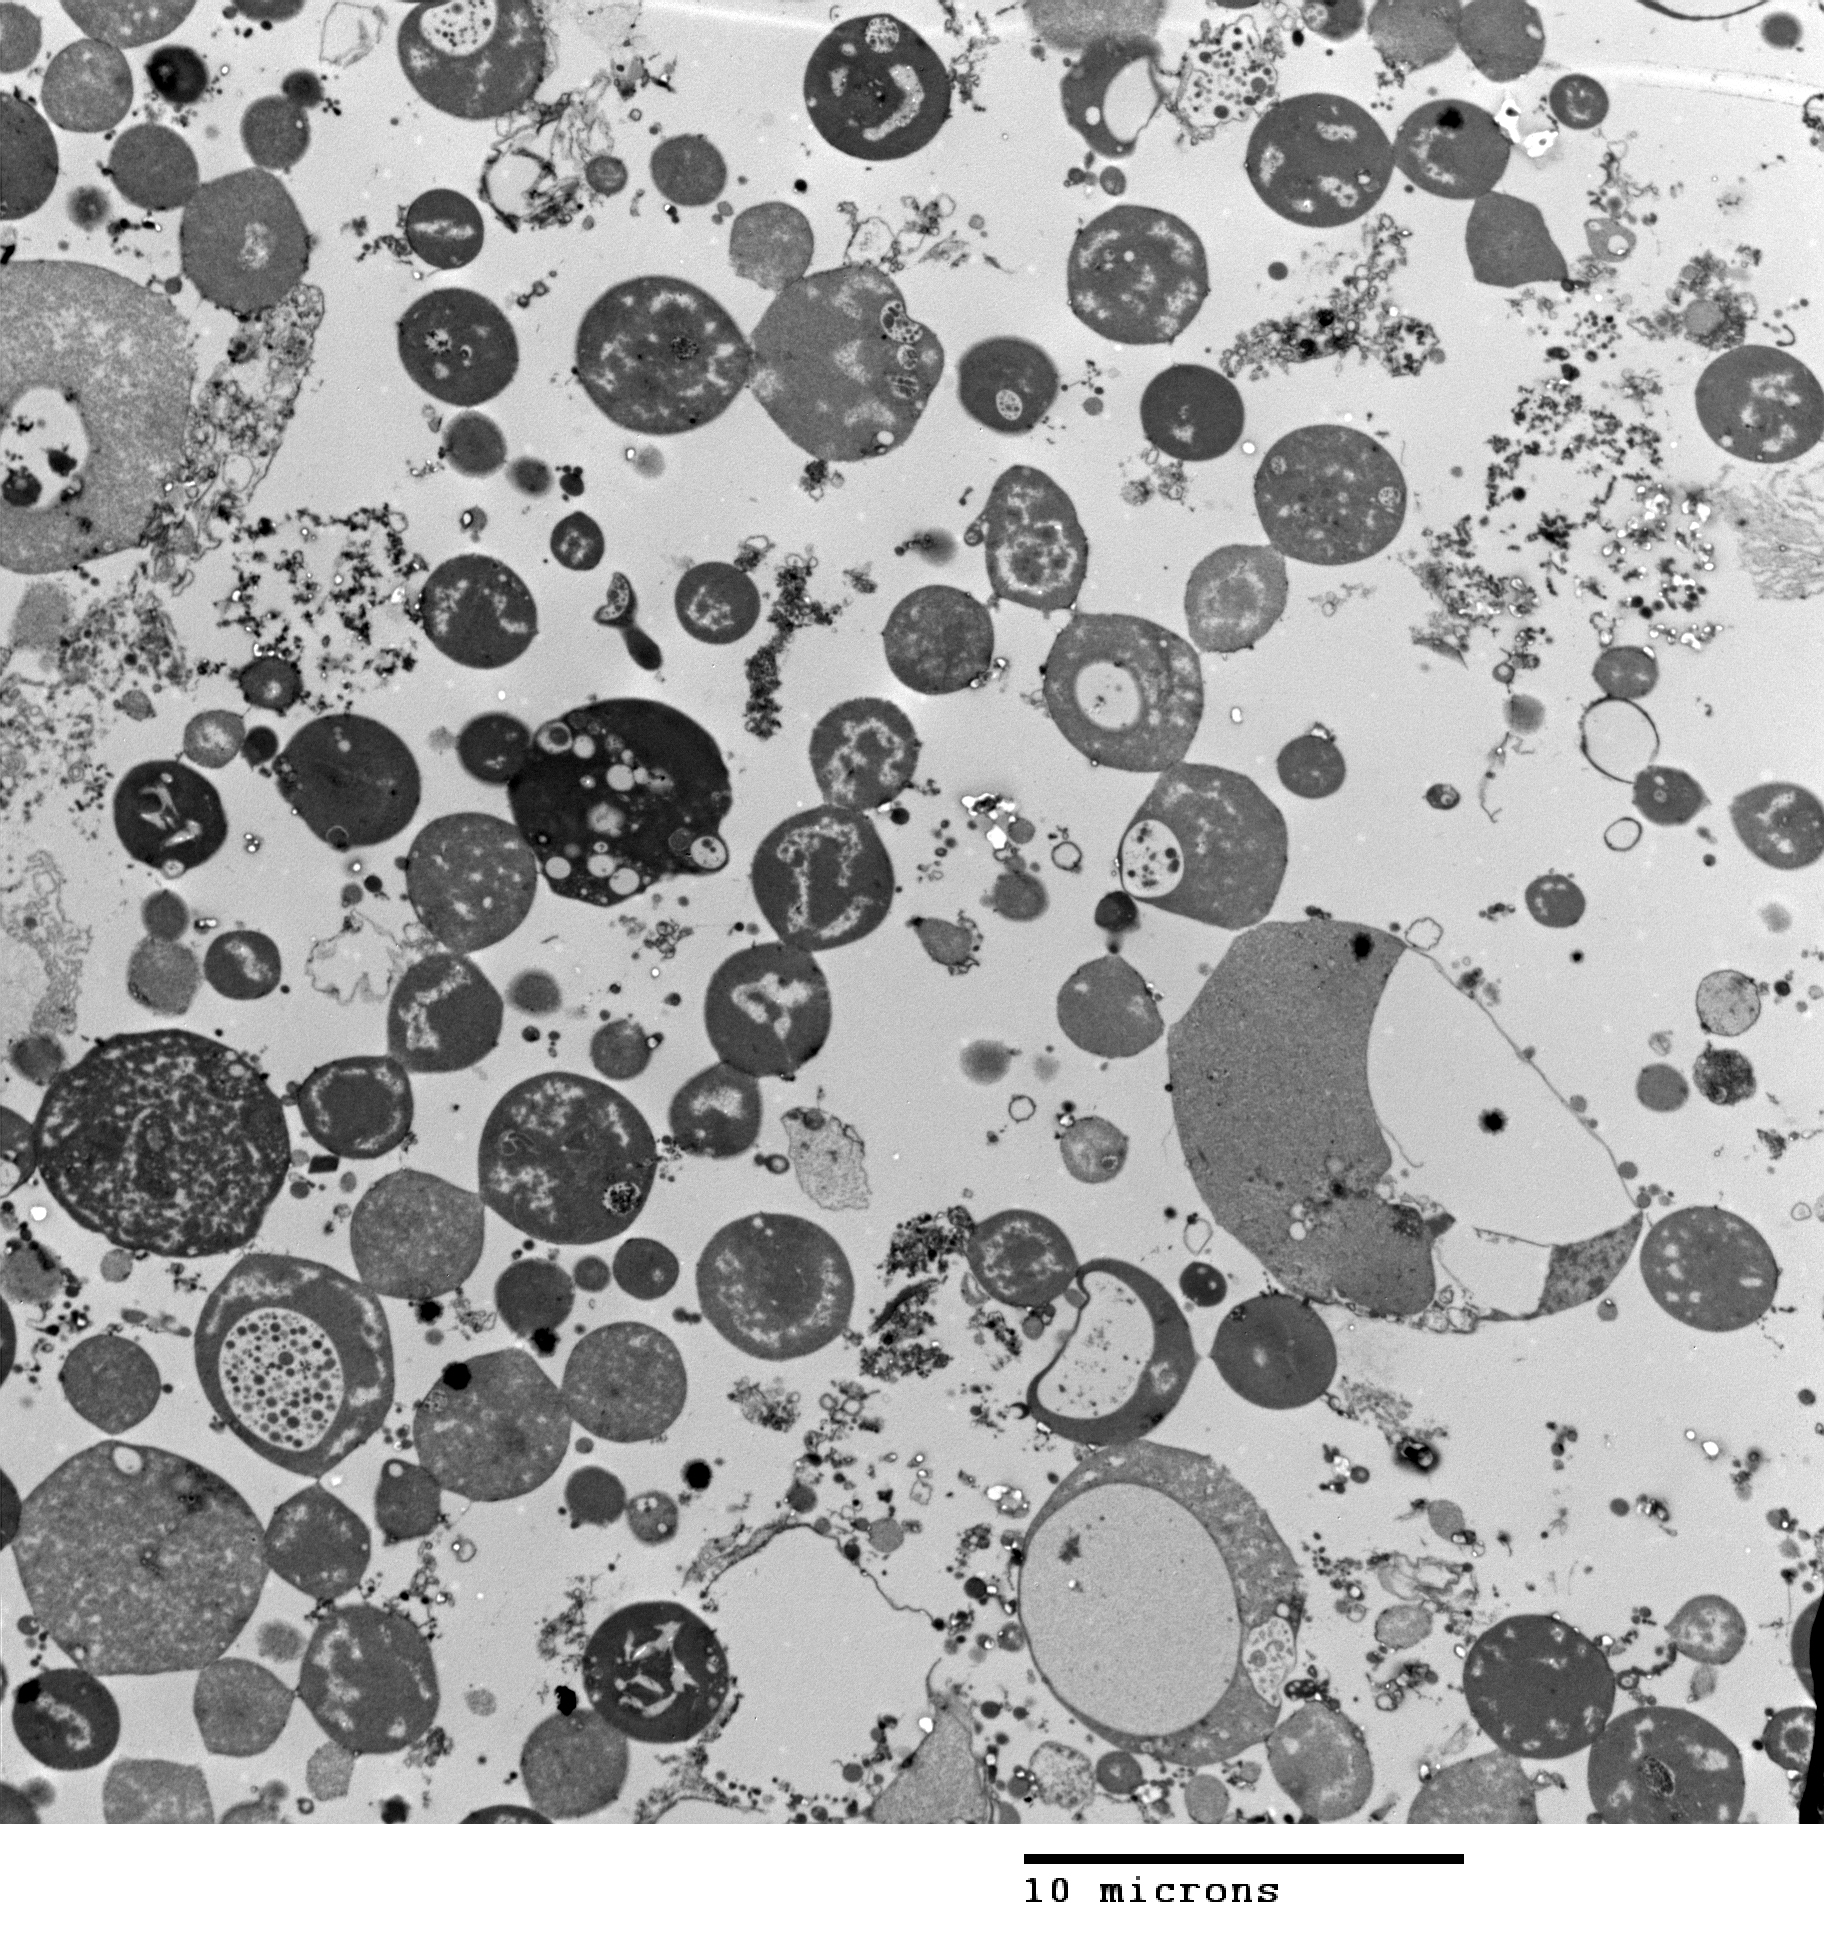
\includegraphics{img/02_schematic/2_2_1_L_form_bacteria}

There is no universal adaptation in Nature; advantages in one
environment can become liabilities in another. This concept is
exemplified by an adaptation of some bacteria which lose their cell
walls in certain conditions, such as in the presence of antibiotics (the
cell wall is a common target of antibiotics). This state is called the
L-form (named for the Lister Institute where it were discovered). As you
can see in these Bacillus subtilis, cells in this state are pleomorphic,
exhibiting a variety of sizes and shapes. As you would expect, L-form
cells are more sensitive to environmental conditions. In the lab,
they're protected from lysis by increasing the osmotic pressure of the
environment, for instance by adding sucrose. The environment in your
body, though, would have the same effect, as we discussed for Mycoplasma
genitalium. L-form bacteria are interesting for many reasons (including
human health), one of which is that they give us a fascinating window
into how early cells -- prior to the evolution of the cell wall -- might
have looked and behaved.

\section{Cupriavidus necator}\label{cupriavidus-necator}

Why stop at one membrane, though? Think about how the bacteria you've
just seen compare with eukaryotic cells. The eukaryotic cells are much
larger (maybe 100-1,000 times larger in volume), and they contain many
internal membranes that form specialized subcompartments, like the
nucleus and mitochondria. Bacteria and archaea don't have membrane-bound
organelles inside, but in fact many bacteria do create an additional
compartment outside the cell with another, outer, membrane. These
bacteria, like the Cupriavidus necator cell you see here, are called
diderms (``double skin''). The extra compartment between their membranes
is known as the periplasm (``mold between''). This antechamber contains
a unique subset of proteins, many of which function in escorting things
into and out of the main cell, as you'll see in later chapters.

Compared to the inner membrane, the outer membrane has some unique
properties! It is more permeable and not proton-tight (so it can't be
used to generate ATP). It is often asymmetric, with a different
composition of lipids and proteins in each of the two leaflets. The
outer membrane is anchored to the sacculus
\protect\hyperlink{Brauns_lipoprotein}{Schematic -- Braun's
lipoprotein}. And the sacculus itself is different. Rather than
containing many layers of peptidoglycan like in the Listeria
monocytogenes cell you just saw, the diderm sacculus consists largely of
a single-layered peptidoglycan mesh
\protect\hyperlink{Diderm_sacculus_architecture}{More: Diderm sacculus
architecture}, which you can see here as a thin line in the periplasm.
This difference in the sacculus enables a well-known bacterial
classification system: the Gram stain, which binds peptidoglycan.
Gram-positive cells, typically monoderm, contain much more peptidoglycan
than Gram-negative cells, which are typically diderm. Thinking about
this thin defense against turgor pressure underscores a major challenge
for cell growth. To insert new material, existing bonds in the sacculus
must be broken, without bursting the cell in the process
\protect\hyperlink{Sacculus_remodeling}{Schematic -- Sacculus
remodeling}.

\begin{figure}
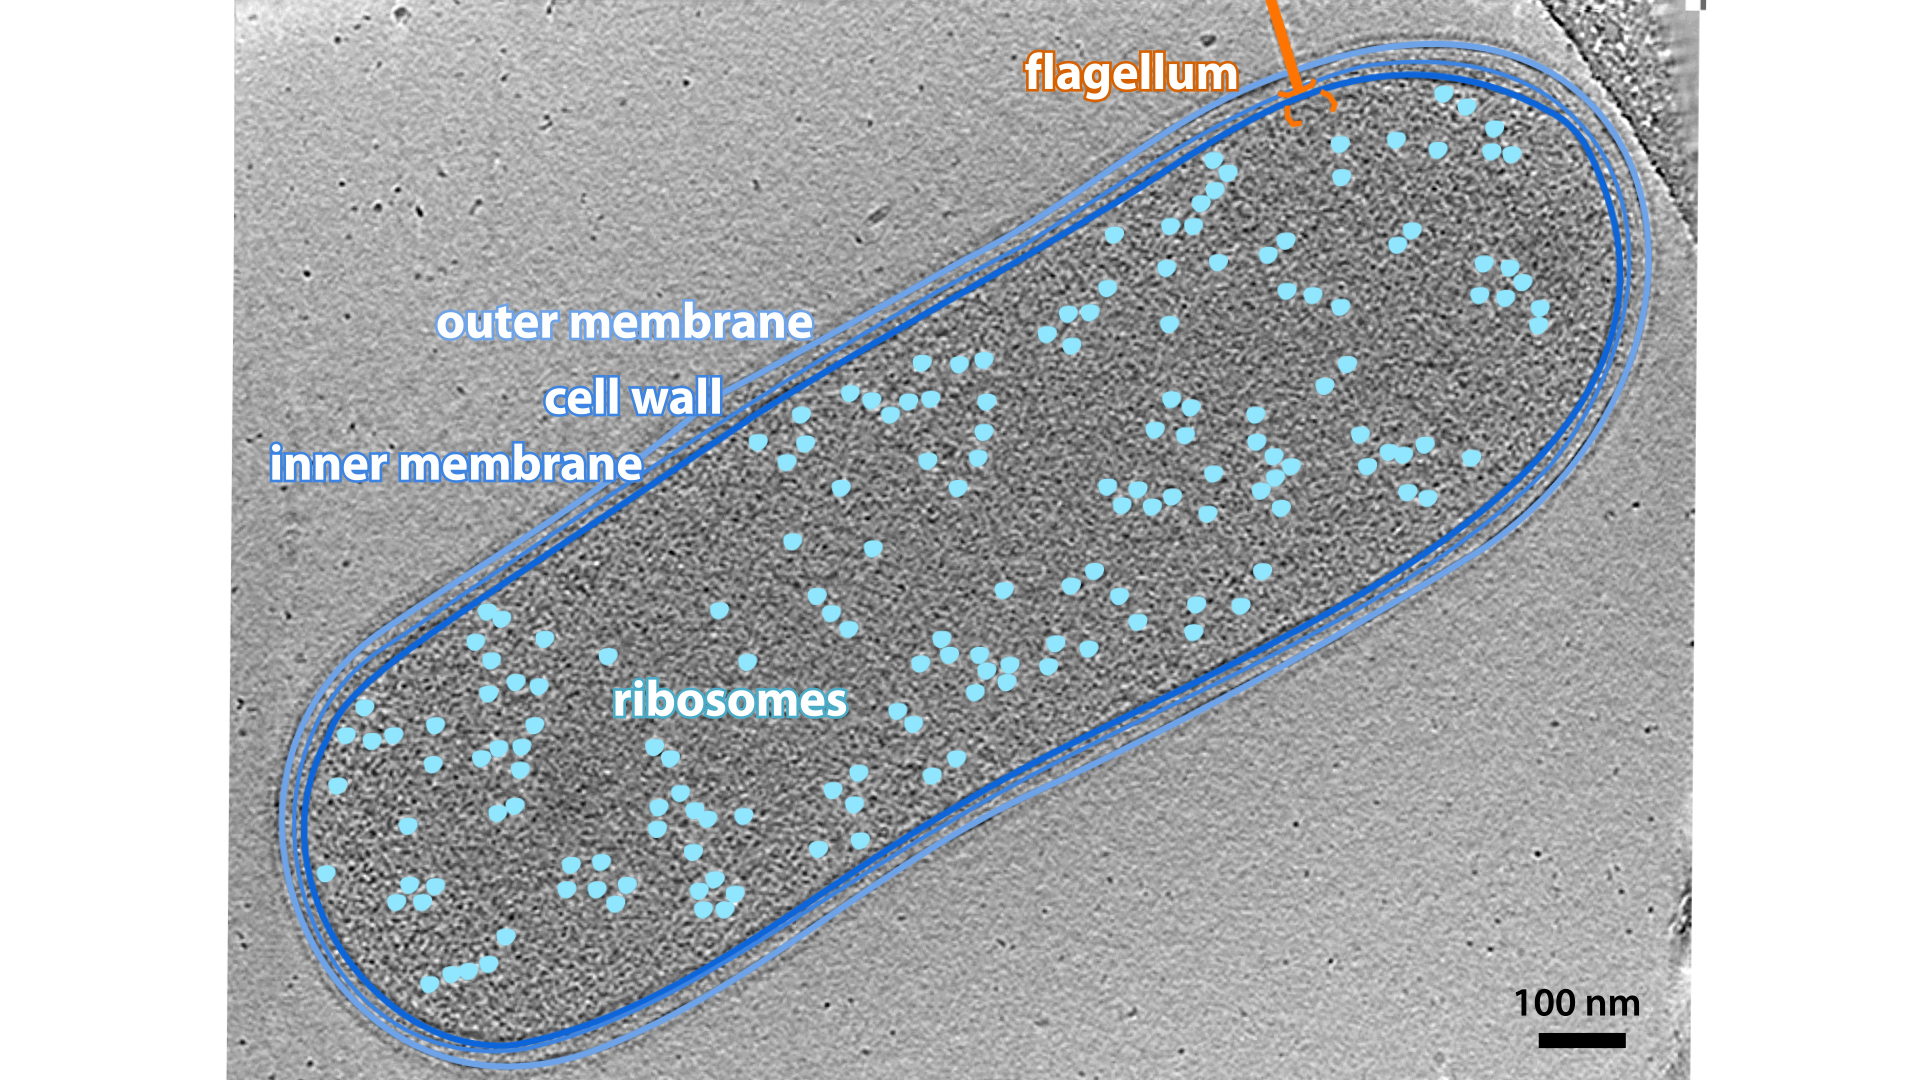
\includegraphics{img/2_3_Hcrunogenus} \caption[Hydrogenovibrio crunogenus Collected by]{Hydrogenovibrio crunogenus Collected by: Cristina Iancu [10.22002/D1.1352](https://doi.org/10.22002/D1.1352)}\label{fig:unnamed-chunk-7}
\end{figure}

\hypertarget{Brauns_lipoprotein}{\subsection{Braun's
lipoprotein}\label{Brauns_lipoprotein}}

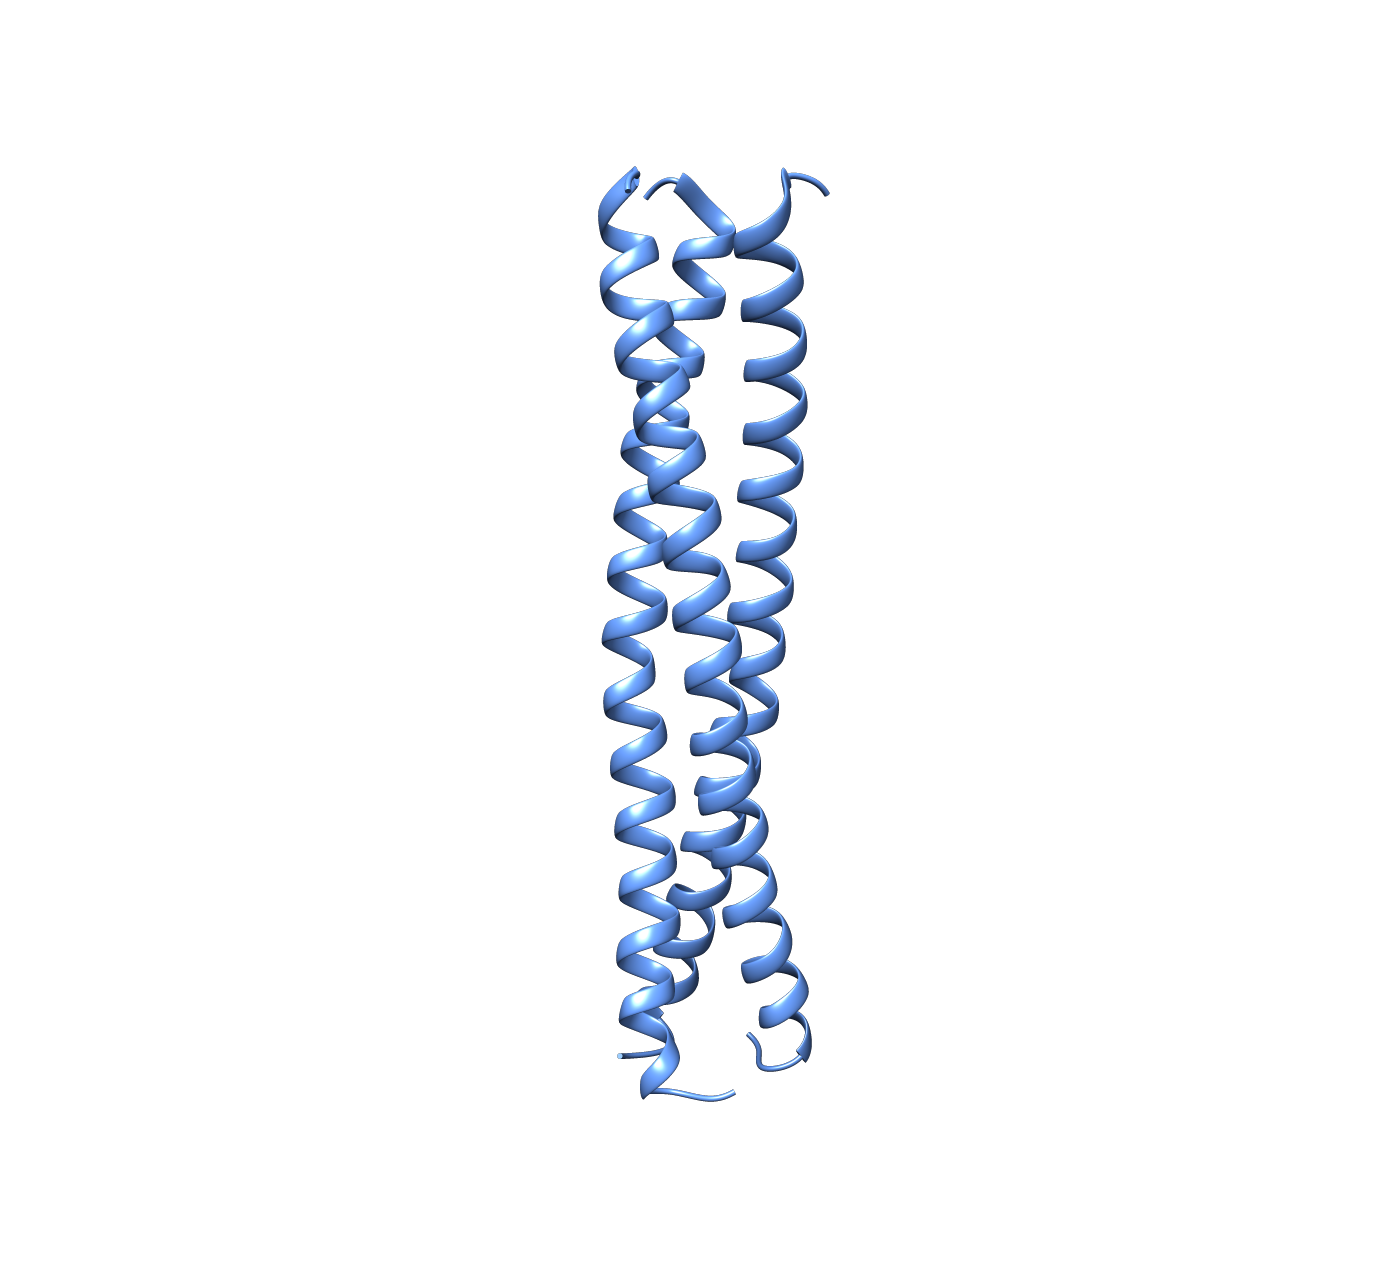
\includegraphics{img/02_schematic/2_3_1_BLP}

Lipoproteins are hybrid molecules, formed by covalently linked lipid and
protein pieces. The lipid allows them to embed into a membrane,
tethering the attached protein to function nearby. Braun's lipoprotein,
which is one of the most abundant molecules in the outer membrane of
cells like Escherichia coli, uses its tethered protein portion to bind
the peptidoglycan cell wall, creating a link between the outer membrane
and the cell wall (adding up, for a typical E. coli cell, to about
100,000 links). These links determine the distance between these two
components. Not all diderms use Braun's lipoprotein, though, and some
bacteria have notably labile outer membranes \protect\hyperlink{}{More:
Outer membrane lability}.

\hypertarget{Diderm_sacculus_architecture}{\subsection{Escherichia
coli}\label{Diderm_sacculus_architecture}}

Compare this diderm sacculus purified from Escherichia coli to the
monoderm sacculus on the last page. Since this one is thinner; we can
make out more details. Instead of inferring how the glycan strands are
oriented, we can now see them running around the circumference of the
cell. The main difference between the two types of sacculi seems to be
whether they have largely a single layer of peptidoglycan (diderm) or
many layers (monoderm). So even though the two cell walls look
different, their architecture is fundamentally the same. In some
circumstances, cells can even switch between the two forms, as you'll
see in Chapter 7.

\begin{figure}
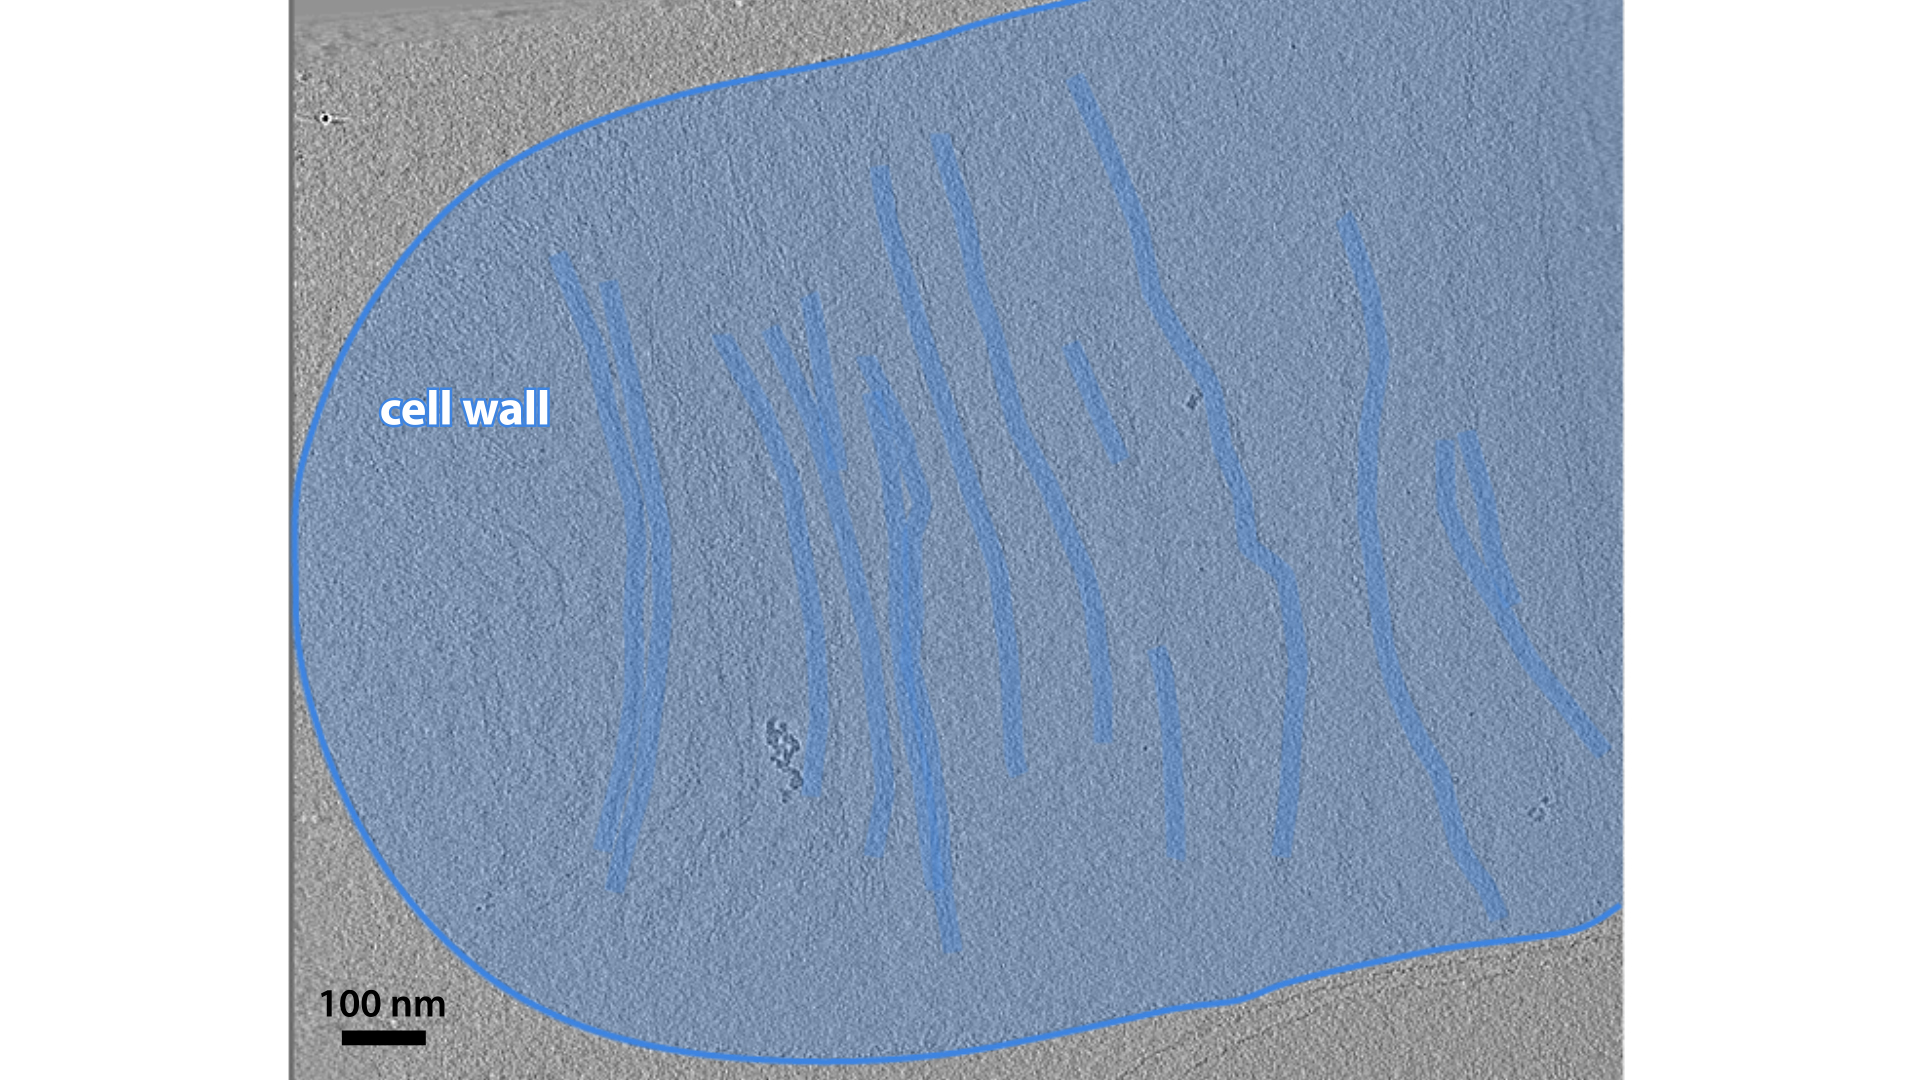
\includegraphics{img/2_3a_Ecoli} \caption[Escherichia coli Collected by]{Escherichia coli Collected by: Lu Gan [10.22002/D1.1362](https://doi.org/10.22002/D1.1362)}\label{fig:unnamed-chunk-9}
\end{figure}

\hypertarget{Sacculus_remodeling}{\subsection{Sacculus
remodeling}\label{Sacculus_remodeling}}

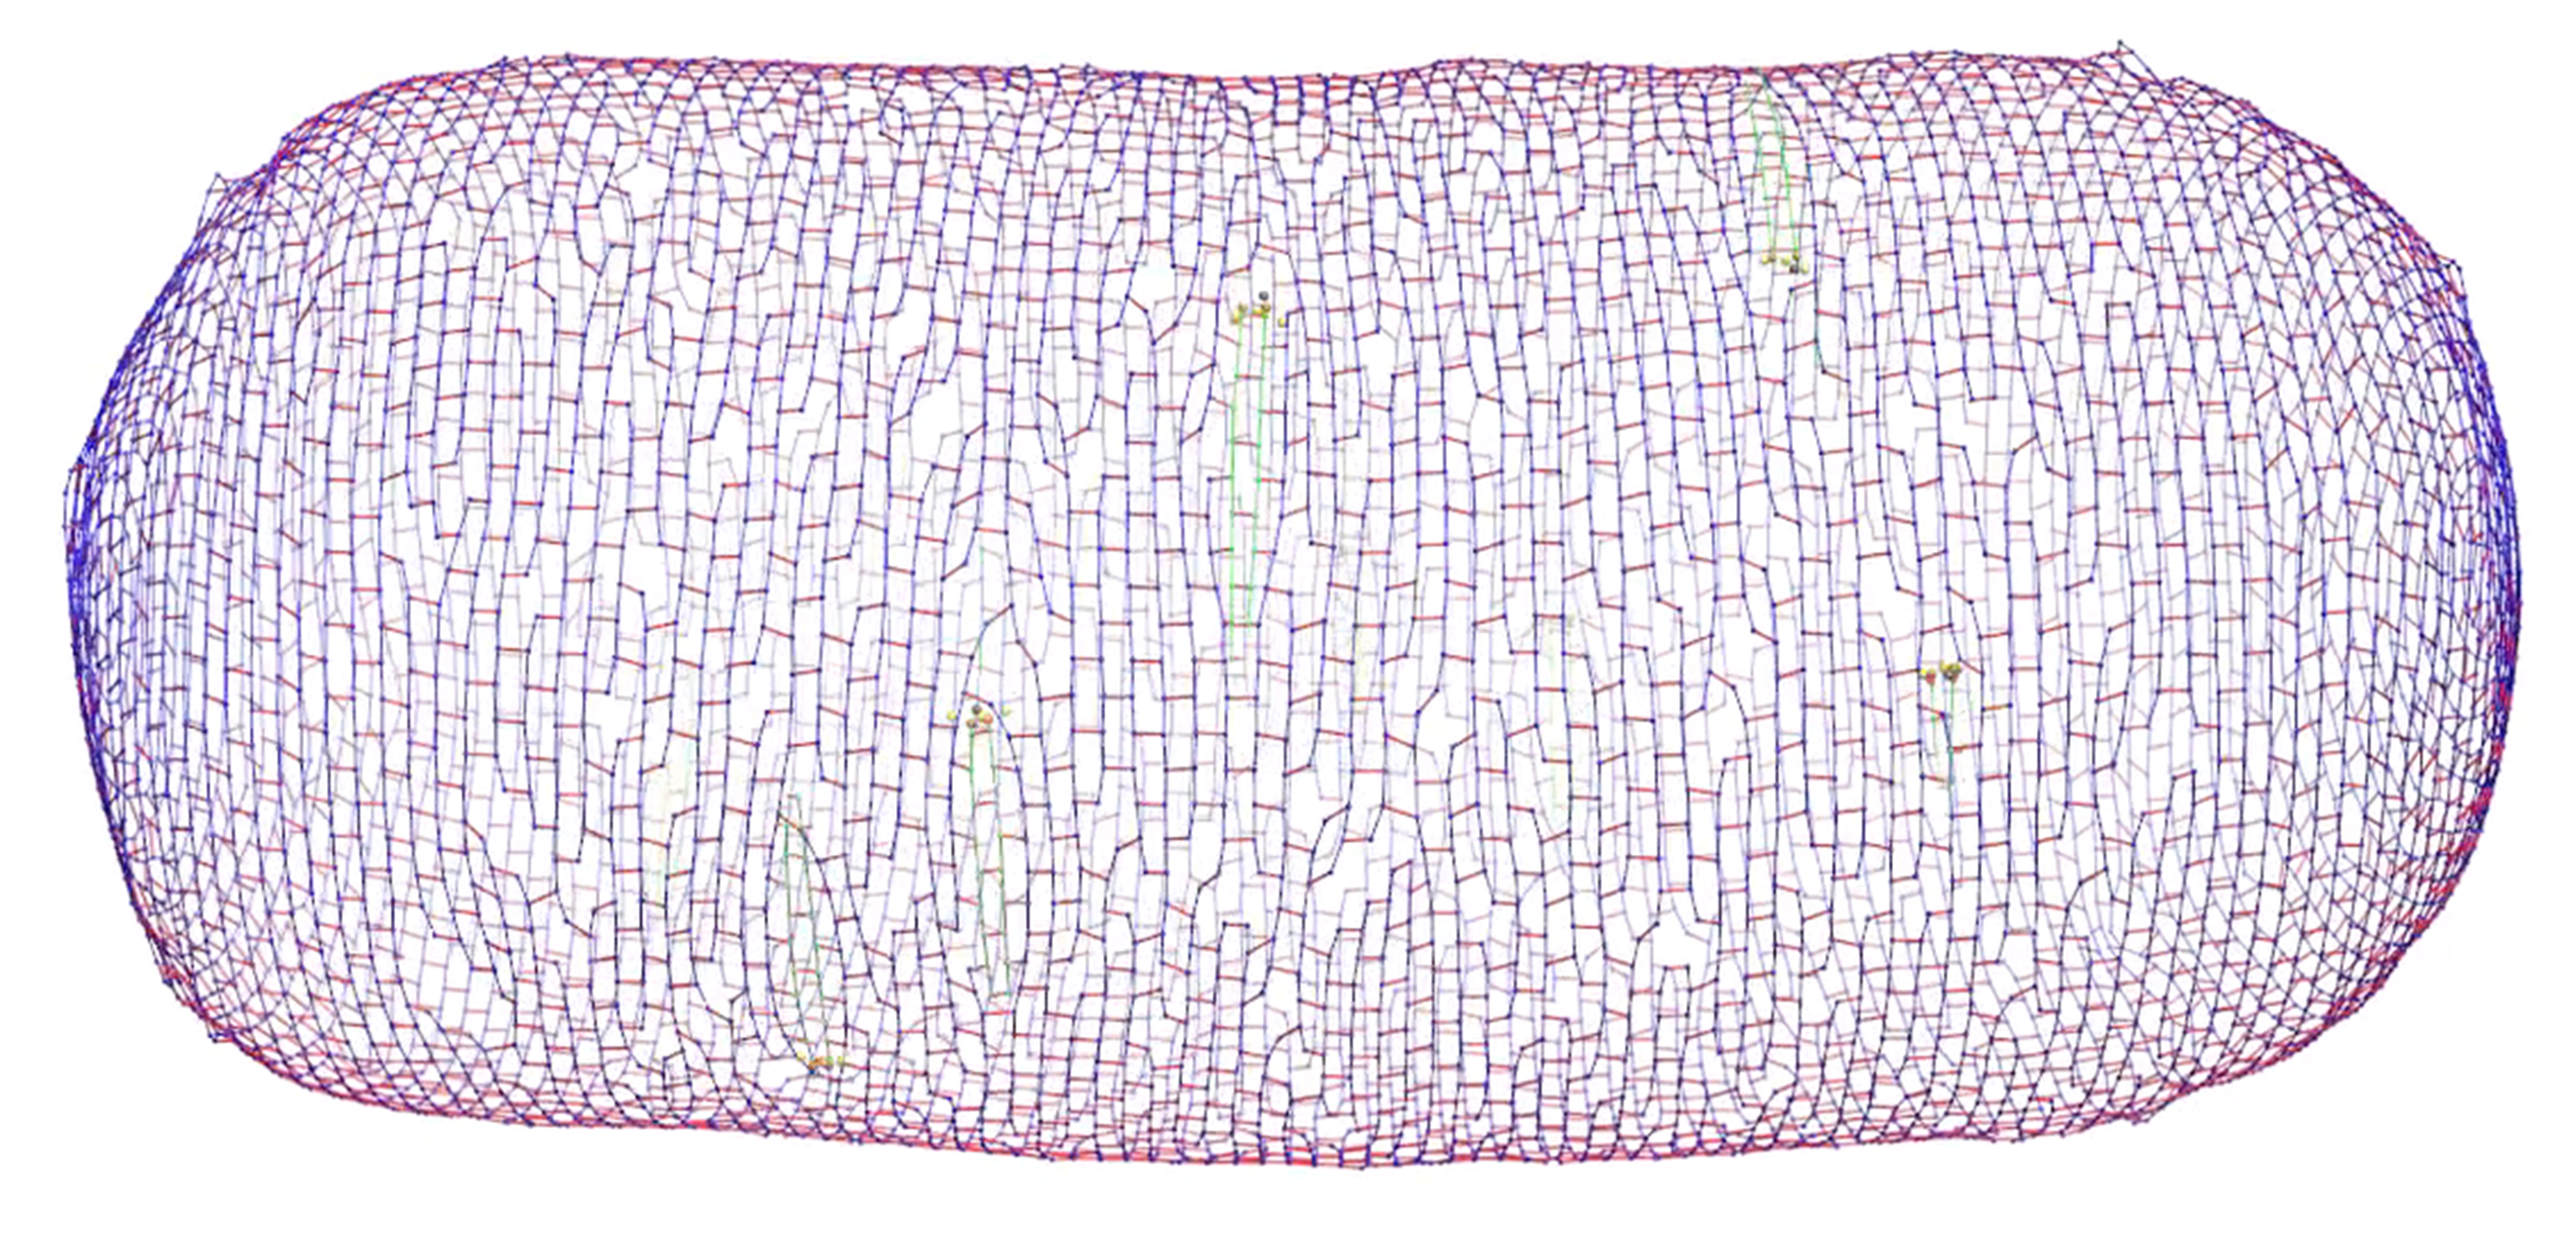
\includegraphics{img/02_schematic/2_3_2_SacculusRemodeling}

Encasing your cell in a rigid scaffold presents a problem: how can it
grow? It's easy to make membranes larger simply by adding more lipids.
But to add more peptidoglycan strands, they have to be linked into the
existing network, which means breaking existing links to accommodate
them. In fact, cells remodel their sacculi with the tools you'd expect:
an enzyme that links glycan sugars into strands, an enzyme that links
strands together with peptide bonds, and an enzyme that cuts these
peptide links. Remember, though, that your cell, with its solute-rich
interior, has a turgor pressure pushing outward with a force of maybe 3
atmospheres, equivalent to what we would feel at a depth of 20 meters in
the ocean. This is more than enough to lyse an exposed bacterial
membrane. So these tools must be used carefully to ensure that the cell
doesn't burst. We're still figuring out exactly how this works, with
help from computer simulations like this one. Here you see a model of an
Escherichia coli sacculus being enlarged using the three enzyme tools we
just described. This simulation was run to test whether just having the
tools function in a complex rather than separately might give enough
coordination for smooth, safe growth. (The answer was yes.)

More: Diderm archaea Nearly all diderm cells are bacteria. Not all,
though. As you see here, Ignicoccus hospitalis, an archaeon, has an
outer membrane that appears very loosely associated with the cell,
forming an extra large periplasm. You can see membrane-bound vesicles
shuttling cargo across this vast space (more about vesicles on the next
page). Interestingly, this is also an exception to the rule that the
inner membrane of diderms is ``energized'' (proton-tight). In I.
hospitalis, it is the outer membrane that contains the ATP synthases.
These unusual characteristics suggest a symbiotic origin for this
species; perhaps its ancestor used to live inside a host cell, which was
eventually reduced to a mere membrane.

\section{Borrelia burgdorferi}\label{borrelia-burgdorferi}

What else can you do with an extra membrane? Since membranes make
excellent containers for molecules, why not get into the shipping
business? In the coming chapters (especially Chapter 8), you'll see some
of the ways that cells interact with each other and their environment.
For diderm bacteria, many of these interactions are made possible by
outer membrane vesicles (``little bladders'')--self-contained pockets
budded off the membrane. The vesicles may carry cargo of antibiotics to
inhibit competitors' growth, or toxins to lyse neighboring cells. Or
enzymes to digest those lysed remains into nutrients that your cell can
easily take up as food. Alternatively, they may carry emergency kits
(first aid and survival factors) for other members of a community
biofilm. The appearance of these vesicles varies as much as their
contents \protect\hyperlink{Vesicle_morphologies}{More: Vesicle
morphologies}. They are usually spherical, of a consistent size, and
often come off the cell at one or a few sites, forming chains, as you
can see in this Borrelia burgdorferi cell.

Not all diderms produce outer membrane vesicles, and even for the ones
that do, we still don't know exactly how they do it. Maybe it happens
spontaneously due to the physics of lipids and proteins in a certain
configuration. Or maybe there's a dedicated protein machine in the
membrane, blowing bubbles. Some archaea (monoderms) also produce
membrane vesicles. They're less studied than their bacterial
counterparts, but likely serve similar roles in metabolism and community
interactions.

\begin{figure}
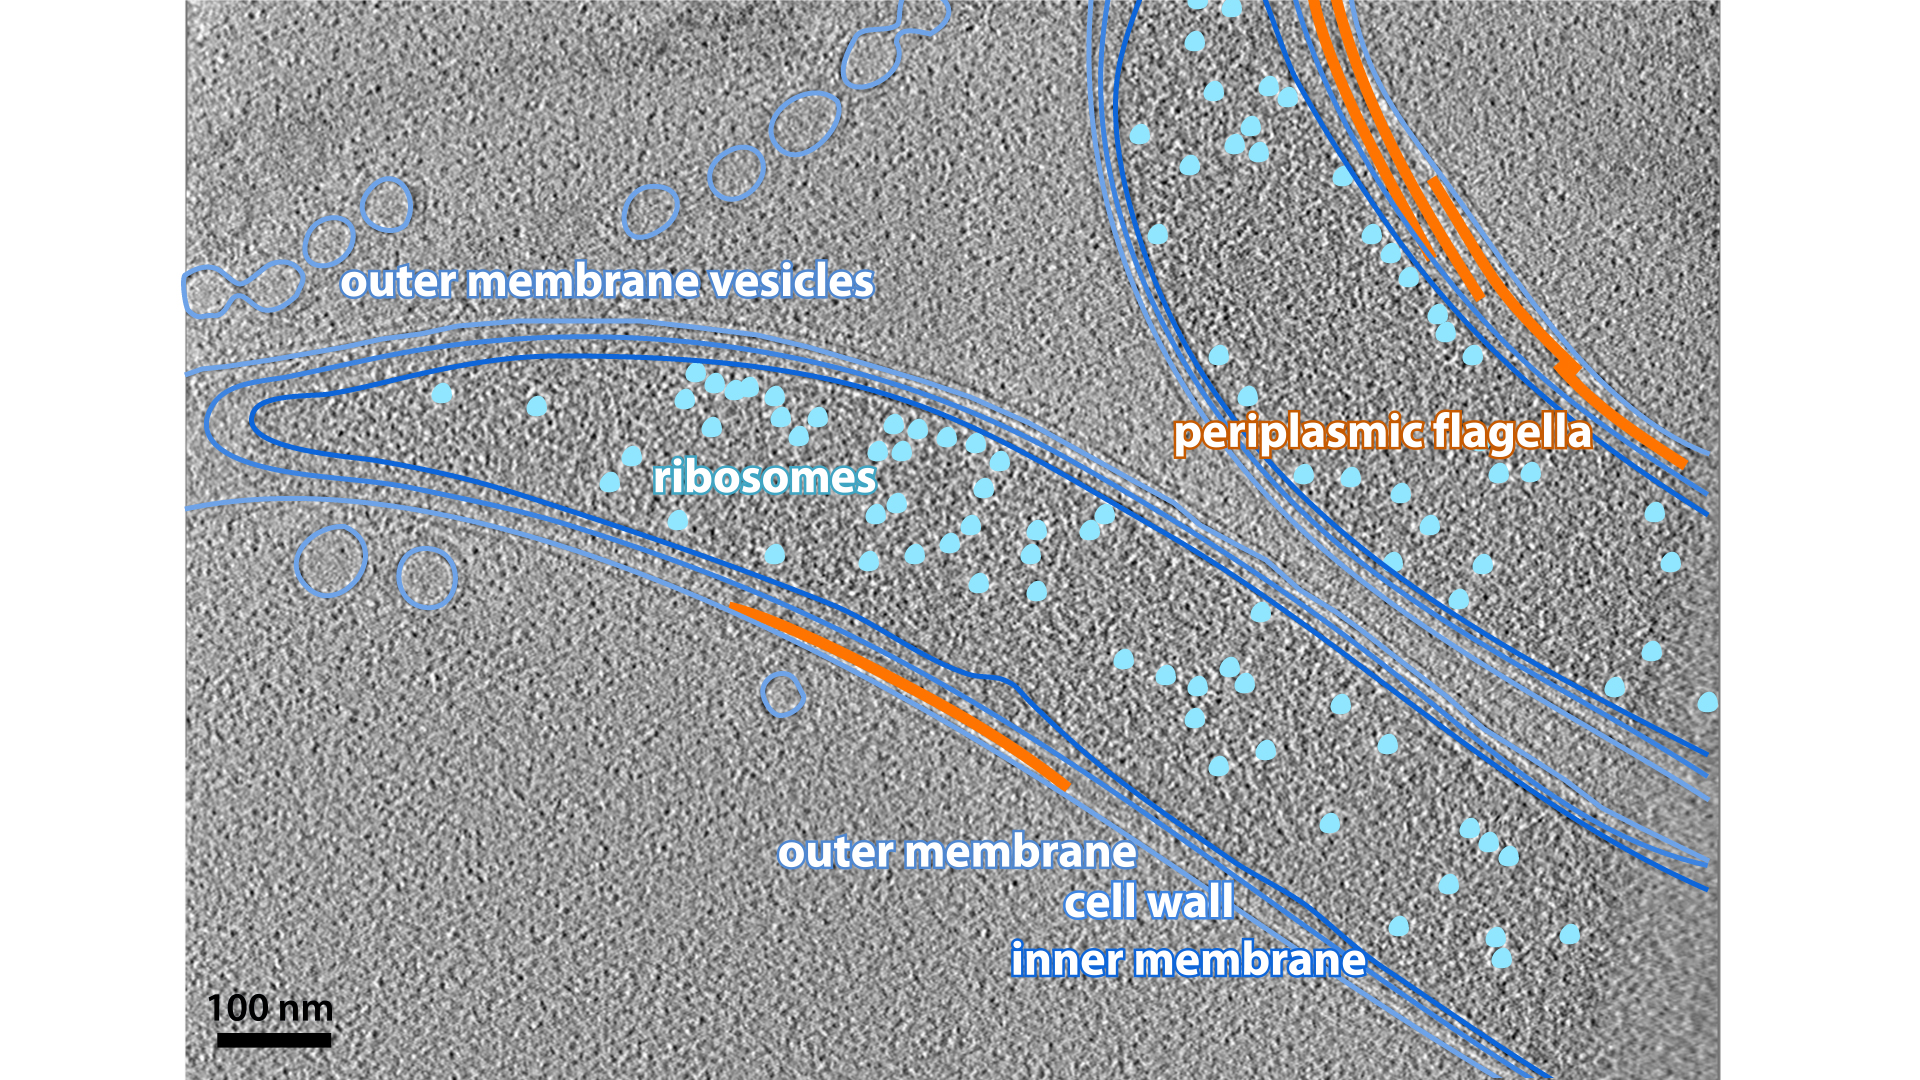
\includegraphics{img/2_4_Bburgdorferi} \caption[Borrelia burgdorferi Collected by]{Borrelia burgdorferi Collected by: Ariane Briegel [10.22002/D1.1353](https://doi.org/10.22002/D1.1353)}\label{fig:unnamed-chunk-11}
\end{figure}

\hypertarget{Vesicle_morphologies}{\subsection{Borrelia
burgdorferi}\label{Vesicle_morphologies}}

Different species can produce outer membrane vesicles that look very
different. The same species can also produce vesicles that look very
different. Sometimes they come off the cell as a chain of spheres;
sometimes the spheres remain connected, like a string of pearls;
sometimes vesicles form long tubes instead, like from this Borrelia
burgdorferi cell. Sometimes the same chain can be tubular in one section
(usually at the base, connected to the cell), and a string of spheres in
another.

\begin{figure}
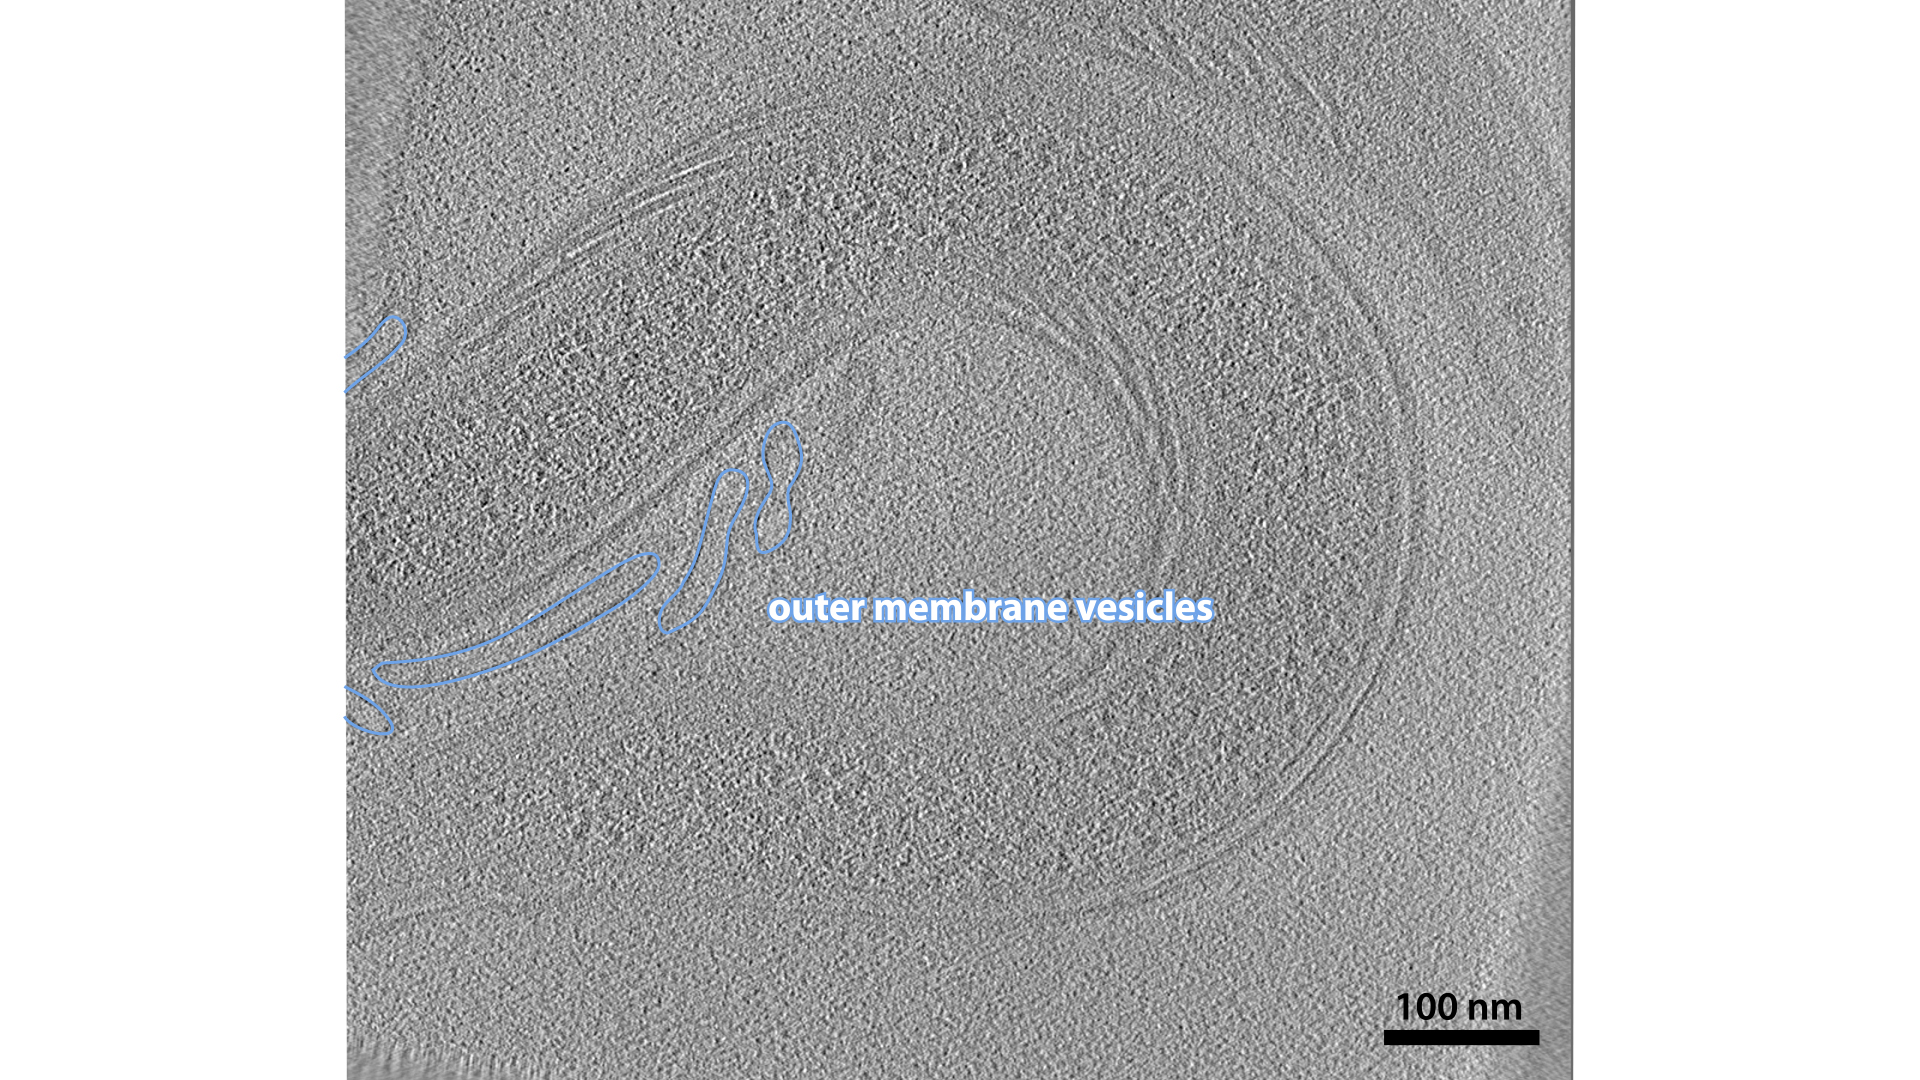
\includegraphics{img/2_4a_Bburgdorferi} \caption[Borrelia burgdorferi 2 Collected by]{Borrelia burgdorferi 2 Collected by: Ariane Briegel [10.22002/D1.1363](https://doi.org/10.22002/D1.1363)}\label{fig:unnamed-chunk-12}
\end{figure}

\subsection{Myxococcus xanthus}\label{Inner_membrane_vesicles}

Not all vesicles come from the outer membrane. The cytoplasmic or inner
membrane can also form vesicles that are released into the cytoplasm, as
in this Myxococcus xanthus cell, or into the periplasm. This seems to be
a less regulated process than outer membrane vesicle formation, and we
see it in many species when they are stressed by low nutrients or high
cell density, suggesting that it is a general phenomenon. Cells shrink
in harsh conditions (more on that in Chapter 7), so cytoplasmic or
periplasmic vesicles may simply offer a place to put the extra membrane
or, more optimistically, to store it until the time comes to grow again.
Just as with outer membrane vesicles, the appearance of cytoplasmic
vesicles can vary widely
\protect\hyperlink{Cytoplasmic_vesicle_variety}{More: Cytoplasmic
vesicle variety}.

\begin{figure}
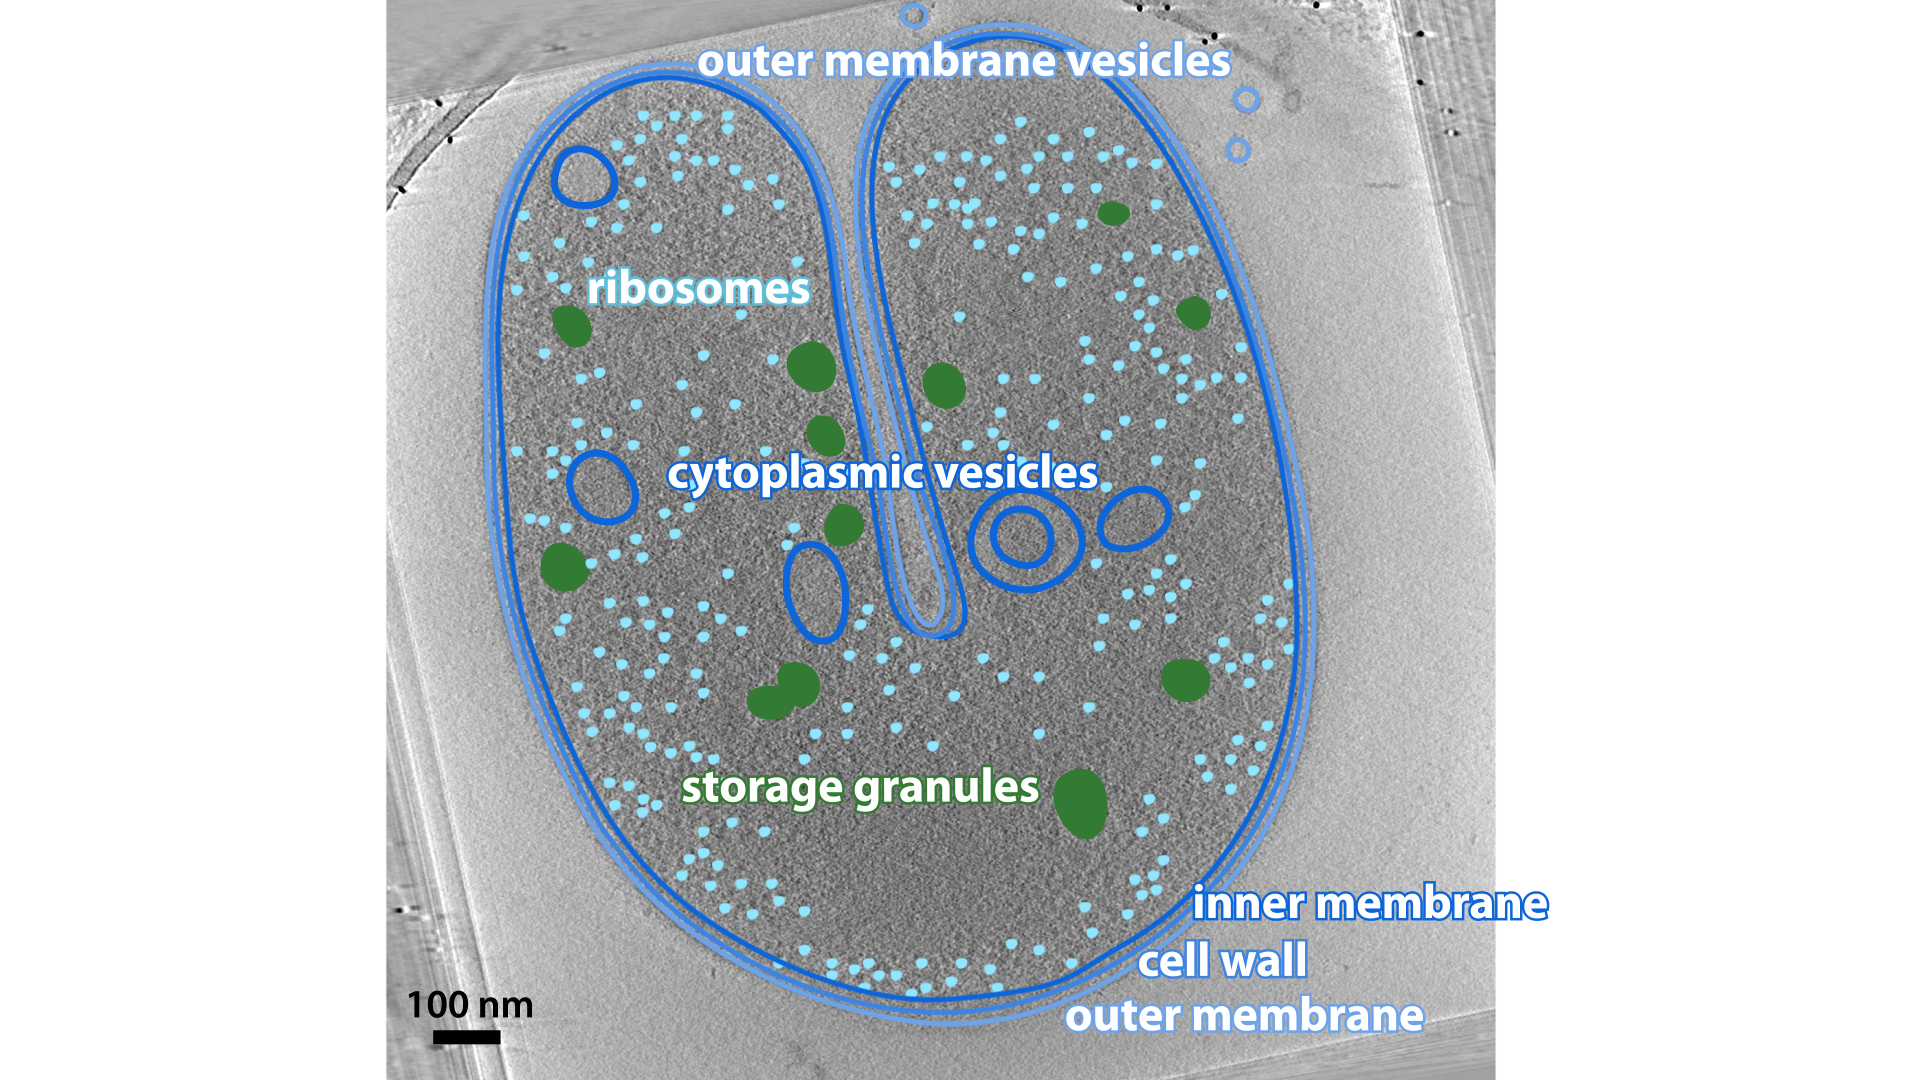
\includegraphics{img/2_4b_Mxanthus} \caption[Myxococcus xanthus Collected by]{Myxococcus xanthus Collected by: Matthew Swulius [10.22002/D1.1364](https://doi.org/10.22002/D1.1364)}\label{fig:unnamed-chunk-13}
\end{figure}

\hypertarget{Cytoplasmic_vesicle_variety}{\subsection{Prosthecobacter
debontii}\label{Cytoplasmic_vesicle_variety}}

Cytoplasmic vesicles exhibit a variety of sizes and shapes. Some are
nested, with vesicles inside vesicles. In this Prosthecobacter debontii
cell, you can see two other morphologies. One is a large, flattened
horseshoe-shaped vesicle. Another is a more typical spherical shape, but
is decorated with what looks like protein complexes.

This cell also has unusual structures on its surface that have yet to be
identified.

\begin{figure}
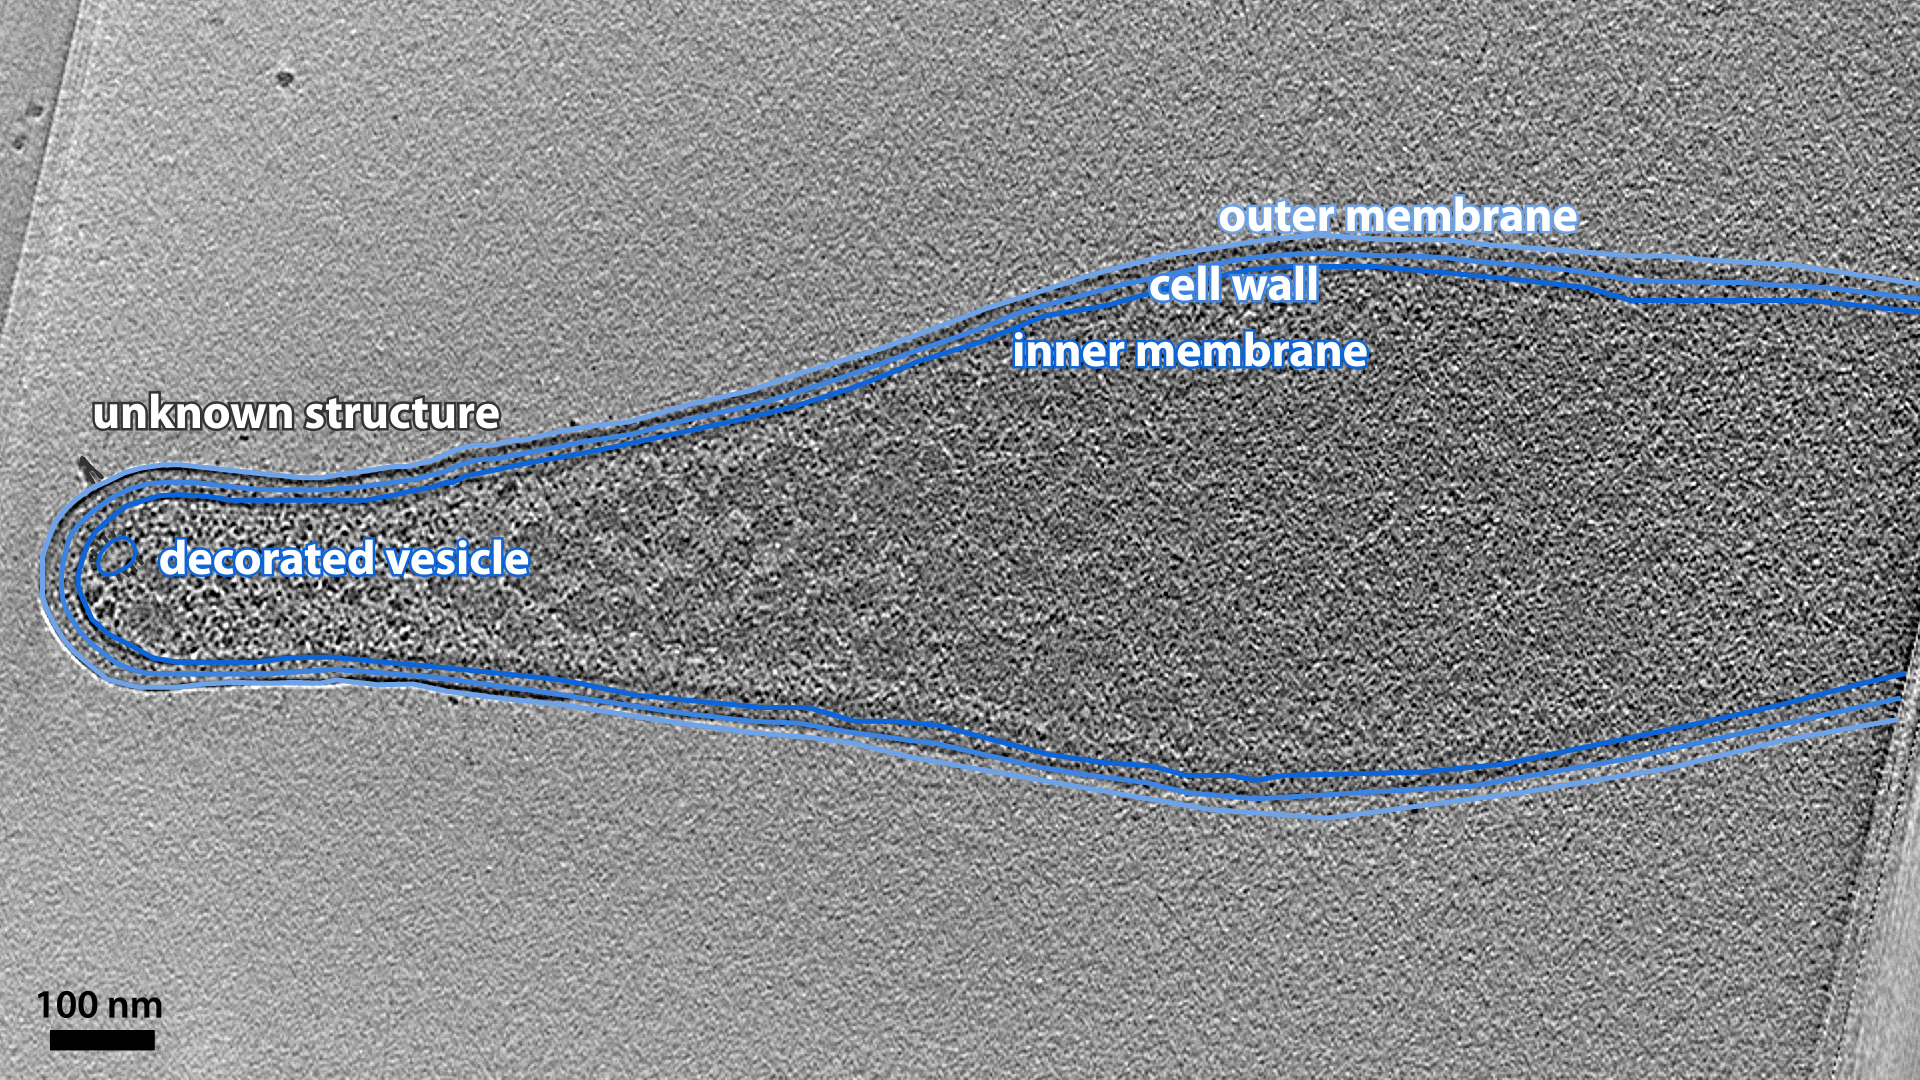
\includegraphics{img/2_4c_Pdebontii} \caption[Prosthecobacter debontii Collected by]{Prosthecobacter debontii Collected by: Martin Pilhofer [10.22002/D1.1365](https://doi.org/10.22002/D1.1365)}\label{fig:unnamed-chunk-14}
\end{figure}

\section{Mycoplasma marinum}\label{mycoplasma-marinum}

Evolution is endlessly creative, providing exceptions to nearly every
classification rule. We've just described a neat breakdown of bacteria
into monoderms (one membrane, thick sacculus, positive Gram stain) and
diderms (two membranes, thin sacculus, negative Gram stain). But some
cells, like this Mycobacterium marinum, defy classification.
Mycobacteria are diderm, with an inner and an outer membrane, and a cell
wall. But they have unique molecules (named mycolic acids in their
honor) in the outer membrane. These acids interfere with Gram staining,
yielding an intermediate result between positive and negative. And their
sacculus consists of three layers, each with a unique molecular
composition \protect\hyperlink{Mycobacterial_architecture}{Schematic --
Mycobacterial architecture}. In this case, the middle layer is the
familiar peptidoglycan.

When you look at the schematic, you'll see another layer outside the
outer membrane. This layer, the capsule, isn't visible in the movie of
the cell, though. It is made up of ``Extracellular Polymeric
Substance,'' abbreviated EPS, or long chains of sugars, sometimes linked
to the outer membrane and sometimes free-floating. These sugars don't
interact strongly with electrons, so the capsule is usually invisible by
electron microscopy. But in fact, many bacteria (mostly diderm, but also
some monoderm) have a capsule. The capsule can help bacteria attach onto
surfaces and offers an extra layer of protection, trapping water to
prevent desiccation and making it more difficult for hydrophobic
molecules like detergents to get through to disrupt the membranes. It
also makes it more difficult for viruses to reach the cell, and for
eukaryotic ``predators'' like macrophages to eat it.

\begin{figure}
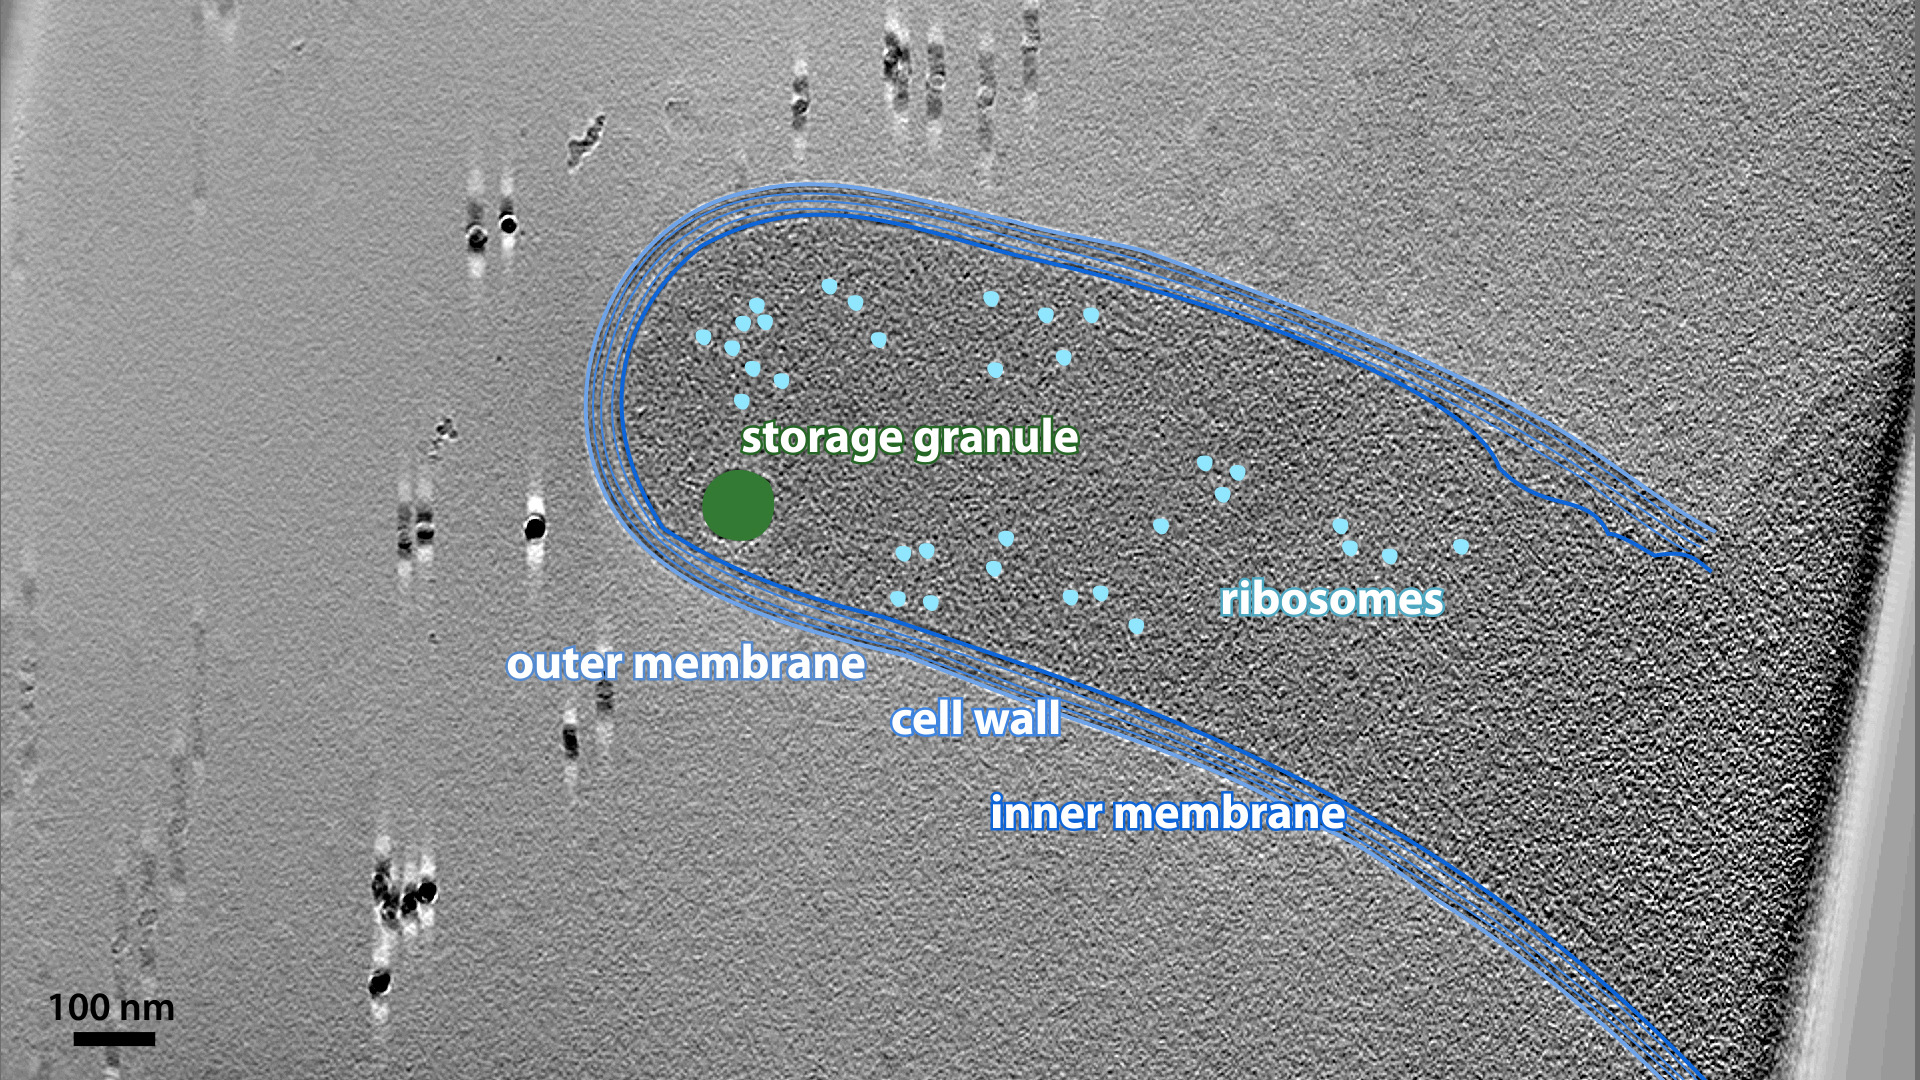
\includegraphics{img/2_5_Mmarinum} \caption[Mycobacterium marinum Collected by]{Mycobacterium marinum Collected by: Elitza Tocheva [10.22002/D1.1354](https://doi.org/10.22002/D1.1354)}\label{fig:unnamed-chunk-15}
\end{figure}

\hypertarget{Mycobacterial_architecture}{\subsection{Mycobacterial
architecture}\label{Mycobacterial_architecture}}

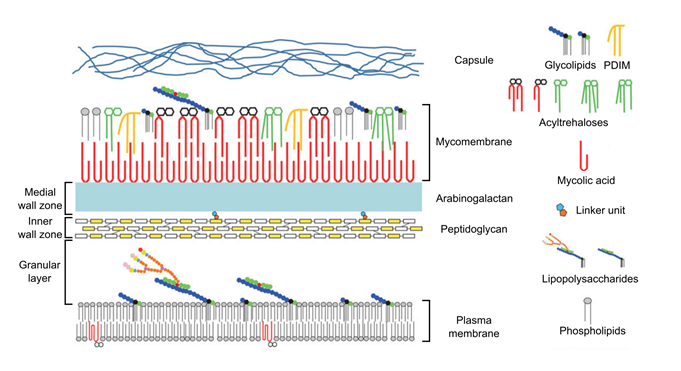
\includegraphics{img/02_schematic/2_5_1_Mycobacteria}

A unique architecture encloses Mycobacterial cells. Note the outer
membrane, with lipids only in the outer leaflet, and mycolic acids
forming the inner. Note also the multiple strata of sugars in the cell
wall. Also note the capsule depicted outside the outer membrane.

\section{Caulobacter crescentus}\label{caulobacter-crescentus}

How else can you protect your cell from the rigors of a harsh world?
What about encasing it in an armored shell a la the armadillo? Many
bacteria (both monoderms and diderms) and archaea use modular proteins
for this purpose, interlocking Lego-block-like pieces into a shell
called the Surface Layer, or S-layer. You can guess that this must offer
a significant evolutionary advantage since up to 15\% of the total
protein in the cell can be found in the structure. In fact, S-layers
play many roles for cells, some of which you'll see on the next page,
but one of their main functions is as a gatekeeper, preventing large
things like viruses from reaching the membrane.

S-layers are crystalline lattices, and they can be striking in
appearance, as on this Caulobacter crescentus cell. Amazingly, the
lattice is made from (many copies of) a single protein
\protect\hyperlink{S-layer_architecture}{Schematic -- S-layer
architecture}. The pinwheel-like subunits interact laterally, leaving
pores large enough for nutrients to pass through, but not large enough
for viruses. The modular nature of the lattice means that units can be
popped in as the cell grows, or popped out to allow a cell appendage to
poke through. In general, S-layers are quite accommodating; they don't
even interfere with the production of outer membrane vesicles
\protect\hyperlink{Nanopods}{More: Nanopods}. S-layer proteins can also
be modified to alter their properties; for instance attachment of a
sugar can enable them to stick the cell to a surface.

\begin{figure}
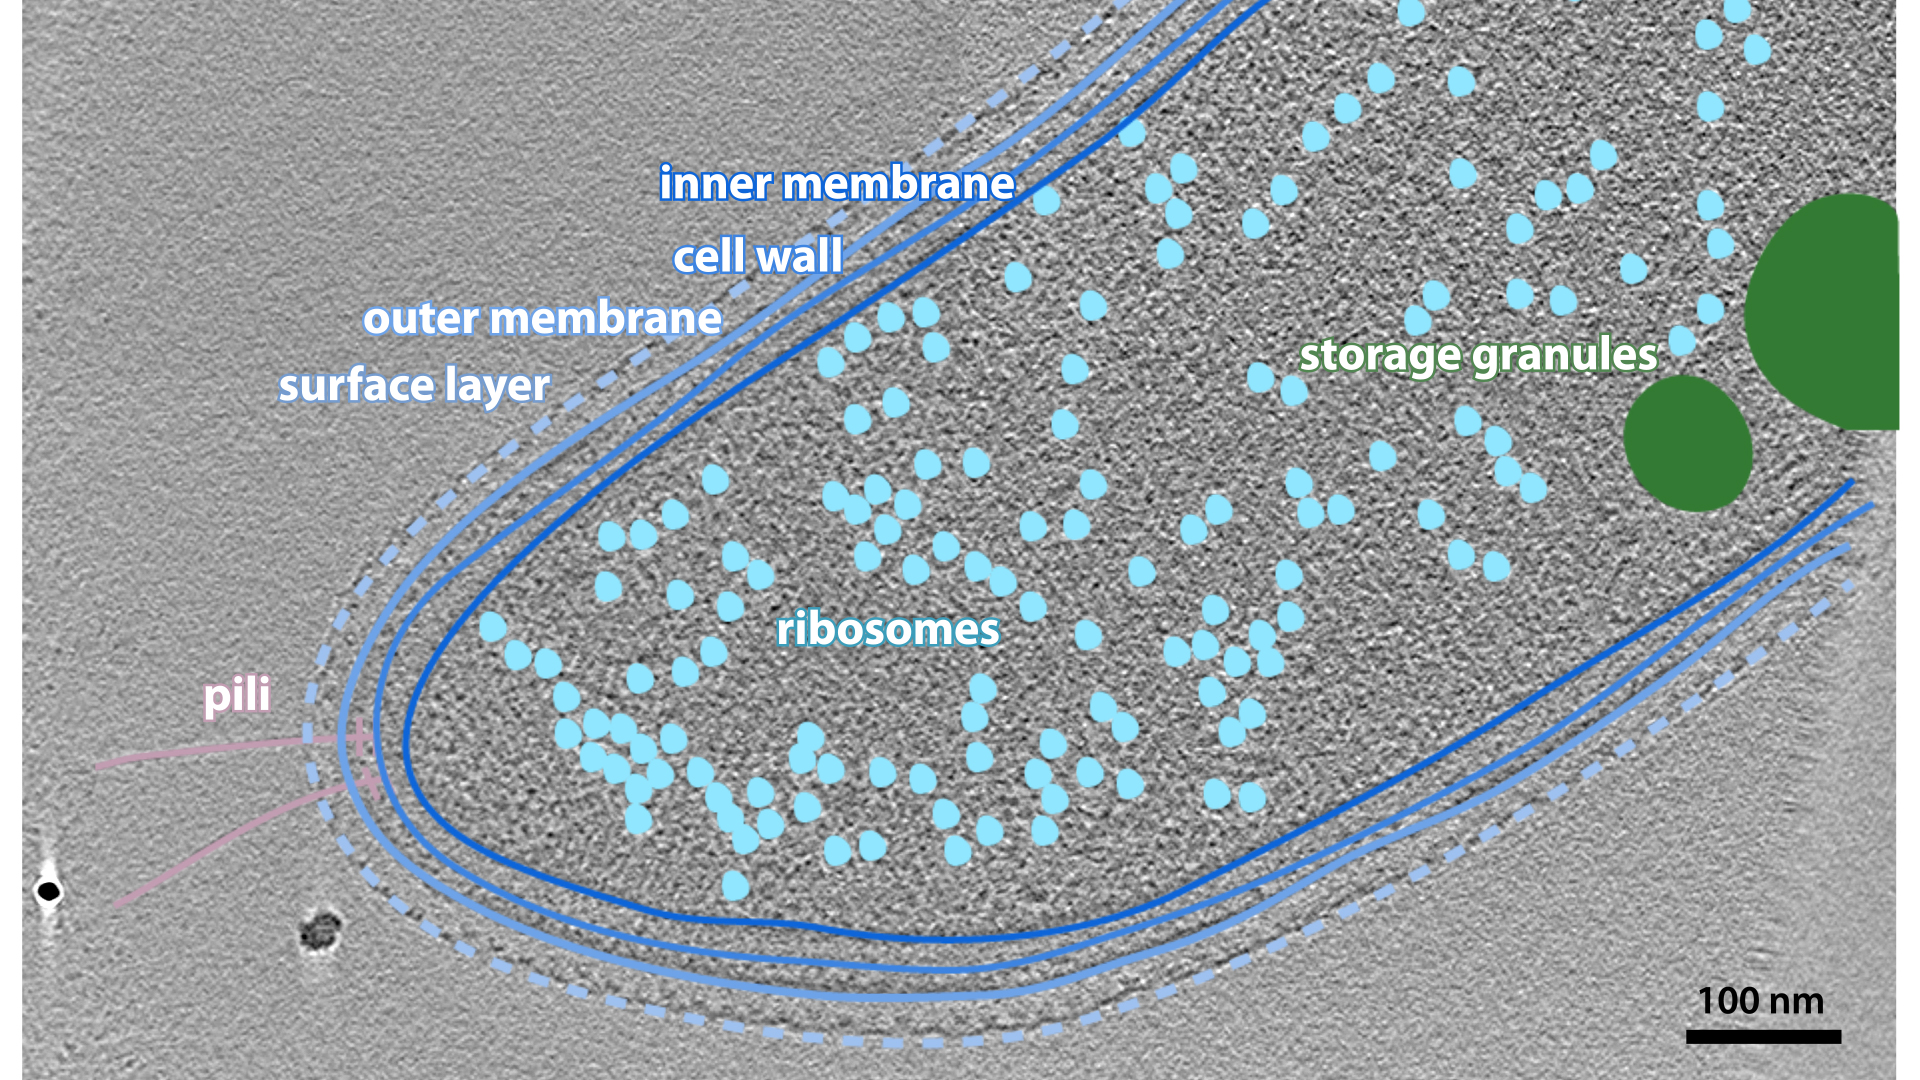
\includegraphics{img/2_6_Ccrescentus} \caption[Caulobacter crescentus Collected by]{Caulobacter crescentus Collected by: Ariane Briegel [10.22002/D1.1355](https://doi.org/10.22002/D1.1355)}\label{fig:unnamed-chunk-17}
\end{figure}

\hypertarget{S-layer_architecture}{\subsection{S-layer
architecture}\label{S-layer_architecture}}

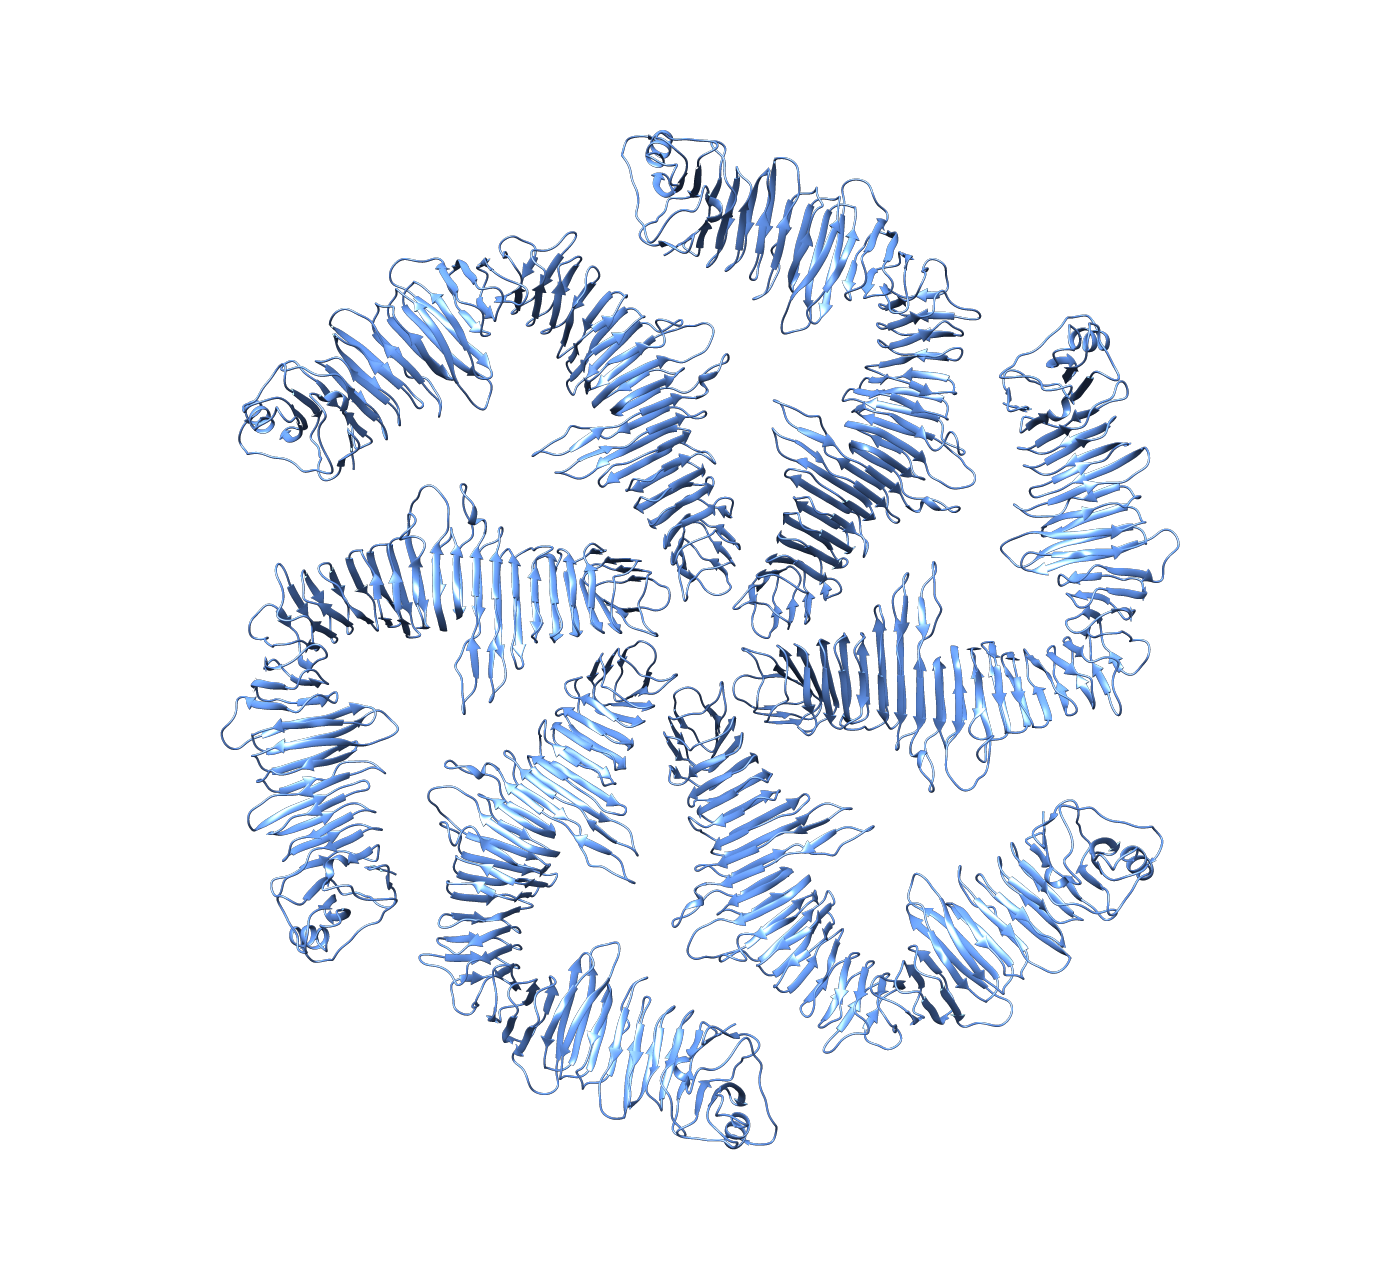
\includegraphics{img/02_schematic/2_6_1_SLayerTop}

A single protein forms the S-layer you just saw in Caulobacter
crescentus. The protein has two domains. The bottom domain anchors to
lipoproteins attached to the outer membrane. The top domain forms the
canopy of the S-layer, organizing hierarchically into hexameric rosettes
like this that in turn pack into a larger hexameric lattice. This
lattice is flexible enough to curve around even narrow regions of the
cell (more on this stalk in Chapter 3).

\hypertarget{Nanopods}{\subsection{Delftia acidovorans}\label{Nanopods}}

Archaea and diderm bacteria with S-layers produce characteristic outer
membrane vesicles: they bud off with the S-layer attached. Delftia
acidovorans, like this produce so-called nanopods: chains of outer
membrane vesicles ensheathed in S-layer.

\begin{figure}
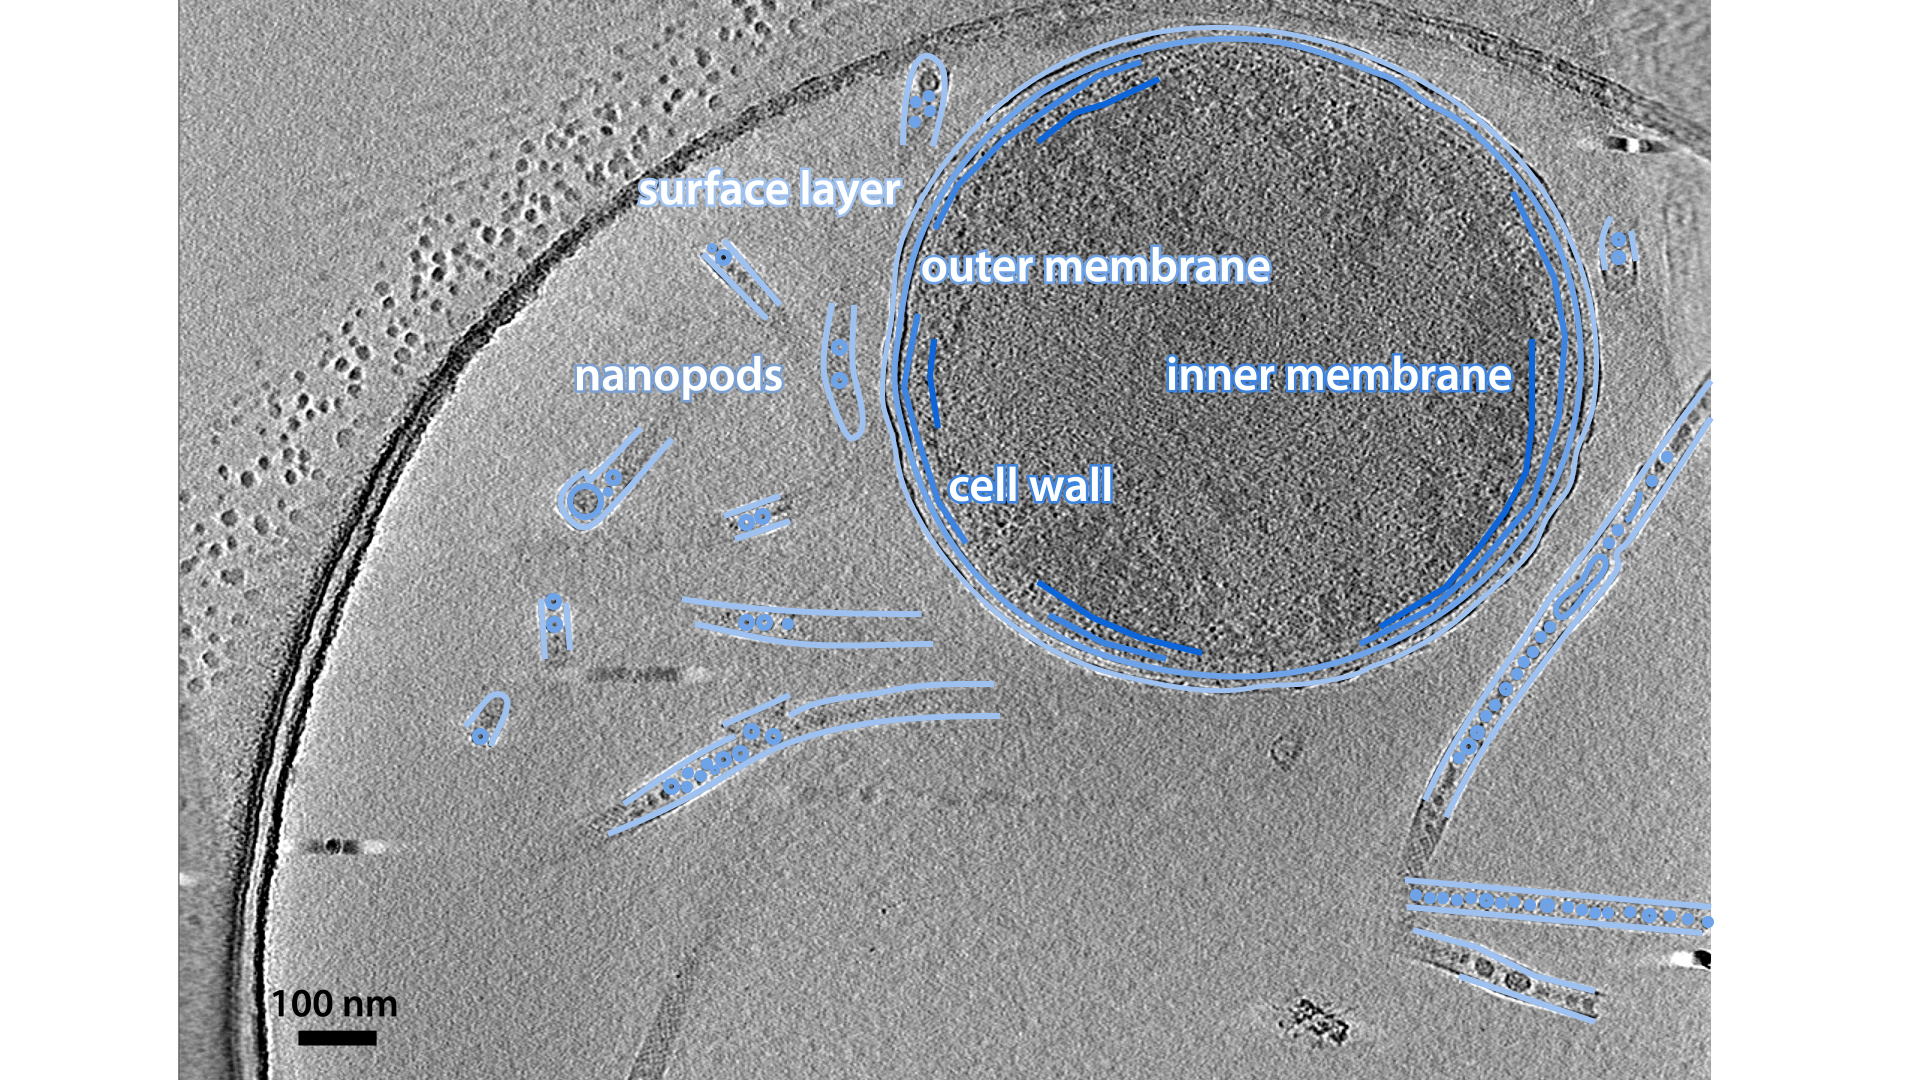
\includegraphics{img/2_6a_Dacidovorans} \caption[Delftia acidovorans Collected by]{Delftia acidovorans Collected by: Elitza Tocheva [10.22002/D1.1366](https://doi.org/10.22002/D1.1366)}\label{fig:unnamed-chunk-19}
\end{figure}

\section{Sulfolobus solfataricus}\label{sulfolobus-solfataricus}

One of the most striking features of the S-layer is how different it can
look in different species. For instance, compare this archaeal
Sulfolobus solfataricus cell to the bacterium on the last page, or to
other diderm \protect\hyperlink{M._alcaliphilum}{More: M. alcaliphilum}
or monoderm \protect\hyperlink{}{More: C. thermocellum} bacteria, or
archaea \protect\hyperlink{N._maritimus}{More: N. maritimus}
\protect\hyperlink{Methanoregula_formicica}{More: Methanoregula
formicica}. All S-layers are crystalline lattices of a single--or in a
few cases, two--proteins, but the particular pattern of the lattice
depends on the shape of this building block and how it multimerizes into
a higher-order structure. The shape of the building block varies
considerably; there is almost no sequence homology between S-layer
proteins from different species. And shapes come together in different
ways, forming repeating units of one, two, three (as on this cell),
four, or six blocks.

S-layers are very common in archaea like this cell. Most archaea don't
have cell walls, but the S-layer provides the same function of external
scaffolding. Remember, too, that nearly all archaea are monoderms,
lacking the extra periplasmic compartment that diderms have. Here again
the S-layer serves a similar function, enclosing a space around the
cell's membrane called the pseudo-periplasmic space. Just as with the
bacterial periplasm, this space serves as an antechamber for the cell,
restricting access by large molecules. In some cases, the
pseudo-periplasmic space also contains specific proteins that function
in metabolism.

\begin{figure}
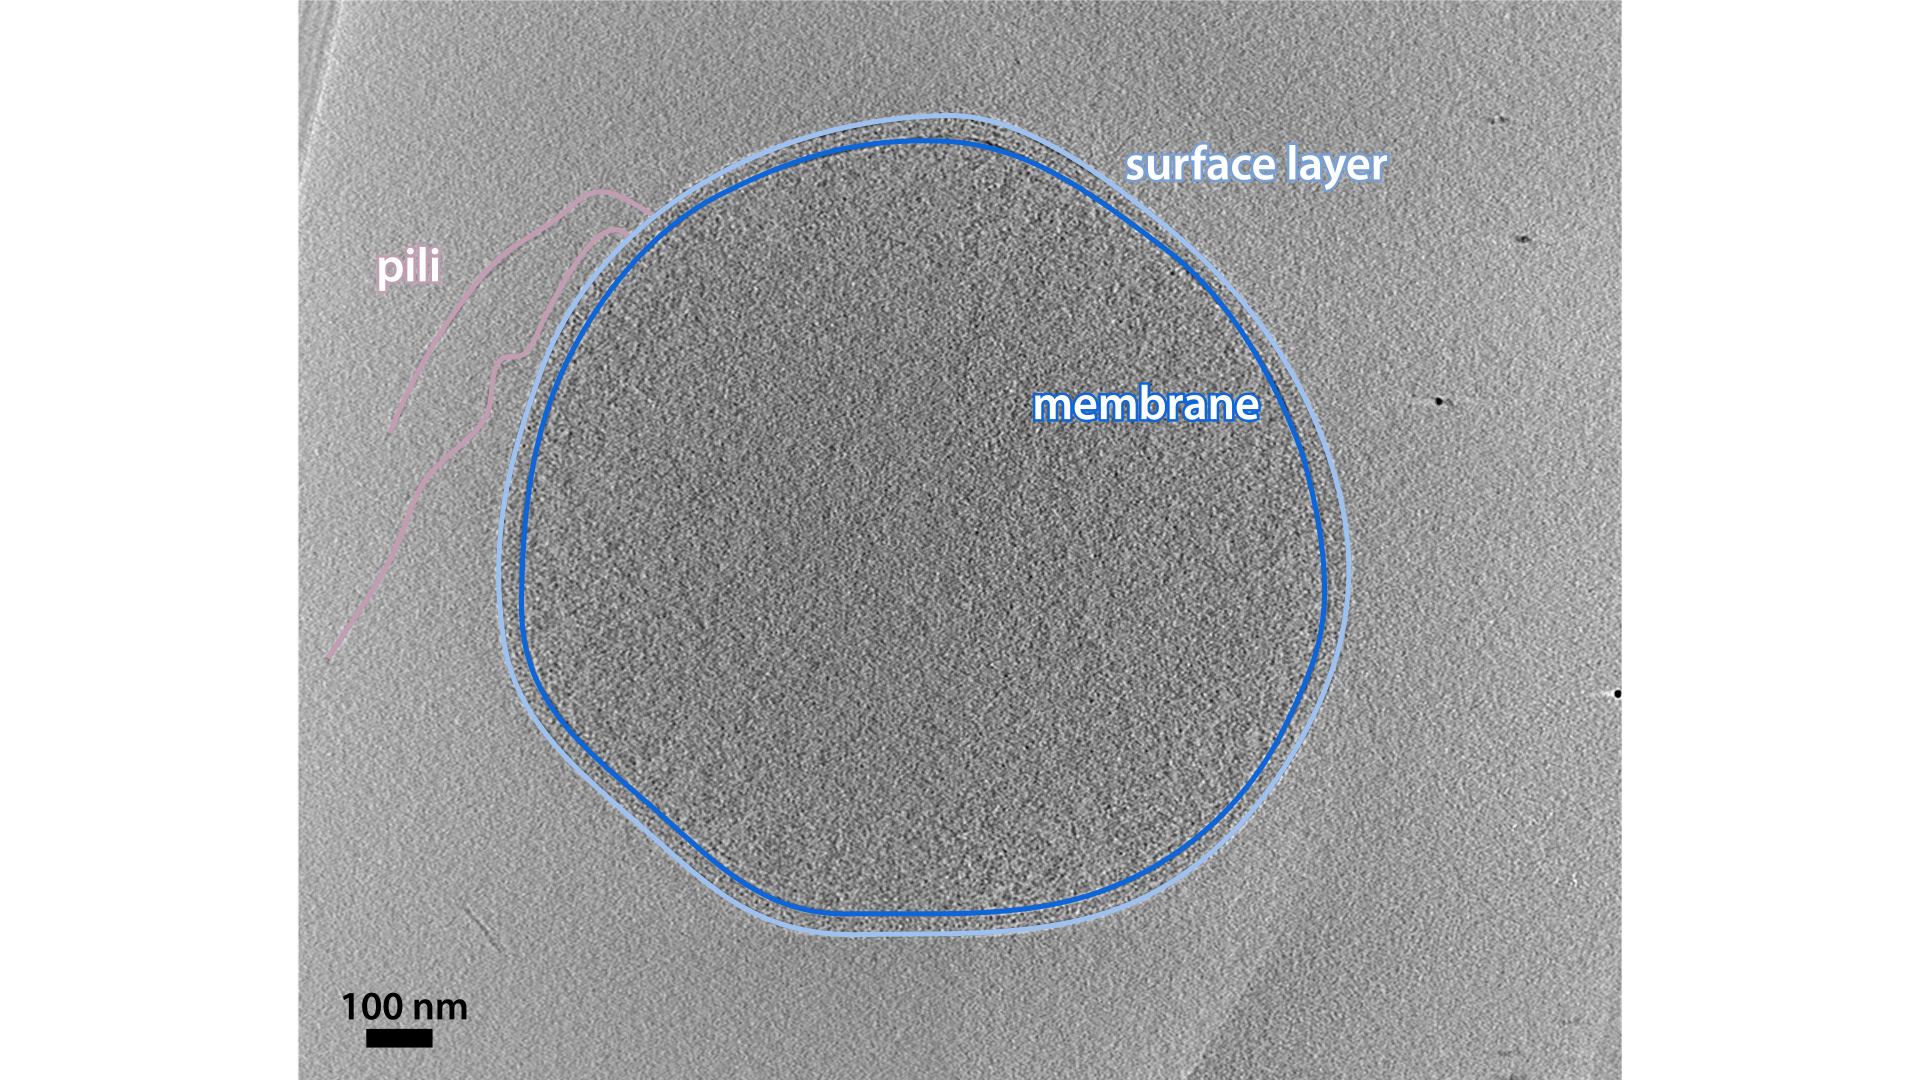
\includegraphics{img/2_7_Ssolfataricus} \caption[Sulfolobus solfataricus Collected by]{Sulfolobus solfataricus Collected by: Lu Gan [10.22002/D1.1356](https://doi.org/10.22002/D1.1356)}\label{fig:unnamed-chunk-20}
\end{figure}

\hypertarget{M._alcaliphilum}{\subsection{Methylomicrobium
alcaliphilum}\label{M._alcaliphilum}}

In Methylomicrobium alcaliphilum, V-shaped S-layer proteins come
together to form cups that pack into a hexagonal pattern.

\begin{figure}
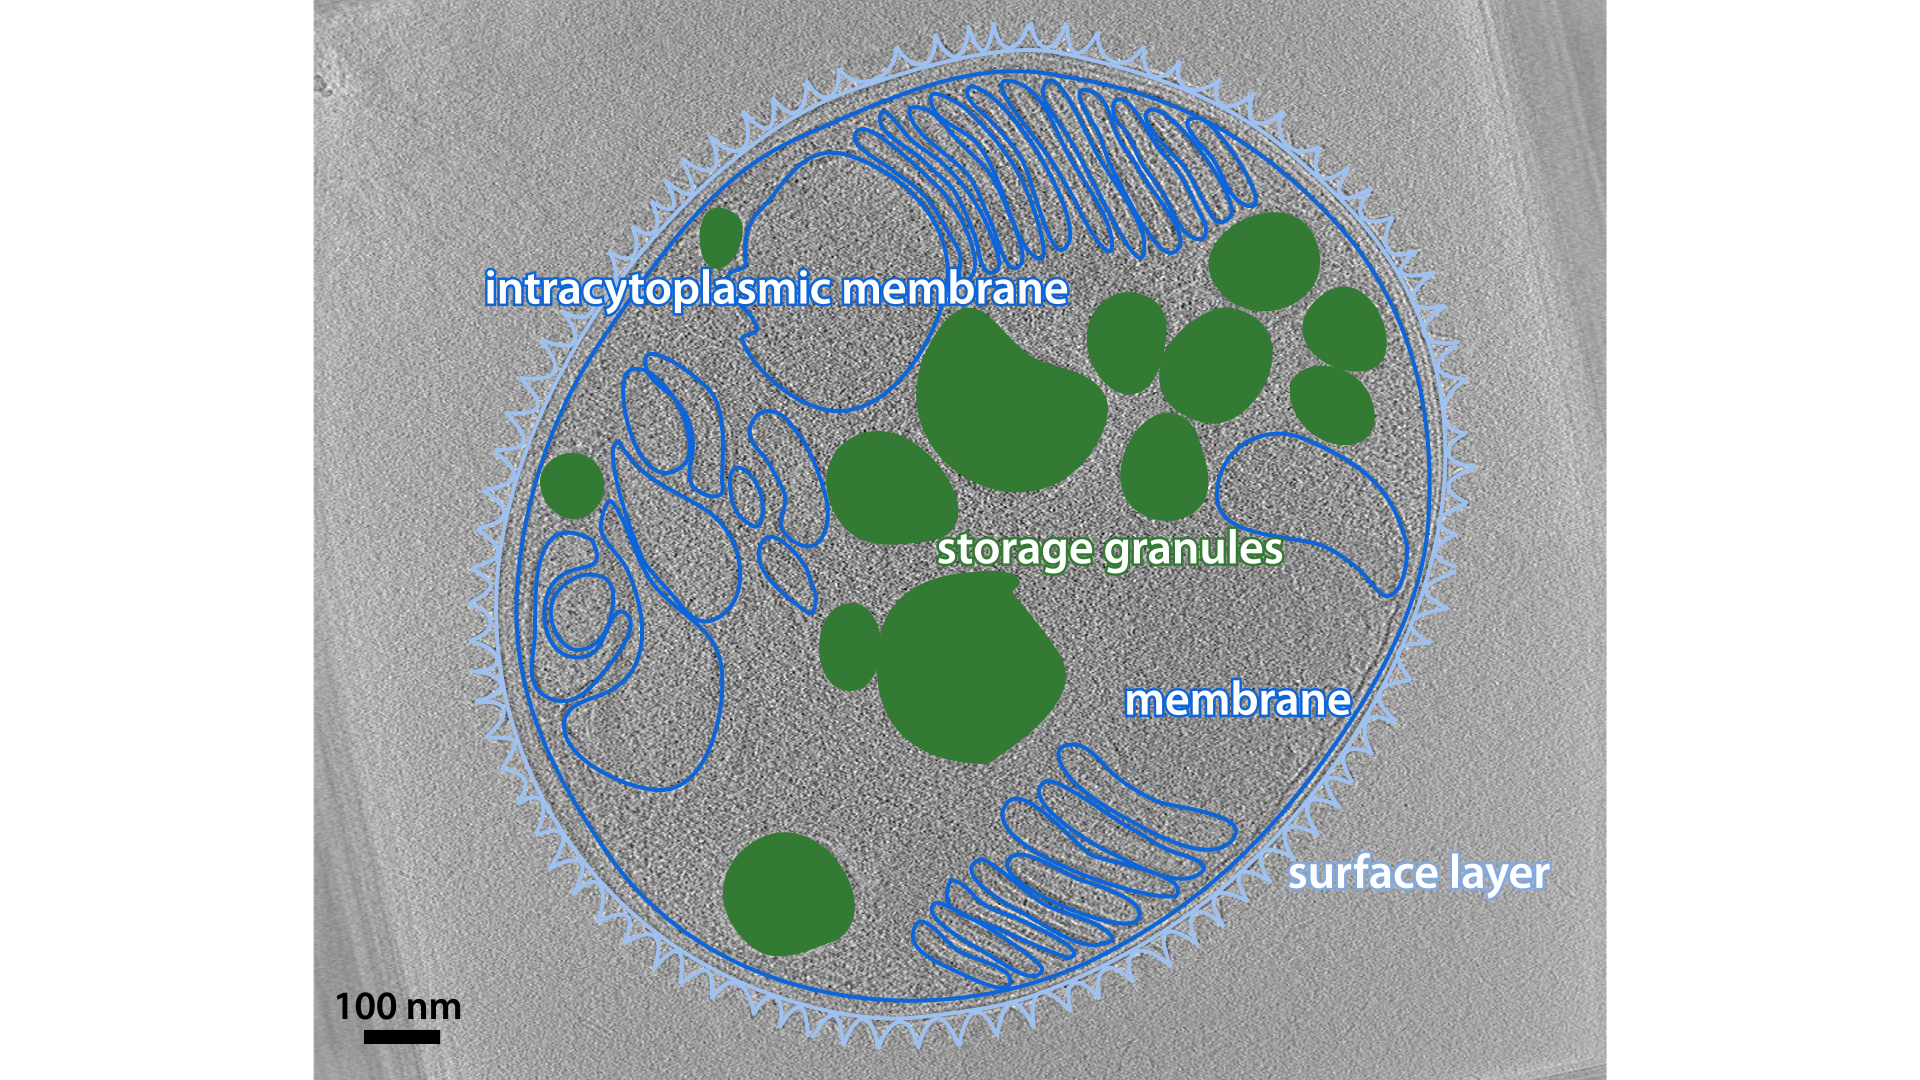
\includegraphics{img/2_7a_Malcaliphilum} \caption[Methylomicrobium alcaliphilum Collected by]{Methylomicrobium alcaliphilum Collected by: Songye Chen [10.22002/D1.1367](https://doi.org/10.22002/D1.1367)}\label{fig:unnamed-chunk-21}
\end{figure}

\hypertarget{N._maritimus}{\subsection{Nitrosopumilis
maritimus}\label{N._maritimus}}

In Nitrosopumilis maritimus, S-layer proteins form hexagonal rosettes
that in turn pack into a hexagonal lattice.

\begin{figure}
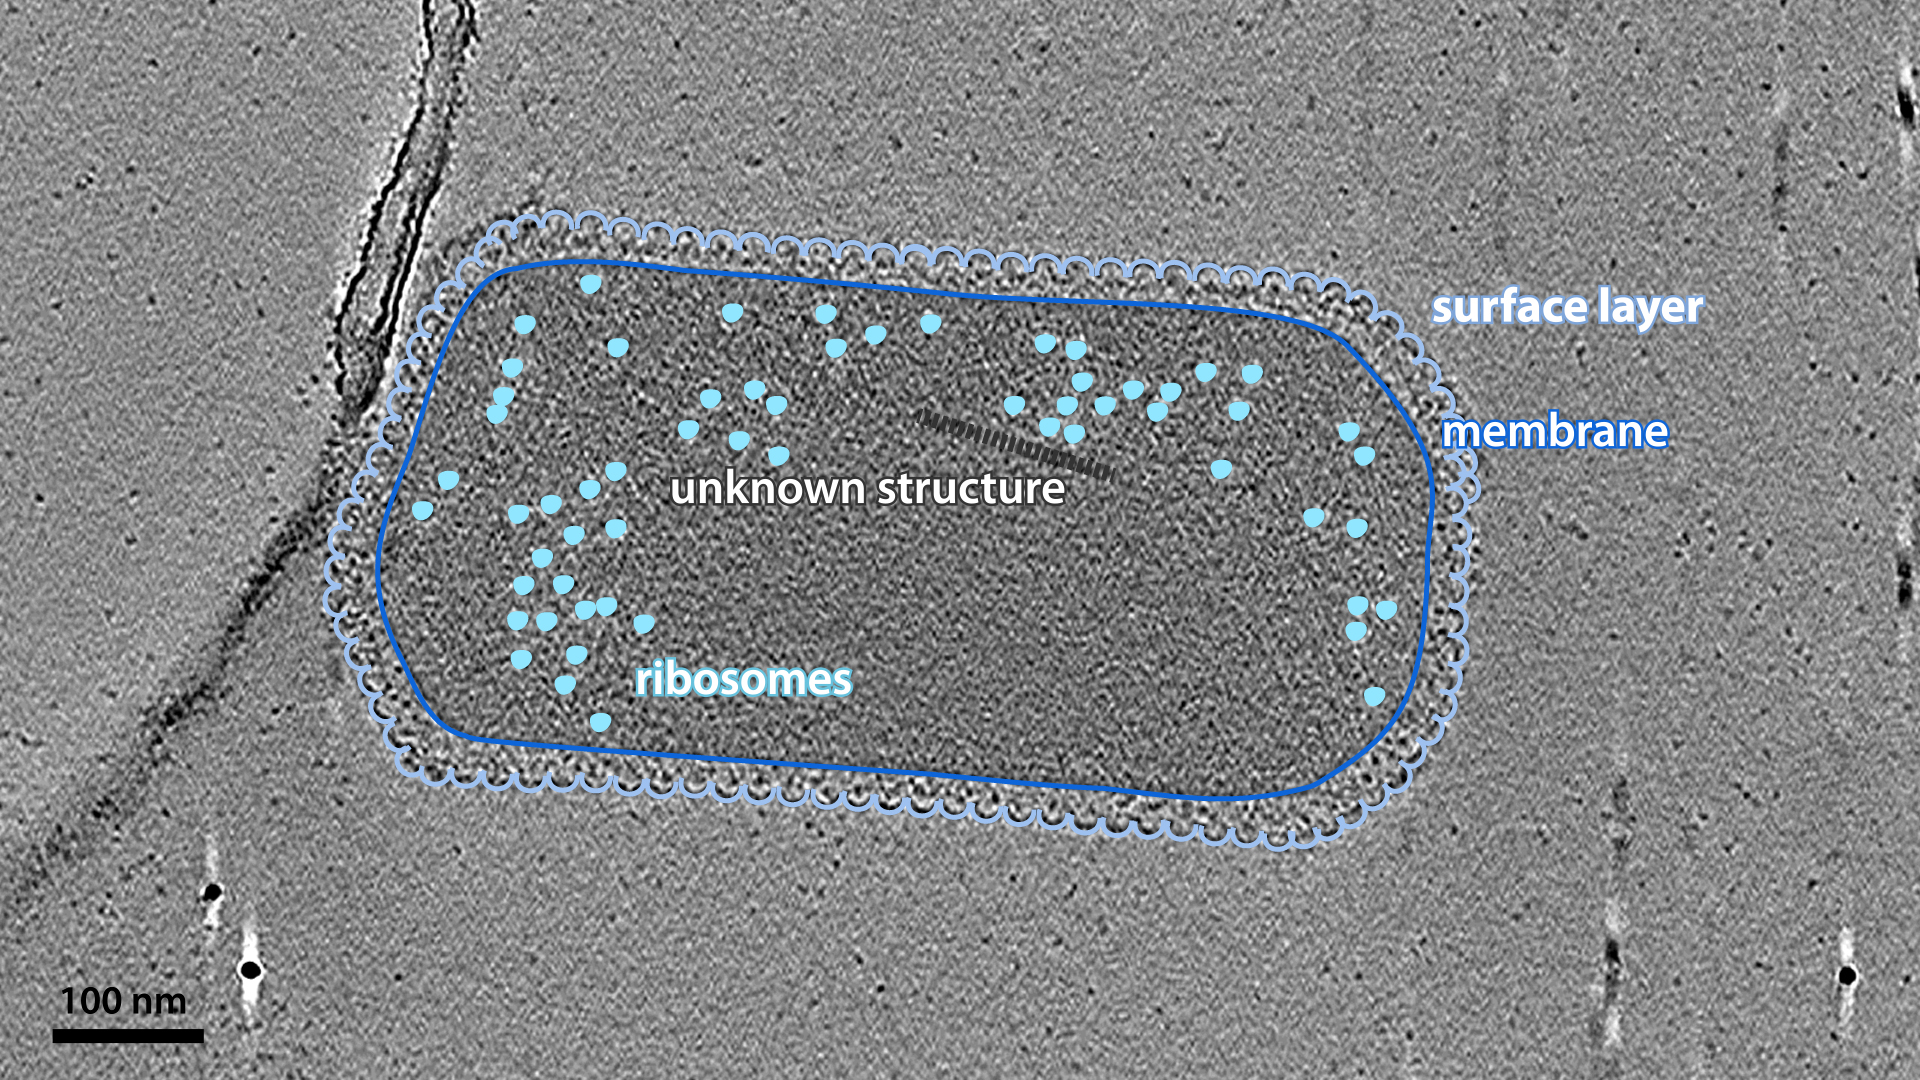
\includegraphics{img/2_7c_Nmaritimus} \caption[Nitrosopumilis maritimus Collected by]{Nitrosopumilis maritimus Collected by: Rasika Ramdasi [10.22002/D1.1368](https://doi.org/10.22002/D1.1368)}\label{fig:unnamed-chunk-22}
\end{figure}

\hypertarget{Methanoregula_formicica}{\subsection{Methanoregula
formicica}\label{Methanoregula_formicica}}

\begin{figure}
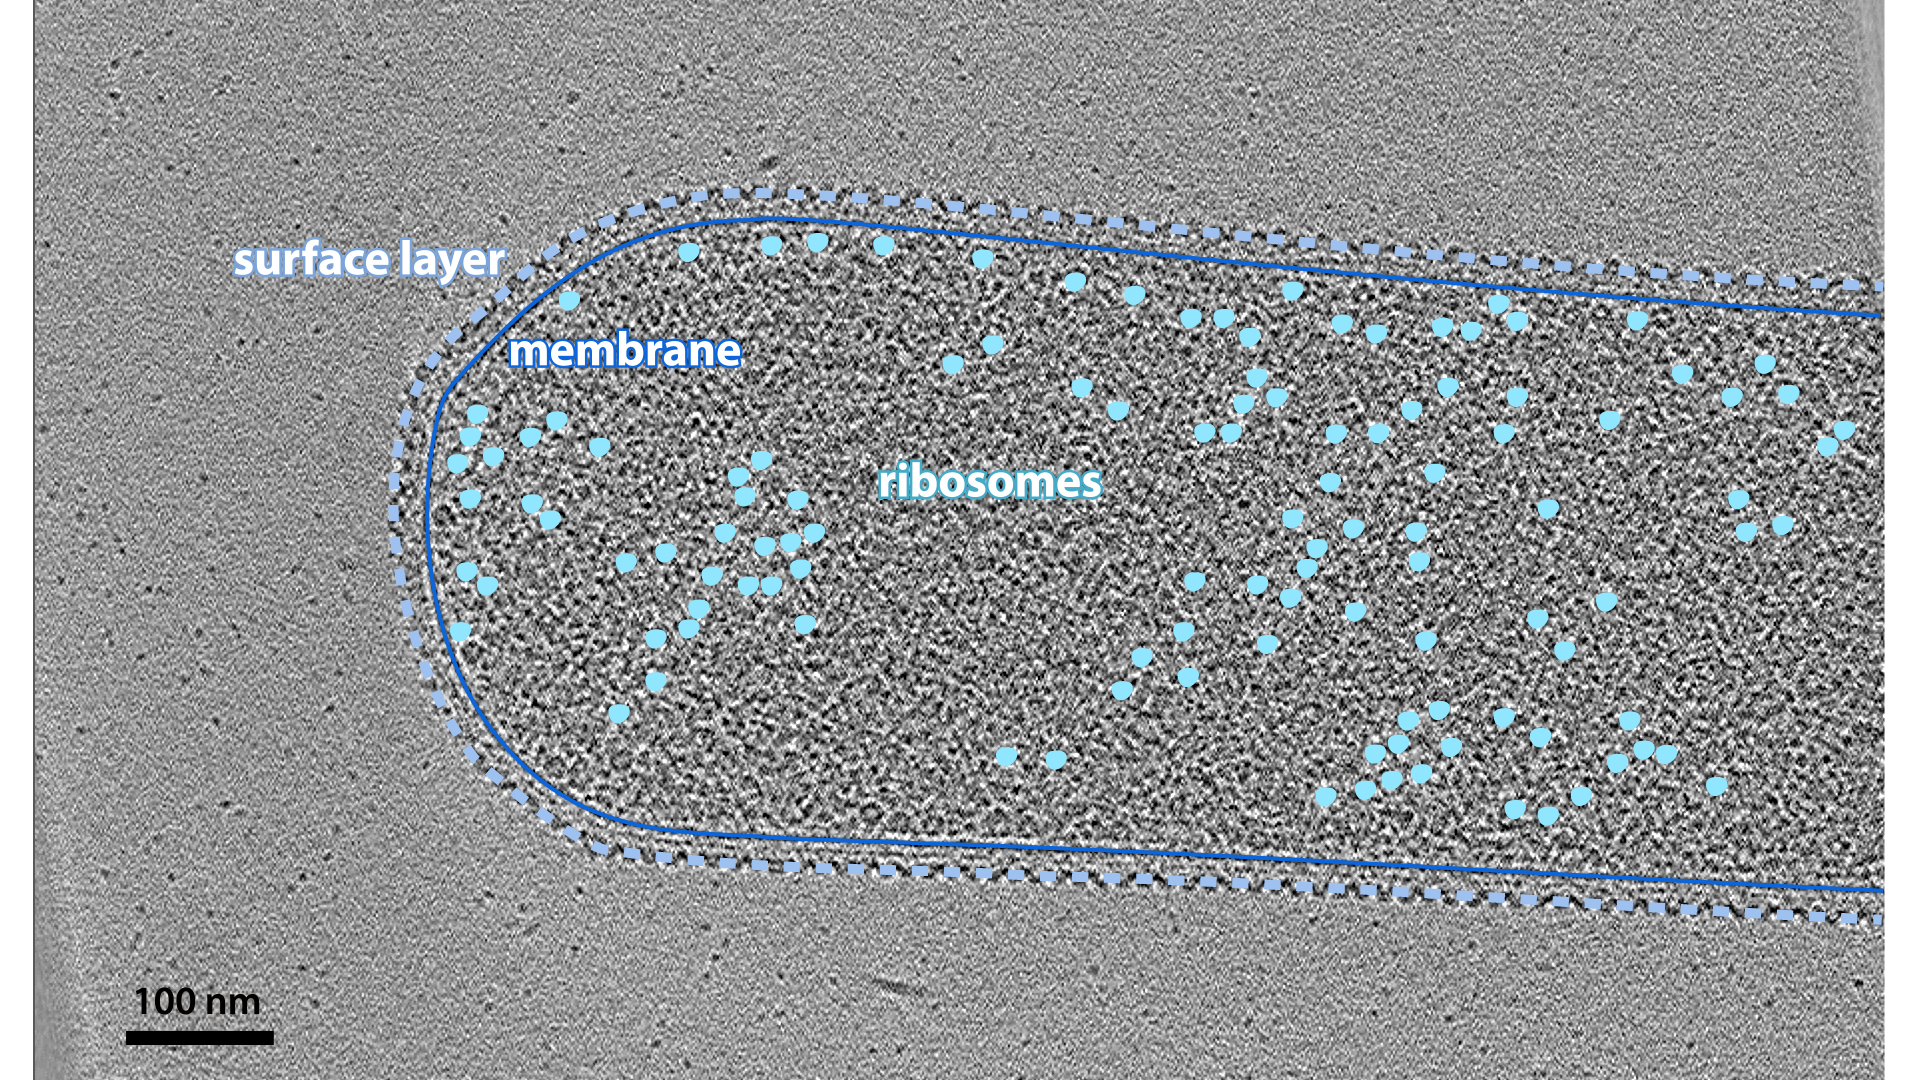
\includegraphics{img/2_7d_Mformicica} \caption[Methanoregula formicica Collected by]{Methanoregula formicica Collected by: Ariane Briegel [10.22002/D1.1369](https://doi.org/10.22002/D1.1369)}\label{fig:unnamed-chunk-23}
\end{figure}

\section{Methanospirillum hungatei}\label{methanospirillum-hungatei}

Why stop with a single layer of protein? For proof that Nature is
endlessly inventive, consider this Methanospirillum hungatei cell. These
archaea encase themselves in an S-layer, and then an additional protein
layer that forms a highly impermeable sheath. The sheath is also very
resistant to pressure, which could be important in the cells' line of
work. M. hungatei were discovered in sewage, where they break down
organic waste, producing methane. One theory is that the sheath acts as
a pressure regulator; when enough methane builds up inside the cell, the
pressure expands the sheath, opening its pores wide enough to allow the
methane to dissipate and new metabolic substrates like hydrogen and
carbon dioxide to enter.

The rules of architecture remain the same, though. Just as in the
bacterial cell wall, sheath polymers are arranged as hoops perpendicular
to the long axis of the rod-shaped cell. The ends of the sheath, as you
can see, are special, with multiple protein layers stacking into a thick
plug. Cells divide within the sheath, and long chains of cells in a
continuous sheath are often observed.

\begin{figure}
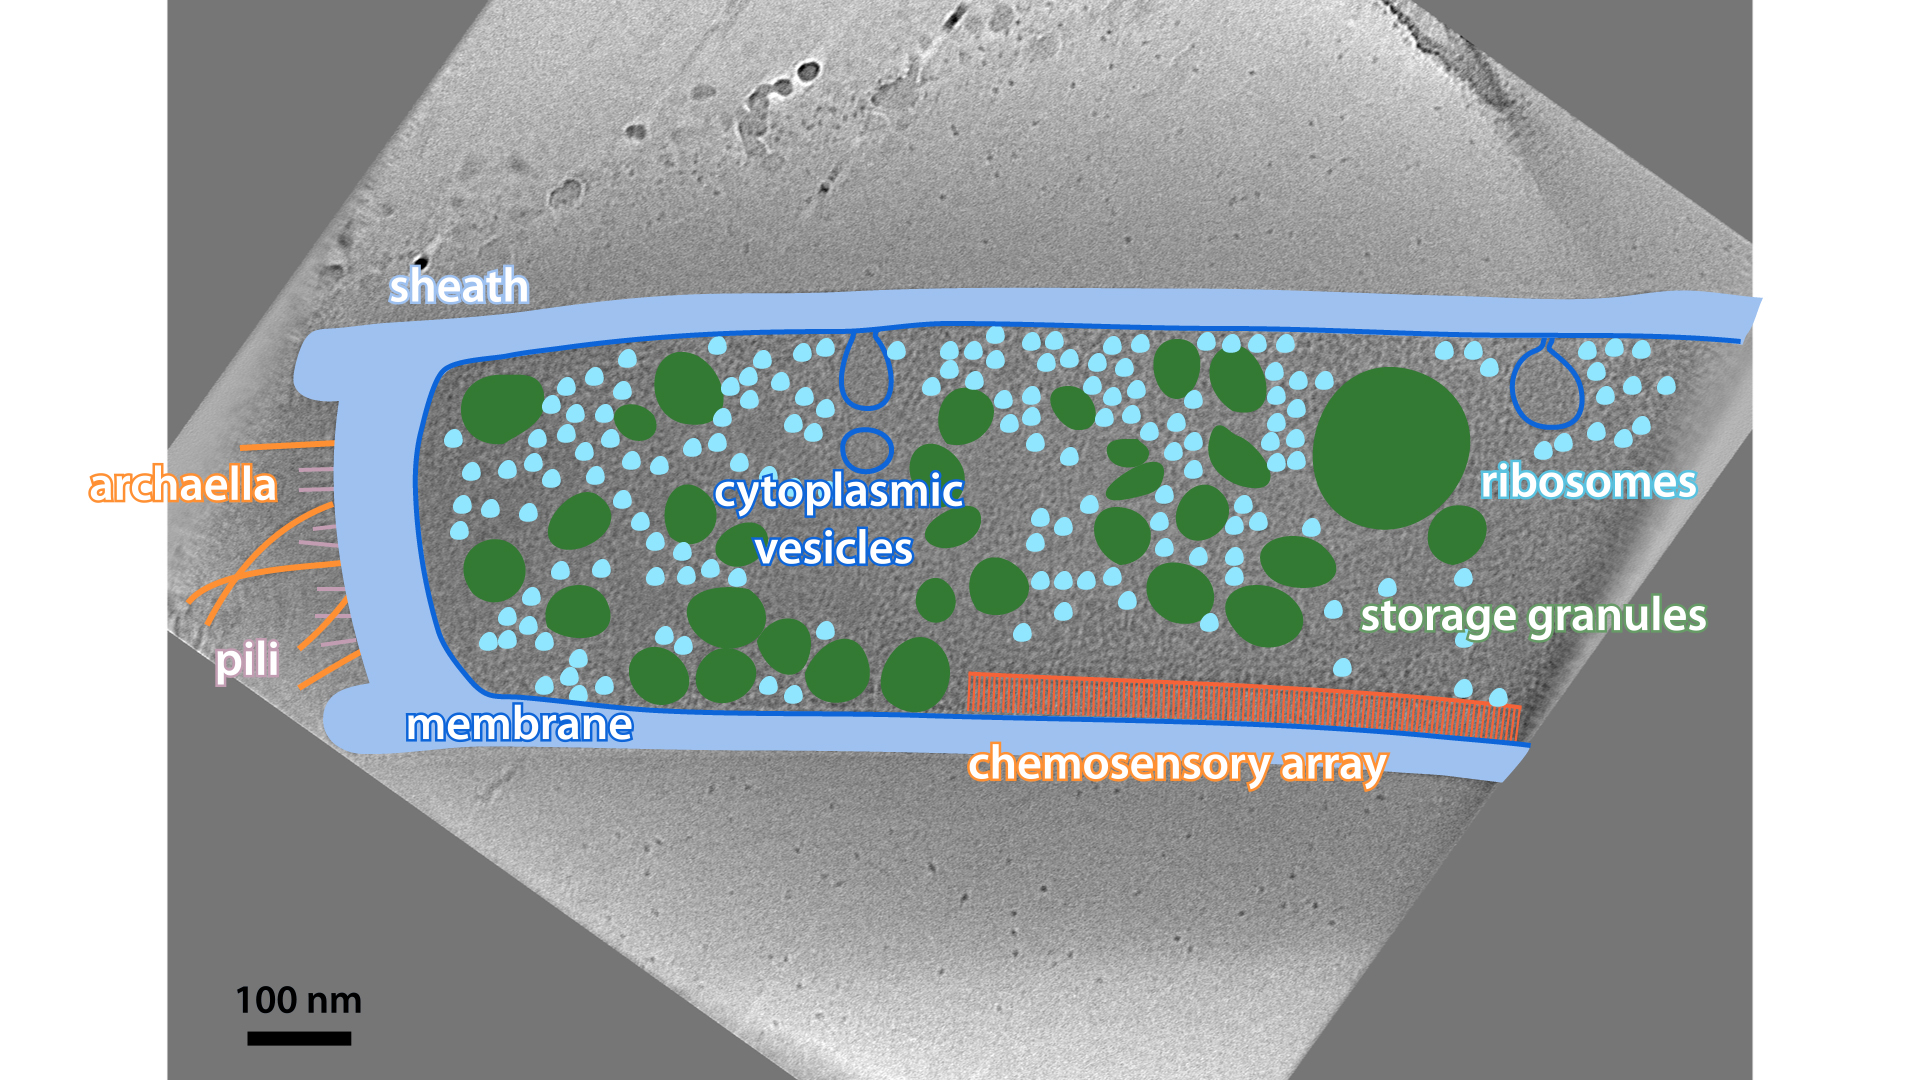
\includegraphics{img/2_8_Mhungatei} \caption[Methanospirillum hungatei Collected by]{Methanospirillum hungatei Collected by: Ariane Briegel [10.22002/D1.1357](https://doi.org/10.22002/D1.1357)}\label{fig:unnamed-chunk-24}
\end{figure}

\section{Haloarcula argentinensis}\label{haloarcula-argentinensis}

All the layers we've just discussed collectively make up the container,
or envelope, of a cell. As you've seen, different species use different
combinations of these components to form their envelopes; the only
constant is the cytoplasmic (or inner, for diderms) membrane. Before we
move on, let's talk briefly about what these envelopes contain. In
addition to water and small molecules, you've already seen some large
protein complexes like motility machineries. You've also seen the
ribosomes -- the protein/RNA complexes responsible for translation. But
you might have been surprised not to see something else: DNA. The
replicating molecule containing the instructions for the life of the
cell is of paramount importance but often invisible by microscopy. But
not always.

Thin filaments of DNA, only about 2 nm wide, blend in with the dense
cytoplasm of the cell. When a cell lyses, though, its cytoplasm diffuses
into the environment and the DNA filaments stand out against the
now-much-reduced background. You can get an idea of the sheer abundance
of DNA in a cell from this Haloarcula argentinensis where the envelope
has ruptured and the contents are spilling out.

\begin{figure}
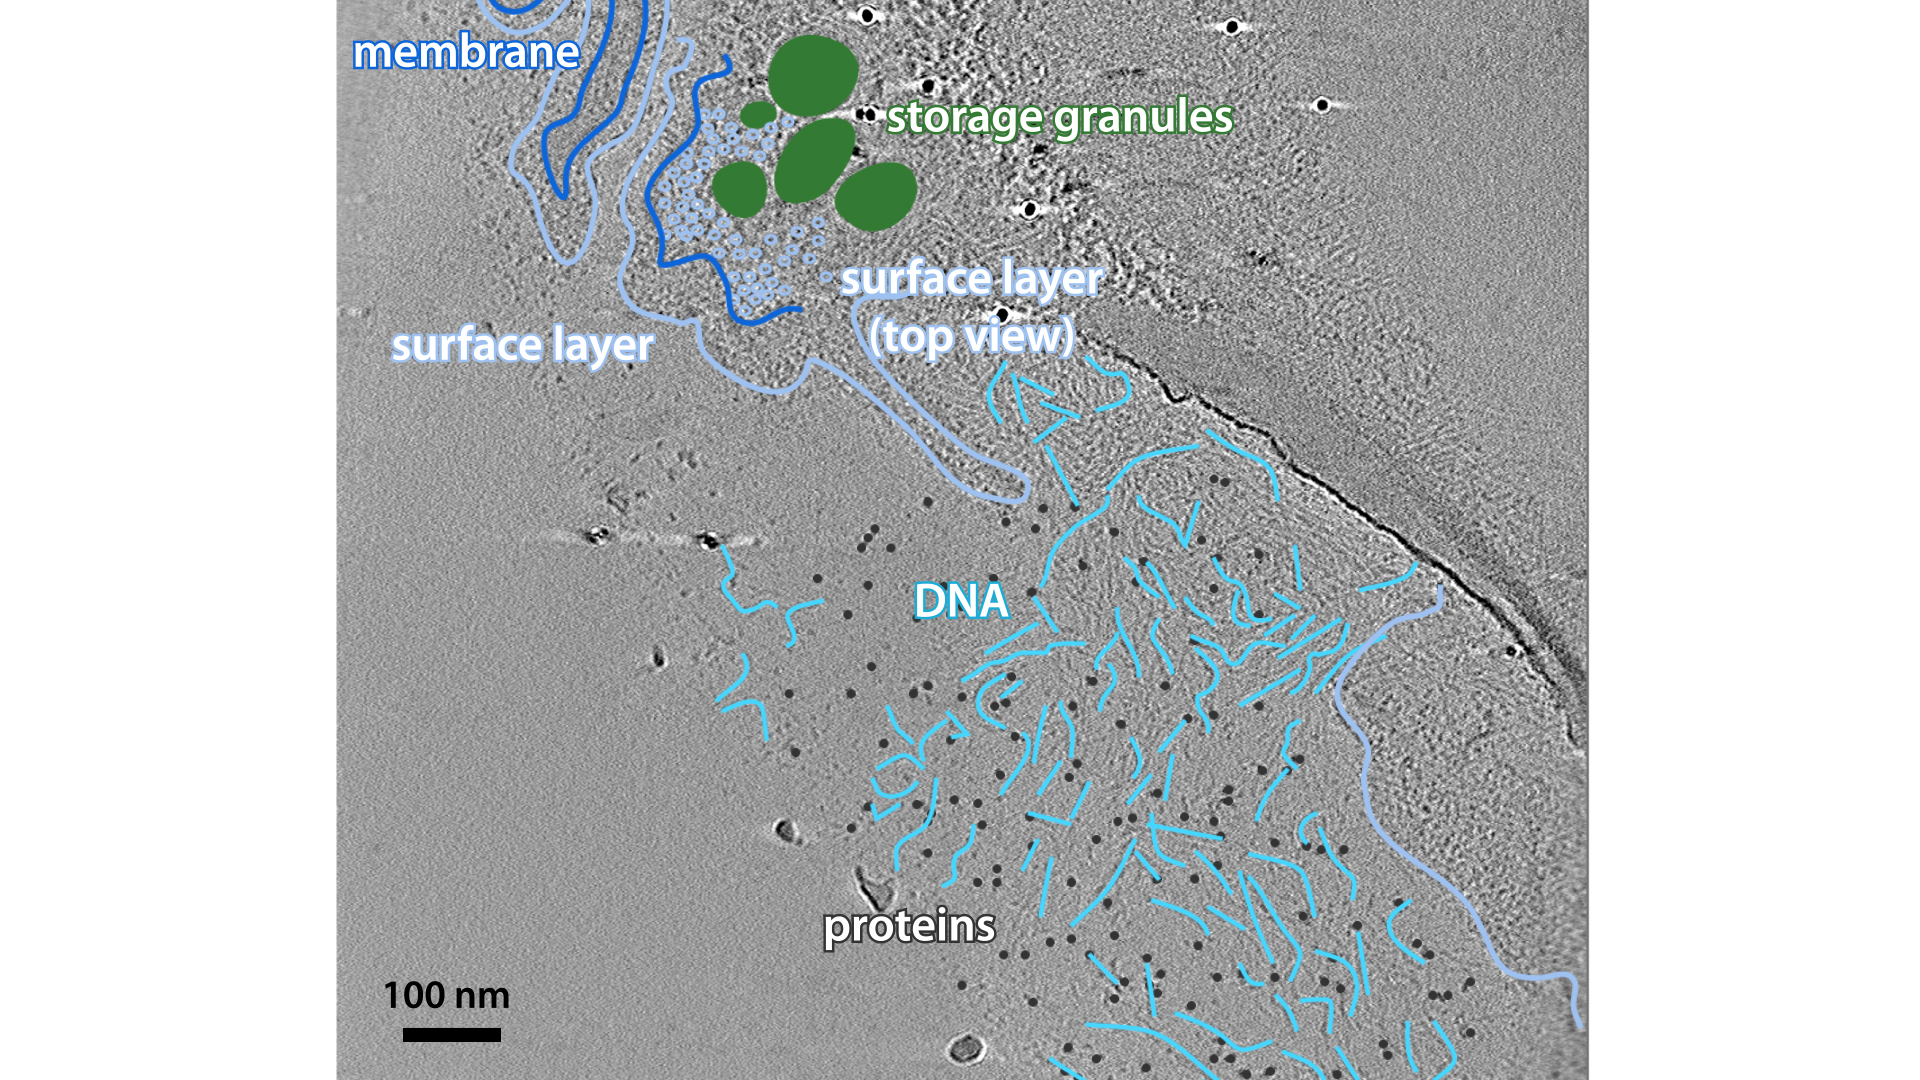
\includegraphics{img/2_9_Hargentinensis} \caption[Haloarcula argentinensis Collected by]{Haloarcula argentinensis Collected by: Ariane Briegel [10.22002/D1.1358](https://doi.org/10.22002/D1.1358)}\label{fig:unnamed-chunk-25}
\end{figure}

\section{Bdellovibrio bacteriovorus}\label{bdellovibrio-bacteriovorus}

Cells contain enormous amounts of DNA. The single, circular chromosome
of this Bdellovibrio bacteriovorus cell contains 3,782,950 individual
base pairs, which means that if the circle were cut and laid out as a
long piece, it would be about one thousand times longer than the cell
itself. To fit and function inside the cell, the chromosome has to be
extraordinarily organized and packed, a feat we still don't understand.
You can see some of this packing in nearly every cell: the center of the
cell tends to have very few large macromolecular complexes like
ribosomes, because they're excluded by the densely-packed chromosome(s).
Watch out for these ribosome-excluding zones in the rest of the book;
they indicate the location of the bulk of the cell's DNA. Since bacteria
and archaea don't enclose their DNA in a subcellular membrane, we don't
call this region a nucleus (the ``karyon'' that defines eukaryotes).
Instead, we use the term nucleoid to describe the cytoplasmic region
where most of the DNA is concentrated.

At times, the nucleoid becomes easier to see. Imagine that you want to
decrease gene expression in your cell. Don't worry yet about why --
we'll discuss that in Chapter 8 -- for now, just think about how. One
approach is simply to pack the chromosome so tightly that the
transcriptional machinery can't access the genes. That's what this cell
is doing, condensing its nucleoid into a dense twisted braid we can
easily visualize.

\begin{figure}
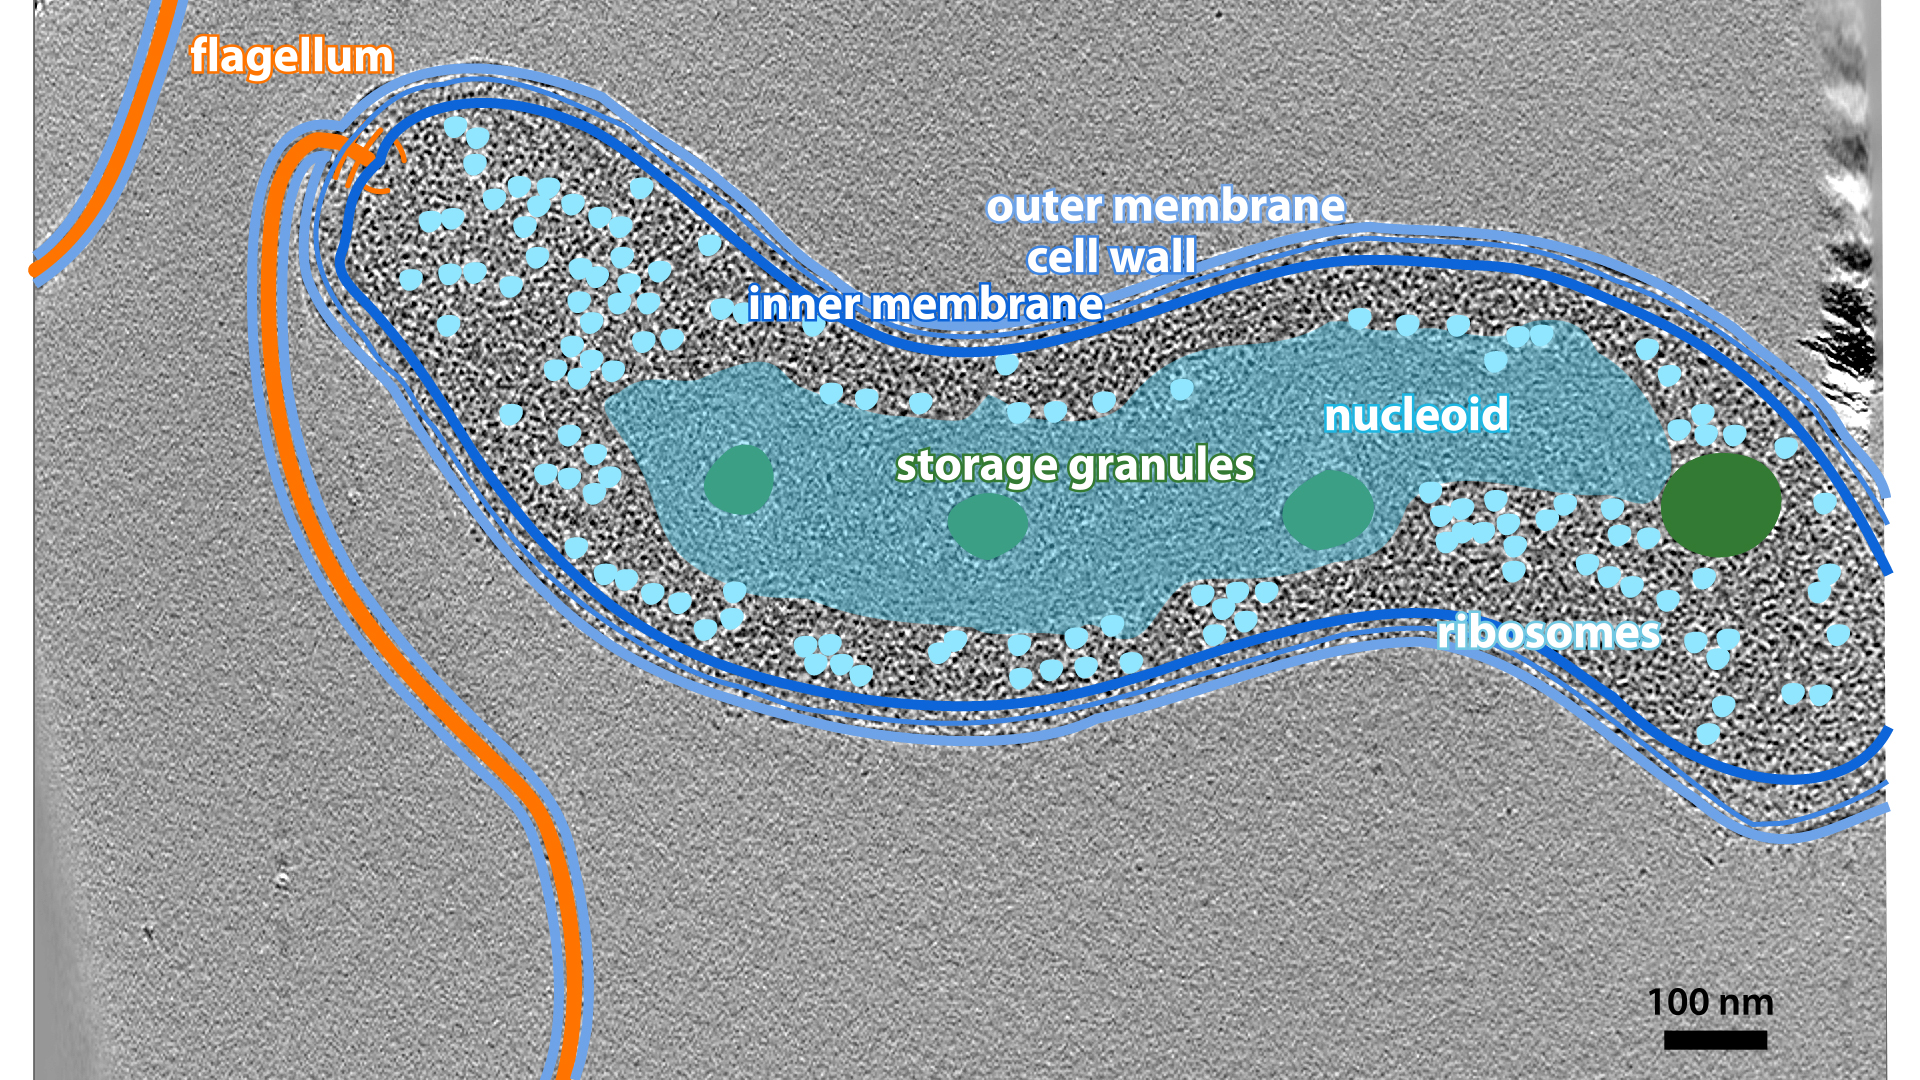
\includegraphics{img/2_10_Bbacteriovorus} \caption[Bdellovibrio bacteriovorus Collected by]{Bdellovibrio bacteriovorus Collected by: Yi-Wei Chang [10.22002/D1.1359](https://doi.org/10.22002/D1.1359)}\label{fig:unnamed-chunk-26}
\end{figure}

\chapter{Shape}\label{shape}

\section{Simkania negevensis}\label{simkania-negevensis}

What kind of life do you envision for your cell? Just as the design of
buildings reflects their purpose, different cell shapes suit different
lifestyles. Does your cell need to soak up sunlight for photosynthesis?
Burrow through tissue? Chase down prey? Each driving function is best
served by a particular form
\protect\hyperlink{Cell_shape_diversity}{Schematic -- Cell shape
diversity}.

How can you give your cell a particular form? The final shape of a
building is determined by a façade erected around a system of internal
beams and joists--its skeleton. Cells determine their shape using a
similar system--the cyto-(``cell'') skeleton--in concert with the rigid
exoskeleton of the sacculus. The cytoskeleton of bacteria and archaea
consists of a set of proteins that form filaments or other
superstructures that move or scaffold other material in the cell. In
many cases, this cytoskeletal scaffolding is dynamic and ever-changing,
appropriate for a living building.

Let's start with a cell like this Simkania negevensis. It's a
sphere--the default shape for a membrane in water, uniformly resistant
to pressure, and the best shape if you want to maximize your volume
relative to surface area. We refer to this spherical shape as coccoid
(``berry-like''). To grow, a coccoid cell can just randomly insert new
glycan strands into its sacculus, expanding into a larger sphere
\protect\hyperlink{Spherical_growth}{Schematic -- Spherical growth}.

\hypertarget{Cell_shape_diversity}{\subsection{Cell shape
diversity}\label{Cell_shape_diversity}}

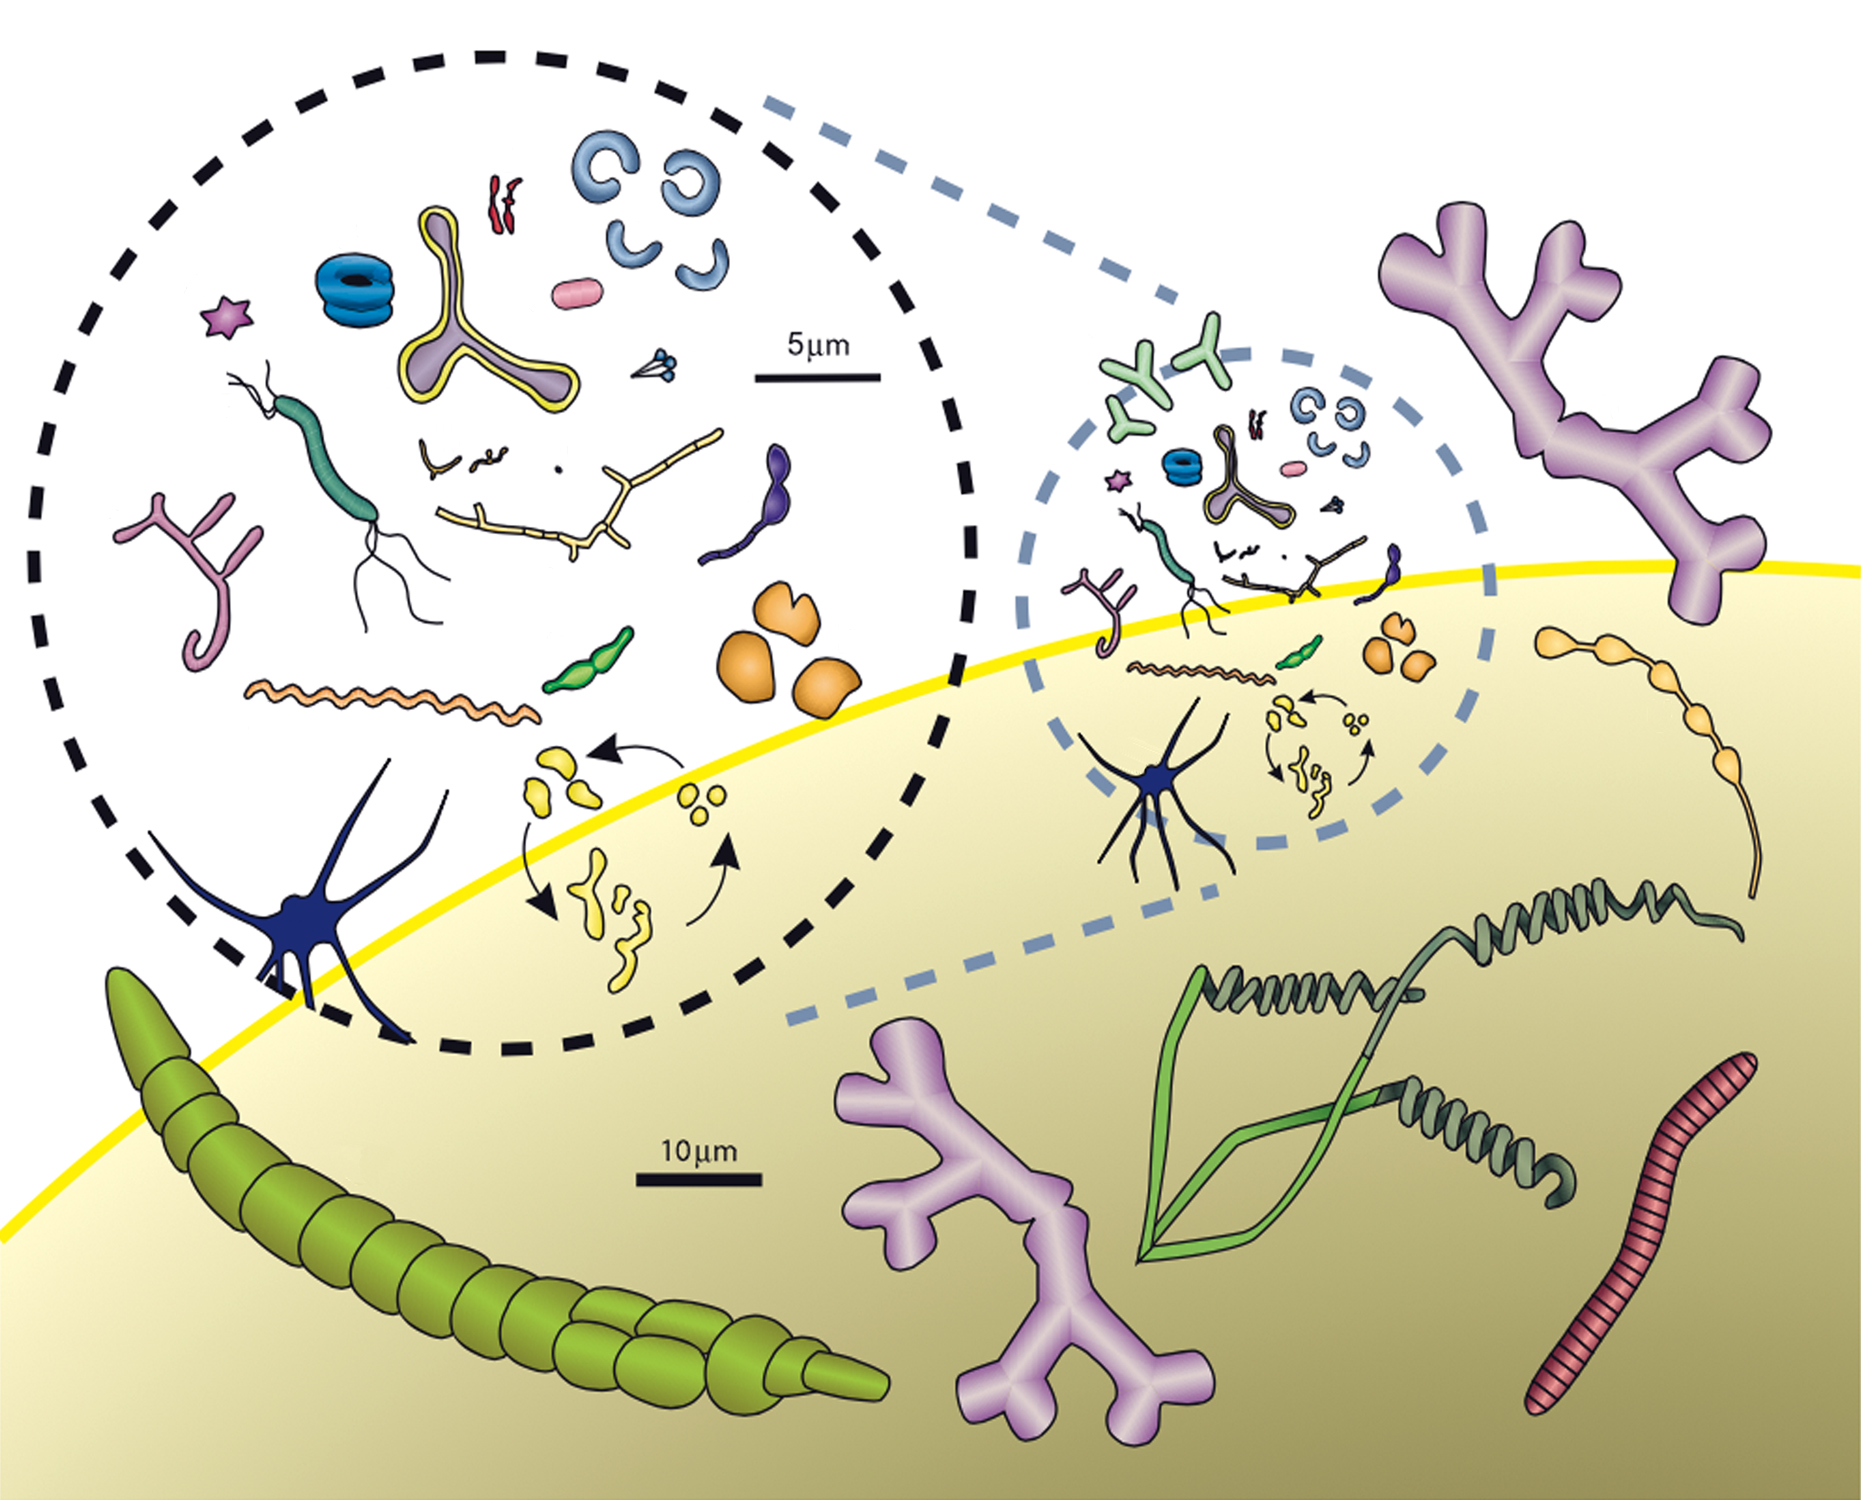
\includegraphics{img/03_schematic/3_1_1_YoungShapes}

Archaea and bacteria adopt a staggeringly diverse set of shapes. Here
are some examples just of bacteria. Note also the range of sizes; what
might at first look like a hill at the bottom is the edge of a cell
drawn to scale.

\hypertarget{Spherical_growth}{\subsection{Spherical
growth}\label{Spherical_growth}}

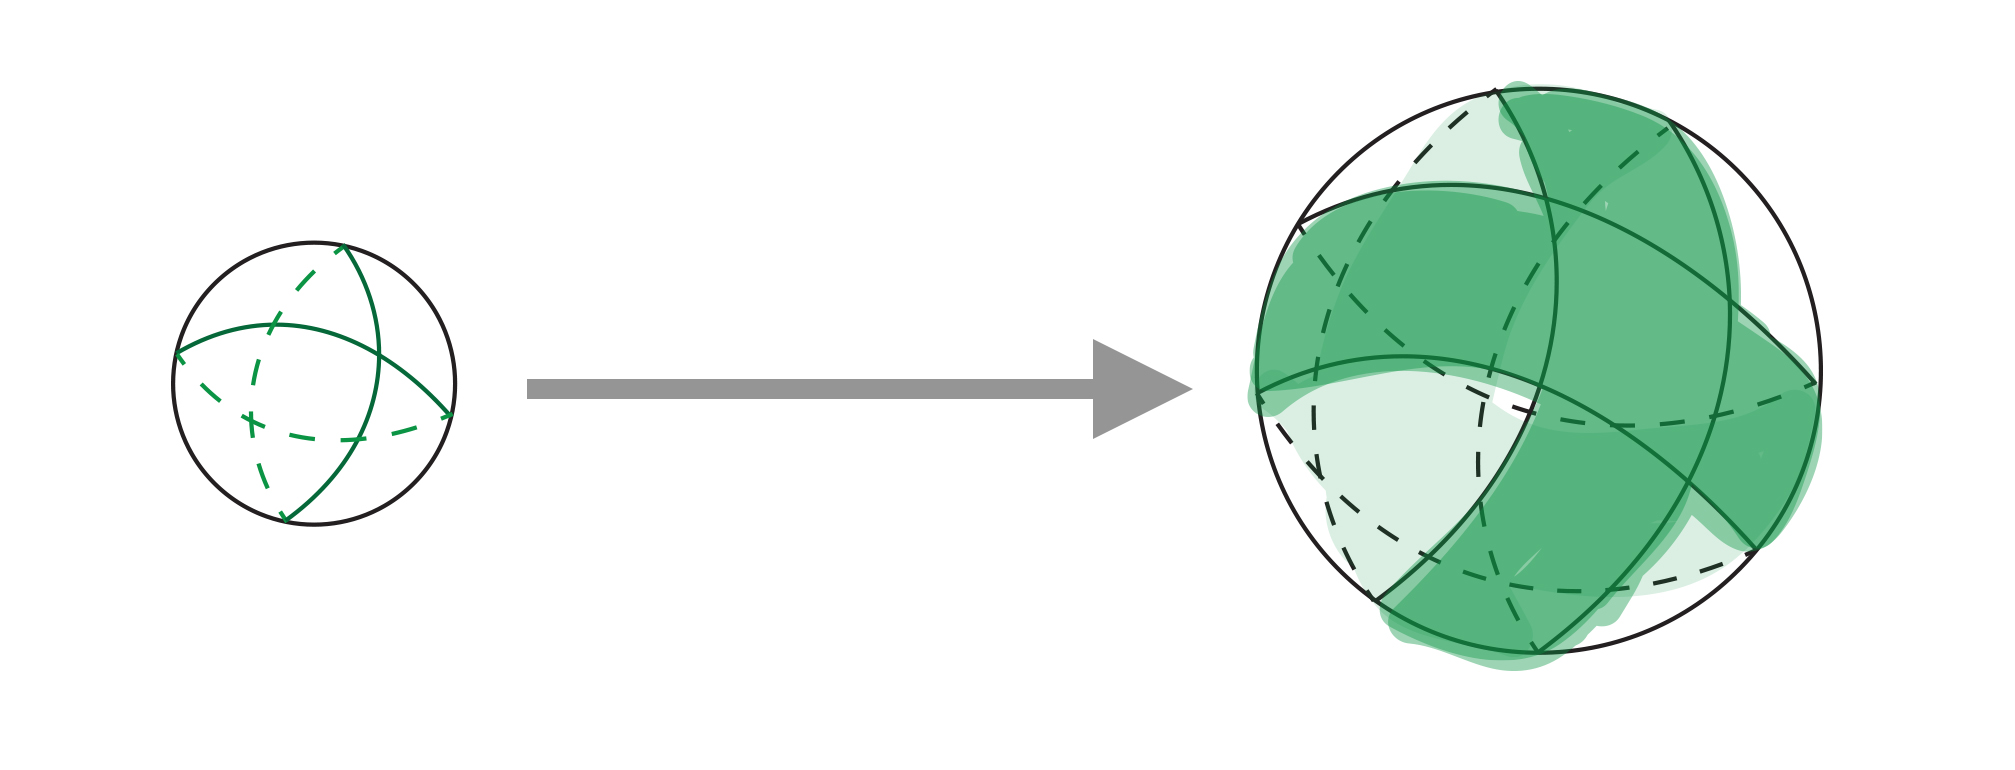
\includegraphics{img/03_schematic/3_1_2_SphericalGrowth}

\section{Cupriavidus necator}\label{cupriavidus-necator-1}

Instead of a sphere, what if you wanted to make your cell cylindrical,
like this Cupriavidus necator? So-called rod-shaped cells (cylinders
with spherical caps) are a very common form for bacteria and archaea,
likely because they're efficient swimmers and swarmers (more on that in
Chapter 6). Starting from a sphere, imagine that you had a construction
contractor who could direct where workers lay in new cell wall. Instead
of random insertion, you could, say, direct them to work around a single
plane. As the workers laid in more and more hoops of peptidoglycan in
this region, a cylinder would form with the same diameter as the initial
sphere (which would now serve as the structure's end caps)
\protect\hyperlink{Rod-shaped_growth}{Schematic -- Rod-shaped growth}.

The contractor for most rod-shaped bacterial cells is a cytoskeletal
protein named MreB (the name reflects the discovery of its gene
neighborhood as a region in which mutations gave E. coli resistance to
the antibiotic mecillinam). MreB is a homolog of the eukaryotic
cytoskeletal protein actin. It's still not clear exactly how it works
(cryo-ET debunked a once-leading theory), but small patches of MreB seem
to shuttle rapidly around the circumference of the cell, directing the
proteins you saw in the last chapter to add new peptidoglycan to the
sacculus. MreB's circuit is restricted to the cylindrical portion of the
cell, expanding the cylinder without affecting the ends. This growth
pattern has an interesting consequence: the peptidoglycan in the cell
caps is older than the peptidoglycan in the cylindrical center. The two
types, old and new, can thus serve as convenient landmarks, allowing the
cell, for instance, to tether something to the end. We'll discuss how
that can be useful in Chapter 5.

Not all rod-shaped bacteria use MreB, and we're still figuring out how
the shape forms in many species {[}More -- Rod variety{]}. For
rod-shaped archaea {[}More -- Archaeal rods{]}, the S-layer is important
for determining shape, but the mechanisms remain unclear.

\hypertarget{Rod-shaped_growth}{\subsection{Rod-shaped
growth}\label{Rod-shaped_growth}}

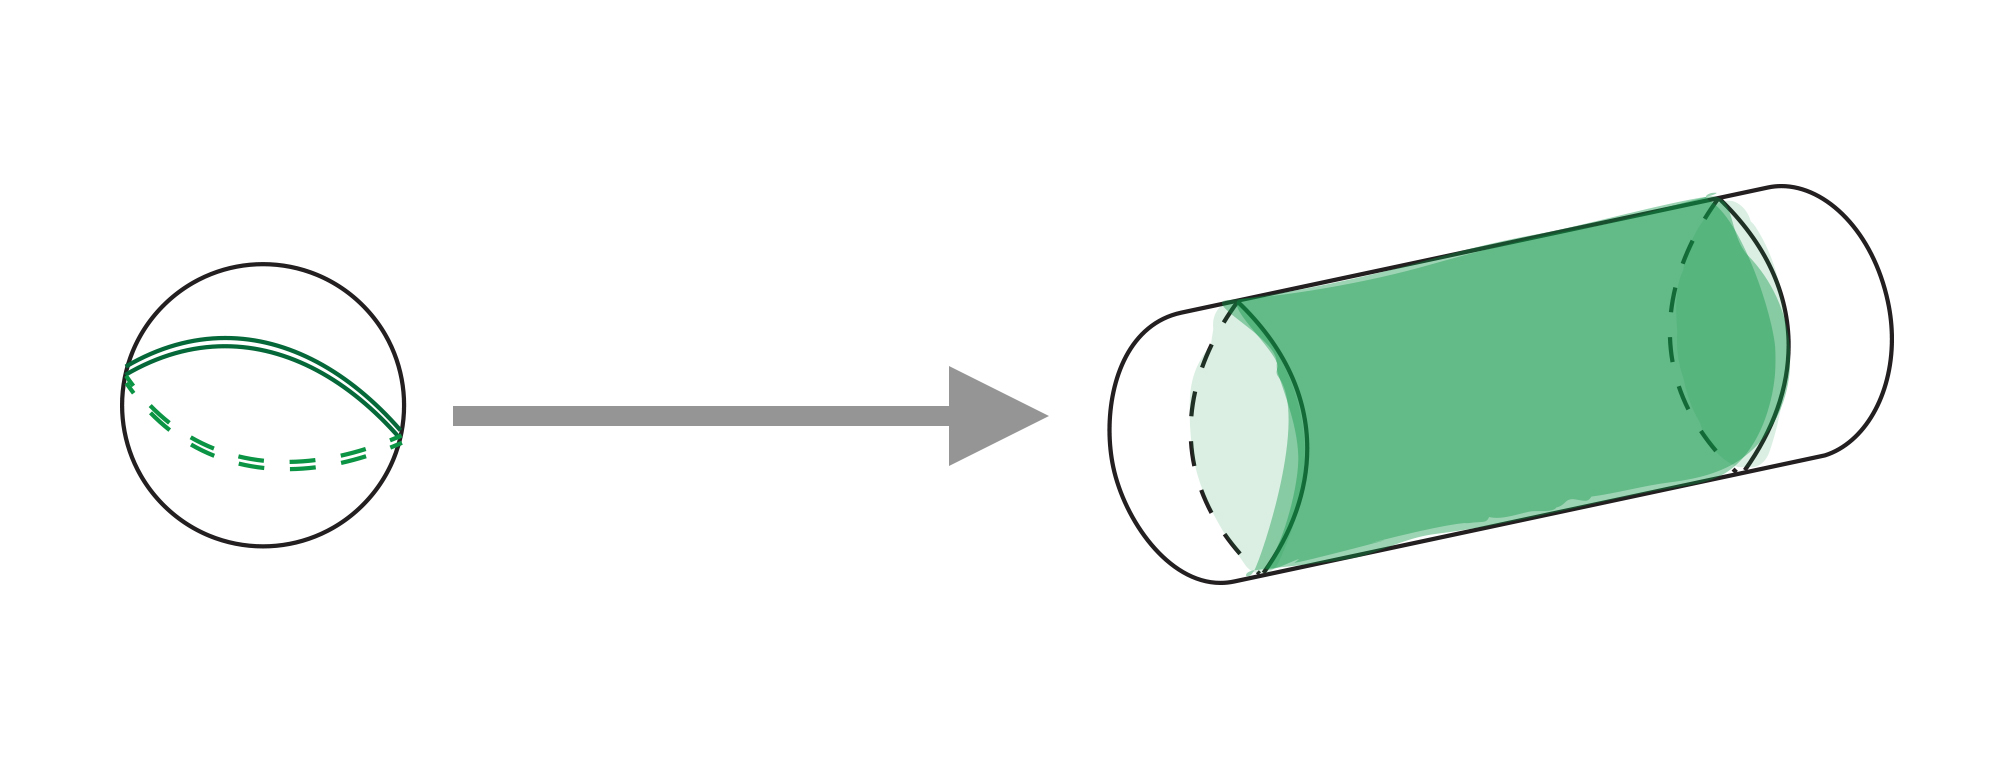
\includegraphics{img/03_schematic/3_2_1_RodGrowth}

\subsection{Brucella abortus}\label{Rod_variety}

Rod-shaped species aren't always perfect rods. For instance, they might
be more pear-shaped, like this Brucella abortus cell. This is one of the
bacterial species that doesn't use MreB.

\subsection{Methanoregula formicica}\label{Archaeal_rods}

\section{Hylemonella gracilis}\label{hylemonella-gracilis}

Rod-shaped cells have a useful property: they can grow by extending
their length without significantly changing the ratio of their surface
area to volume, which would in turn change how efficiently they can take
up nutrients from the environment. This property enables an impressive
range of lengths for rod-shaped cells, from the short C. necator you
just saw, to this much longer Hylemonella gracilis.

The length of a cell (or, more generally, its size) varies depending on
the environment or its stage of the lifecycle. But not that much. Size
tends to be strongly conserved within a species, varying not much more
than the factor of two dictated by division. Sizes between species vary
much more widely, as you'll see throughout the book.

\section{Caulobacter crescentus}\label{caulobacter-crescentus-1}

What if you want to curve your rod-shaped cell into a comma? Vibrioid
shape (named for the genus Vibrio, where it is common) may help cells
swim faster. For Caulobacter crescentus like this one, it can help them
stay close to a surface as liquid flows past, increasing the chance that
their progeny can attach before they're swept away. To make a vibrioid
sacculus, you can imagine the contractor simply telling the workers to
incorporate more material on one side of the rod relative to the other
\protect\hyperlink{Vibrioid_growth}{Schematic -- Vibrioid growth}. This
is the function of a cytoskeletal protein called (for an obvious reason)
Crescentin. Crescentin inhibits cell wall synthesis. It also localizes
to one side of the cell, resulting in more peptidoglycan incorporation
on the opposite side, and a curved cell.

Checks and balances are a common theme in Nature. In this case, a second
contractor makes sure the process doesn't get out of hand. The
cytoskeletal protein CTP synthase inhibits Crescentin, fine-tuning the
process and making sure the cell doesn't curve too much. As its name
implies, CTP synthase has another, metabolic, function in the cell
\protect\hyperlink{CTP_synthase}{Schematic -- CTP synthase}. In C.
crescentus like this, the CTP synthase is easy to see as a bundle of
filaments. Crescentin is more elusive; we only see obvious filaments
when it is artificially overexpressed, so its exact form in the cell
remains unclear.

This system is one way of making a curved cell. There must be others,
though, since many vibrioid species (including Vibrio!) don't use
Crescentin. As you'll see throughout this book, there is no shortage of
biological questions still to figure out.

\hypertarget{Vibrioid_growth}{\subsection{Vibrioid
growth}\label{Vibrioid_growth}}

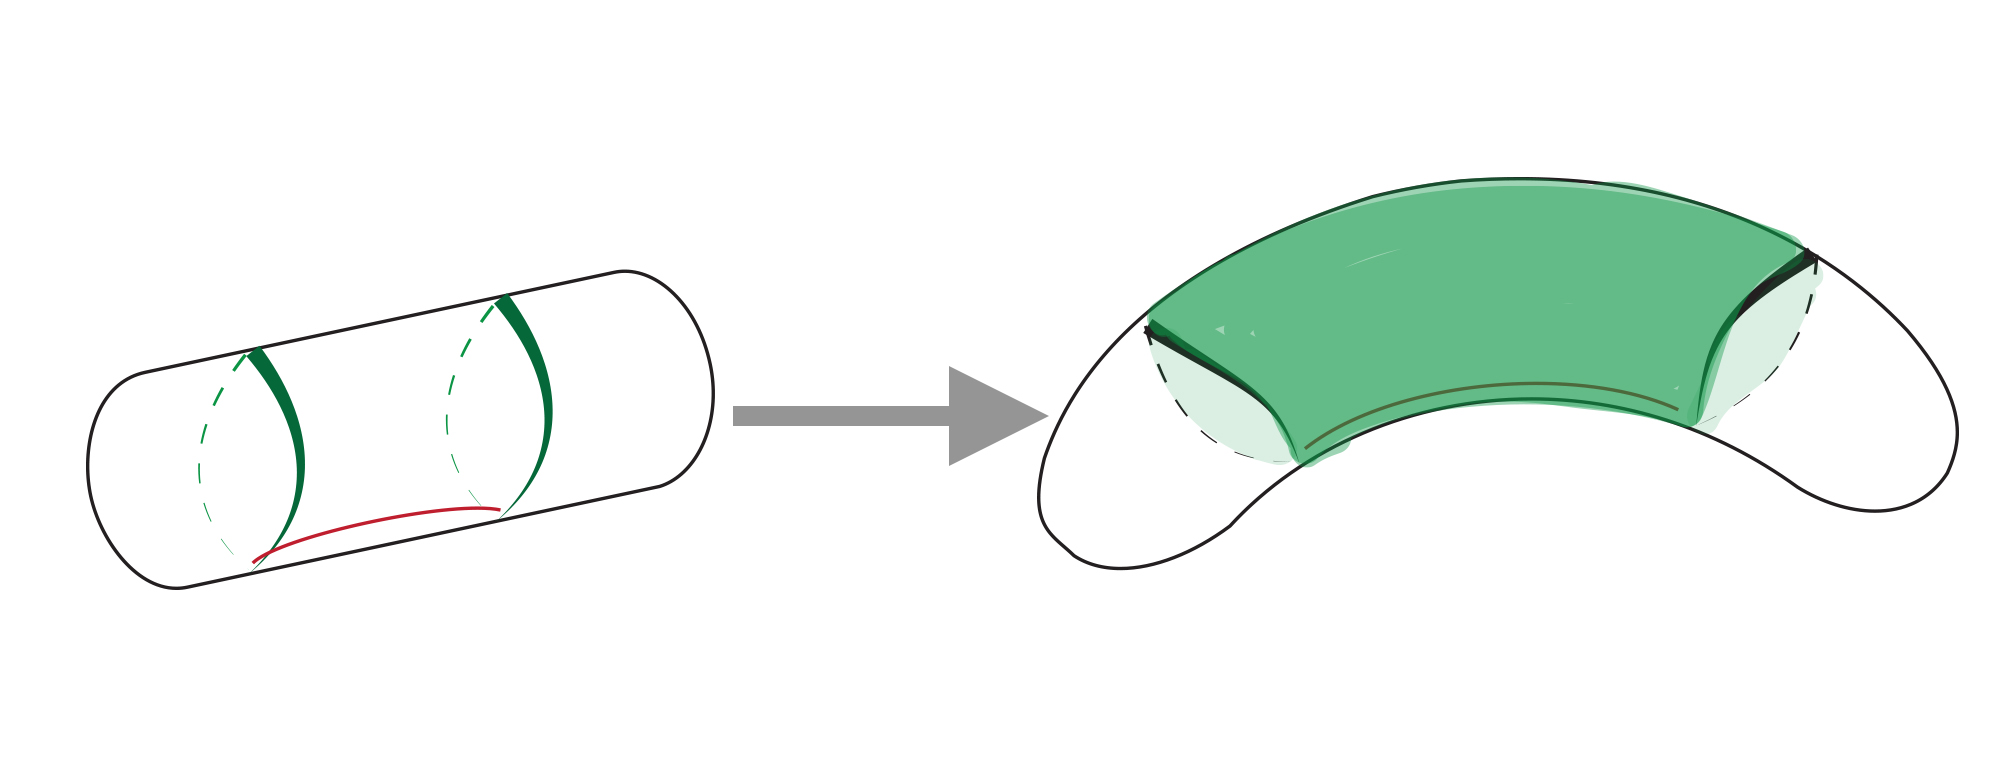
\includegraphics{img/03_schematic/3_4_1_VibrioidGrowth}

\hypertarget{CTP_synthase}{\subsection{CTP
synthase}\label{CTP_synthase}}

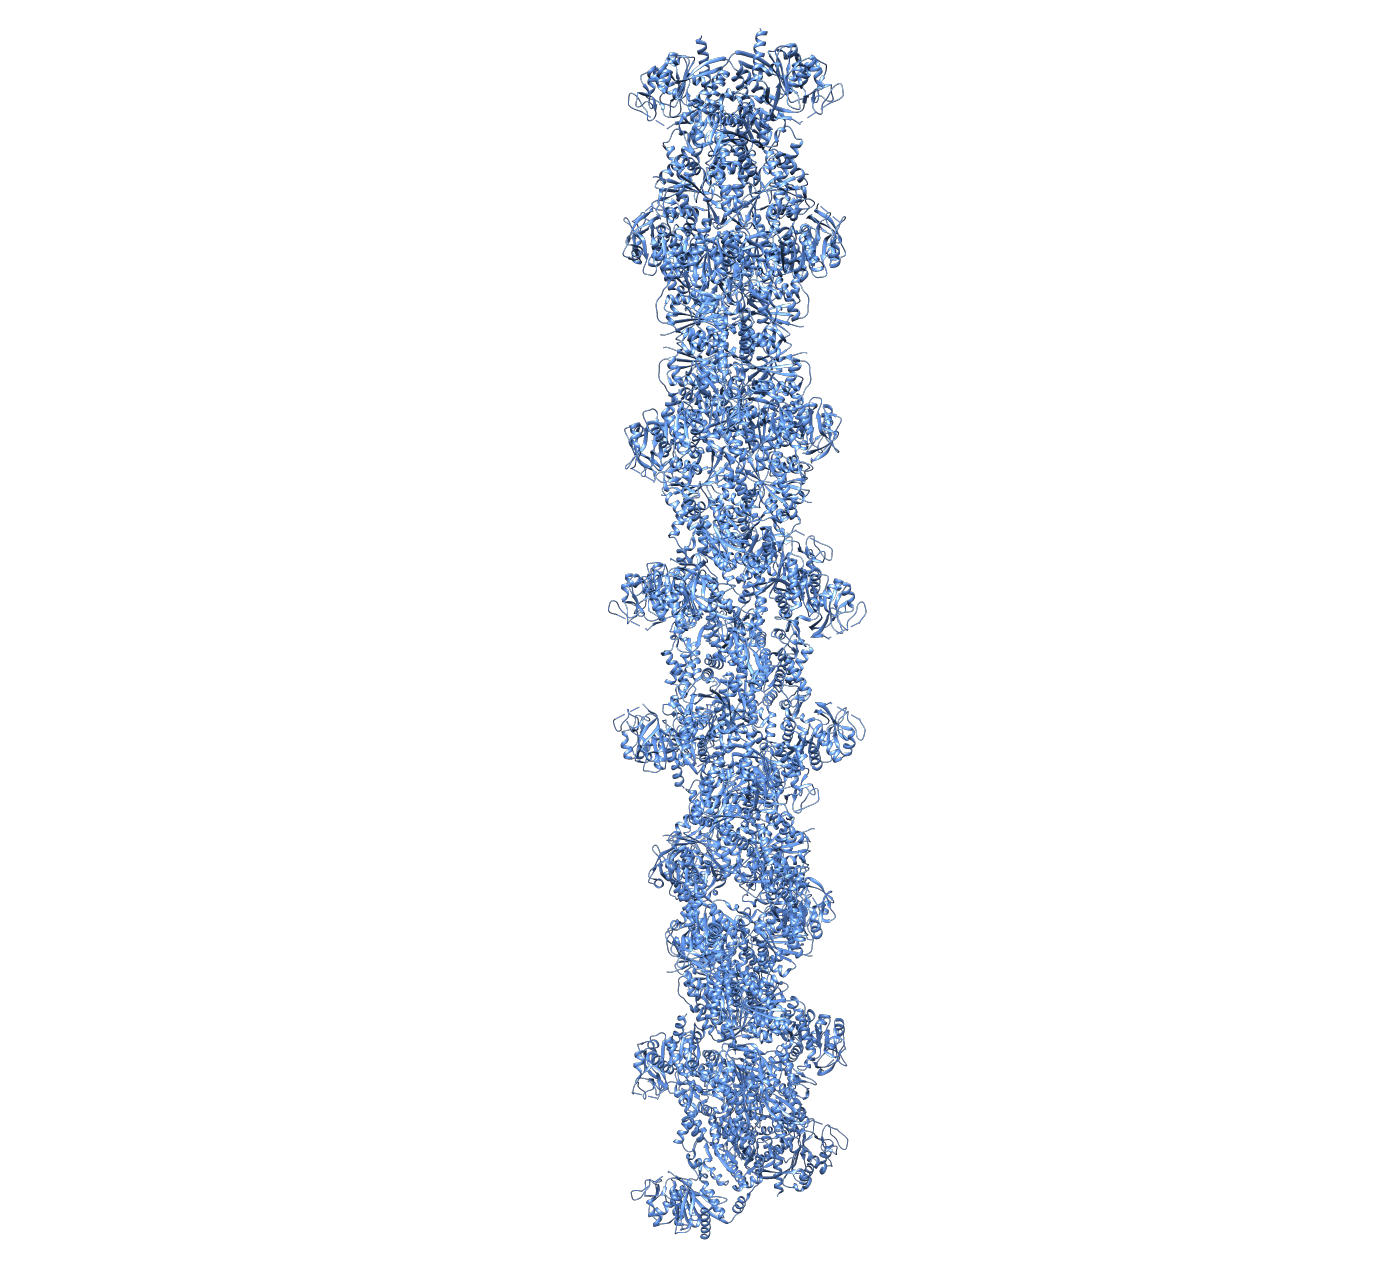
\includegraphics{img/03_schematic/3_4_2_CTP_synthase}

CTP synthase is a fundamental metabolic protein across all domains of
life, helping make the building blocks of RNA and DNA. It is also not
the only metabolic protein seen to form filaments in bacteria and
archaea. This suggests that polymerization might be serving another
role, perhaps as a way to regulate the activity of an enzyme that may
not always be needed, but would be costly or slow to degrade and
synthesize again. In that case, the cytoskeletal role may have arisen
secondarily; once you have a long filament lying around, why not use it
as scaffolding?

\section{Campylobacter jejuni}\label{campylobacter-jejuni}

Why stop at a quarter turn when you can twist your cell into a full wave
or even a corkscrew? Just as the corkscrew penetrates its target,
helical pathogenic bacteria like this Campylobacter jejuni can burrow
efficiently into the tissue of their target. More on that in Chapter 6.
For now, let's just consider how these shapes can be formed.

It's tempting to group species with a common characteristic, but
appearances are often deceiving about relatedness. Helical shape, for
instance, was not a one-shot invention; it was invented independently
multiple times. This is true of other bacterial and archaeal cell shapes
as well. For helical shape, these independent origins are reflected in
diverse mechanisms of creating it. Some species, like C. jejuni, use
dedicated proteins to regulate the pattern of peptidoglycan insertion--a
continuation of the theme we've been discussing. Other species take
different approaches {[}More -- Borrelia burgdorferi{]}.

\subsection{Borrelia burgdorferi}\label{Borrelia_burgdorferi}

Borrelia burgdorferi like this cell use the long filaments of their
motility machinery (flagella, discussed in Chapter 6) as a kind of
cytoskeleton. A bundle of flagella wraps around the cell in the
periplasm, between the sacculus and the outer membrane. As motors at
their base spin them, these filaments impart a helical wave pattern to
the sacculus; without their rotation the cells develop a rod shape. B.
burgdorferi aren't actually helical; rather they are wave-shaped, a
2-dimensional curve instead of a 3-dimensional one.

\section{Verrucomicrobium spinosum}\label{verrucomicrobium-spinosum}

Motility isn't everything. Another major force shaping cells is
metabolism. Nutrients are often scarce, and increasing your cell's
ability to absorb them can give it a boost in the competitive game of
life. So how can you do that? Remember that a sphere maximizes volume
relative to surface area. To maximize surface area (for nutrient uptake)
relative to volume, you'd want something spikier. Some bacteria extend
prosthecae (``add-ons'' or appendages) for this purpose. Some, like
Caulobacter crescentus, use a single prostheca, which is also called a
stalk. Stalks are commonly located at the end of the cell, where, as
you'll see in Chapter 8, they can help attach the cell to a surface,
letting them hang on even in turbulent flow in the freshwater lakes and
streams where they live. Other species have a stalk on either end. Still
others, like this Verrucomicrobium spinosum, form astral shapes with
prosthecae jutting out in all directions.

Prosthecae offer a challenge for the architect: thin extensions are
delicate. Prosthecate cells use cytoskeletal proteins to form and
stabilize their stalks, although exactly how this works remains unclear.
One of these cytoskeletal proteins is Bactofilin
\protect\hyperlink{Bactofilin}{Schematic -- Bactofilin}, which is
similar to the proteins that make intermediate filaments in eukaryotes.
C. crescentus use Bactofilin polymers to help make their stalks.
Prosthecobacter contain microtubules {[}More -- Bacterial
microtubules{]} in their stalks, but their function remains unclear.

\hypertarget{Bactofilin}{\subsection{Bactofilin}\label{Bactofilin}}

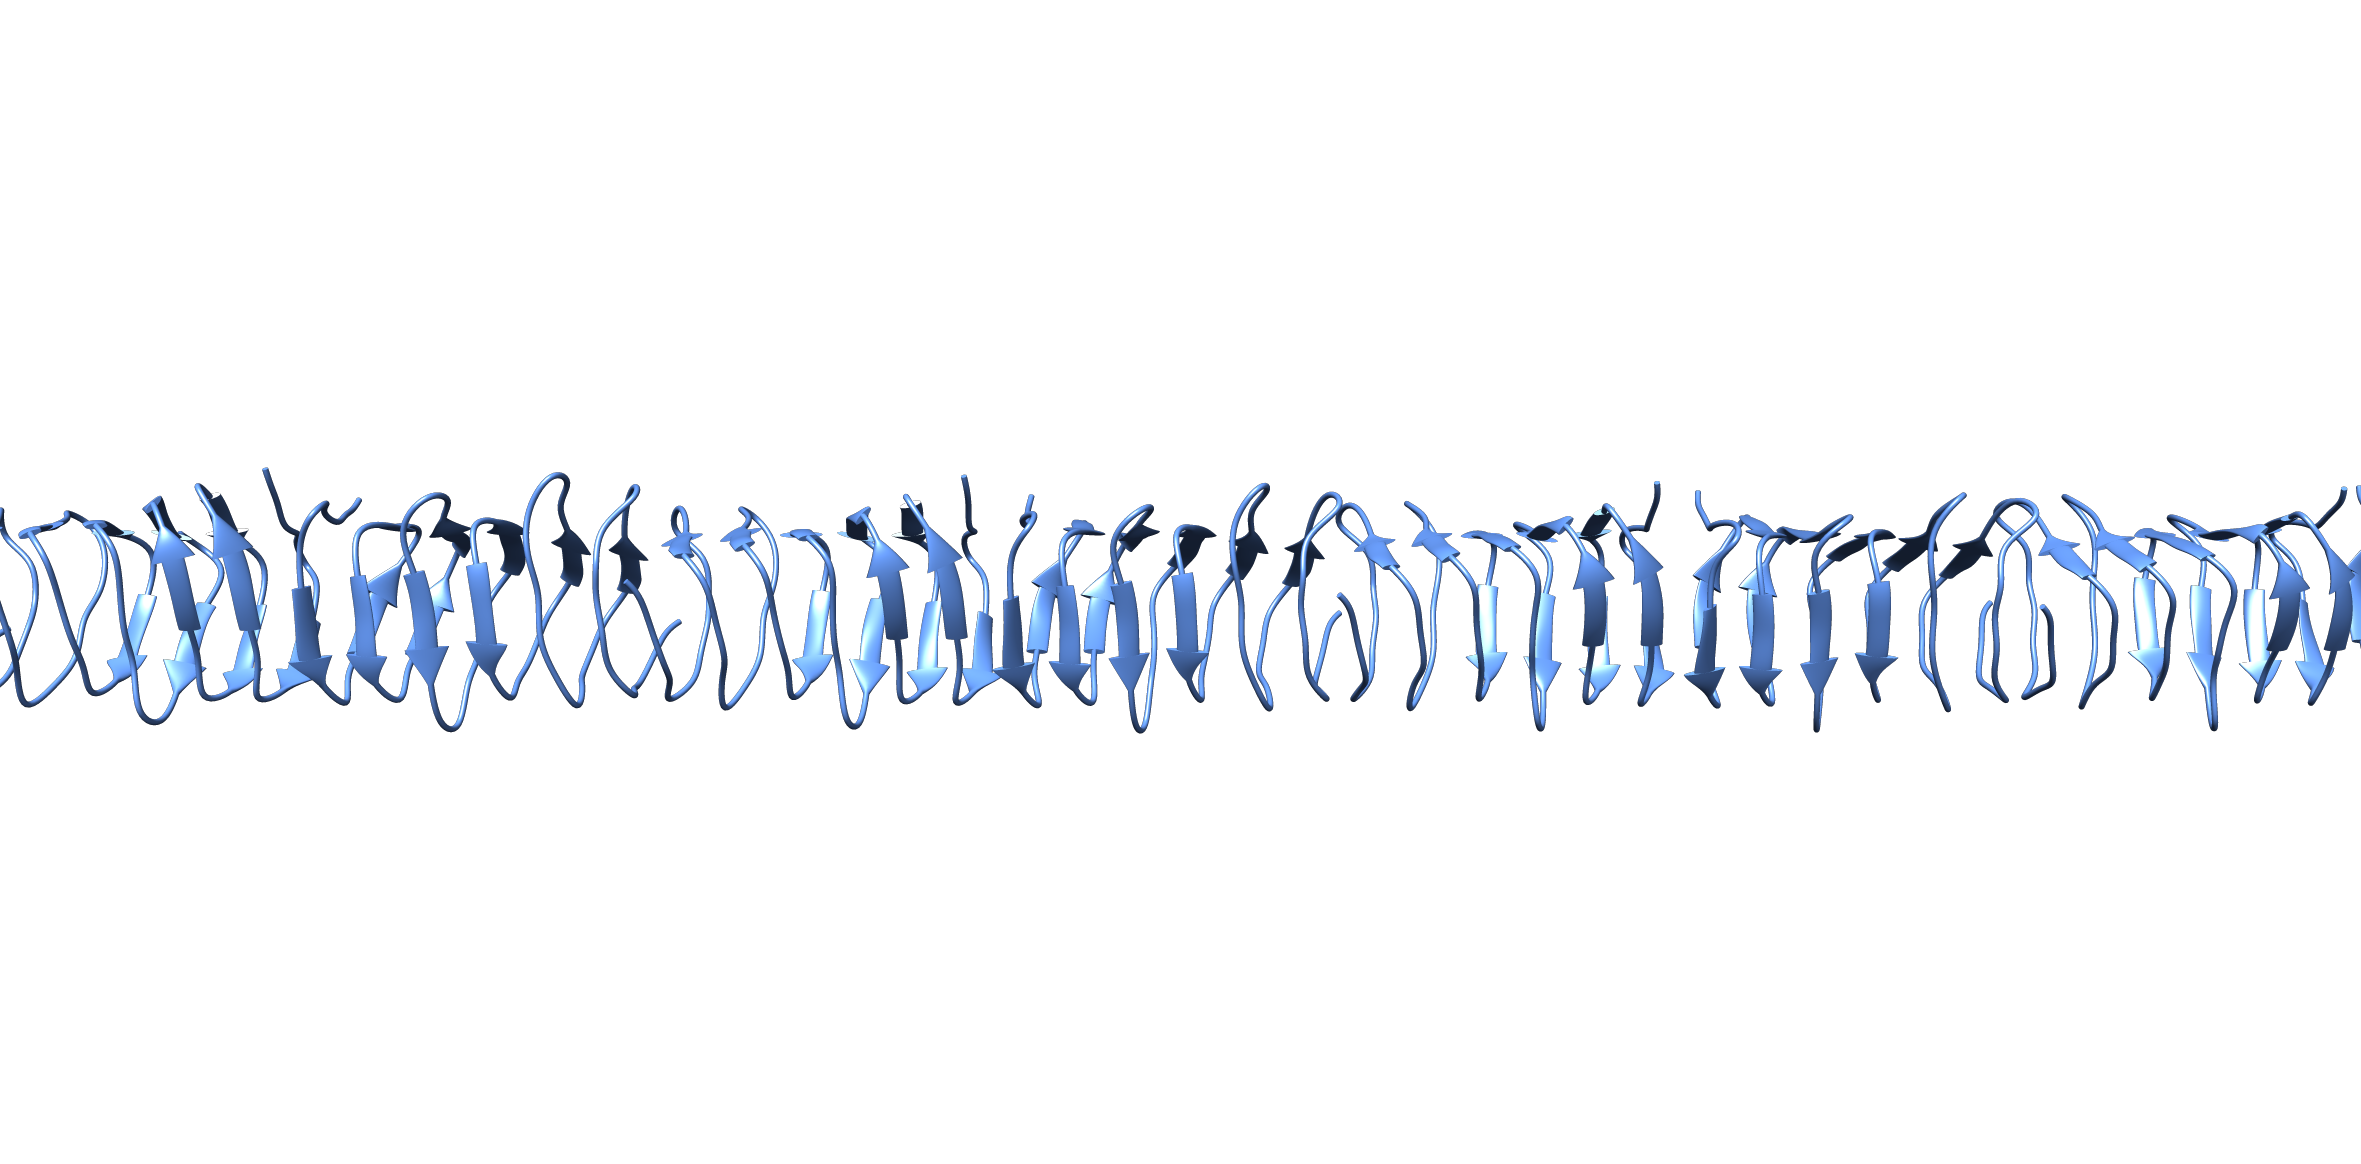
\includegraphics{img/03_schematic/3_6_1_bactofilin}

\subsection{Prosthecobacter vanneervenii}\label{Bacterial_microtubules}

Some bacterial species with prosthecae express structures similar to
eukaryotic microtubules, made from two proteins called BtubA and BtubB
to reflect their homology to eukaryotic tubulins. Eukaryotic
microtubules are hollow tubes formed by 13 protofilaments; bacterial
microtubules are smaller, with only \textasciitilde{}5 protofilaments.
Cells commonly contain a bundle of microtubules in their prostheca, like
this Prosthecobacter vanneervenii cell, which has a bundle of four.

Prosthecobacter belong to an evolutionarily unique group of species that
share characteristics unusual in the rest of the bacterial phylogenetic
tree. We refer to the collective group as the PVC superphylum (because
it contains Planctomycetes, Verrucomicrobia, and Chlamydiae). Having
homologs of eukaryotic microtubule proteins is one of these unique
characteristics; so far, Btubs have only been identified in species of
Prosthecobacter. They seem to have come from a horizontal gene transfer
from a eukaryotic cell (meaning that microtubules evolved first in
eukaryotes and were later borrowed by the bacteria).

\section{Haloquadratum walsbyi}\label{haloquadratum-walsbyi}

All the cells whose shape we've discussed so far have been bacteria, but
archaea hold their own in the specialized shape competition. In fact,
one of the most extreme examples of maximizing surface area relative to
volume comes from this archaeon, Haloquadratum walsbyi, which grows as
thin, square tiles. Very thin, square tiles. This property helps keep
them oriented with their broad sides to the sun, whose light they
convert to energy. They divide in this plane, too, with their progeny
extending the sheet of tiles. Gas vesicles {[}More -- Gas vesicles{]}
keep the cells buoyant in the super-salty lakes where they live.

It's still not exactly clear how this shape is determined, but at least
part of the mechanism seems to involve glycoproteins on the cell
surface.

\hypertarget{Gas_vesicles}{\subsection{Halobacterium
salinarum}\label{Gas_vesicles}}

Some species of archaea and bacteria use gas vesicles to control their
buoyancy. This can allow them to rise or fall in a water column, which
can be a great advantage. Halobacterium salinarum like this one produce
gas vesicles in response to cues from the environment, lifting
themselves out of the sediment and into more favorable conditions of
oxygen or sunlight for photosynthesis. This cell has just started
producing gas vesicles, so they are small and isolated. Later, the
vesicles will elongate into cylinders with conical ends
\protect\hyperlink{Gas_vesicles}{Schematic -- Gas vesicles}. Each cell
might contain dozens of vesicles, and they often cluster together.

\hypertarget{Gas_vesicles}{\subsection{Gas
vesicles}\label{Gas_vesicles}}

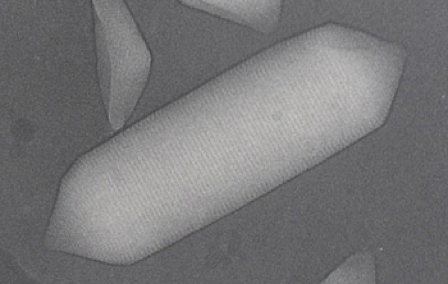
\includegraphics{img/03_schematic/3_7_1_GasVesicle}

Gas vesicles are microcompartments enclosed by a hydrophobic shell made
of a single layer of protein. (Sometimes additional proteins reinforce
the shell.) Gas vesicles don't actually store gas; they simply allow gas
dissolved in the cytoplasm to diffuse in, while forming a tight barrier
against anything else, like water. They are sensitive and prone to
collapse with even a slight increase in the surrounding pressure.

\chapter{Growth}\label{growth}

\section{Caulobacter crescentus}\label{caulobacter-crescentus-2}

The life of a cell is simple in theory, and complex in practice. Think
about the evolutionary purpose of your cell. Fundamentally, it is to
grow, amassing enough resources to eventually multiply itself. How best
to grow, though, depends on the environment and what's available to use
as fuel. Different species have evolved different strategies to optimize
their growth. In a world of scarce resources and fierce competition, any
adaptation that lets your cell grow more efficiently can have a big
effect on its success. Often these adaptations are visible in the
structure of the cell, as you'll see in this chapter.

You've already seen how the shape of your cell can allow it to gather
nutrients from the environment more efficiently. For example,
Haloquadratum walsbyi uses a flat shape to maximize its exposure to
sunlight for photosynthesis. Alternatively, prosthecate bacteria like
Caulobacter crescentus use long, thin extensions to increase surface
area relative to volume, allowing them to absorb more nutrients. Let's
examine these extensions more closely.

The extra surface area of a stalk can increase your cell's ability to
absorb nutrients, but it also adds a lot of membrane that can dilute
membrane proteins and increase the time it takes them to diffuse around
the cell. C. crescentus stalks get longer throughout their lifetime, so
the problem only gets worse with age. As an engineer, how could you
solve this problem? What if you could separate the envelope of the stalk
from the envelope of the rest of the cell? C. crescentus cells like this
one have evolved an elegant way of doing this: stalk bands. These
protein structures form diffusion barriers for the membranes and
periplasm, but not the cytoplasm. Each cell division produces another
band in the elongating stalk, so you can tell a cell's age by counting
its bands.

{[}2\_Shewanella oneidensis{]}

Other cell extensions also help metabolism. Non-photosynthetic cells
break down nutrients into chemical energy (ATP) through respiration
reactions. The chemistry is beyond the scope of this book, but it
involves the transfer of electrons to an acceptor molecule, typically
oxygen (the ``aer'' in aerobic respiration). When oxygen isn't present,
some cells can use an alternative electron acceptor, such as iron or
sulfur, in a process called anaerobic respiration. This works well when
the acceptor is soluble and can diffuse into the cell. But what if the
only available acceptor is trapped in a mineral? Shewanella oneidensis
like this one have evolved a workaround: they extend outer membrane
vesicle chains. Electron carriers in the membrane
\protect\hyperlink{Cytochromes}{Schematic -- Cytochromes} shuttle
electrons to metal oxide minerals in the environment, a conductive
property that lends the appendages the name ``nanowires.'' The
morphology of S. oneidensis nanowires is similar to that of other outer
membrane vesicle chains, with tubular and pearled sections. Here the
nanowire has detached from the cell. You can also see metal deposits on
the cell's envelope, which it is presumably using for respiration.

Other species, like Geobacter sulfurreducens, also use nanowires to
transfer electrons to an insoluble acceptor in the environment, but the
structure of these nanowires is very different: a long filament made
from stacked cytochrome proteins, resembling a pilus (thin protein
filaments you'll see in Chapters 6 and 9).

4\_2\_1 Schematic: Cytochromes

This model shows the arrangement of cytochromes (red and green dots) on
the section of S. oneidensis nanowire you saw on the main page. The
membrane is colored in gold.

\section{Rhodopseudomonas palustris}\label{rhodopseudomonas-palustris}

What if your cell gathers energy from sunlight; how can you make that
process more efficient? Photosynthetic bacteria harvest light energy
using protein complexes \protect\hyperlink{Photocomplexes}{Schematic --
Photocomplexes} embedded in their membranes. It seems intuitive to
increase the light-gathering capability of such a cell by adding more
membrane. But then the cell's volume would also increase. How could you
get around this problem? Why not stack the extra membrane in the
cytoplasm? Many (but not all) photosynthetic bacteria contain
intracytoplasmic membrane, or ICM. In cells like this Rhodopseudomonas
palustris, the ICM is continuous with the inner membrane and forms
stacks at the middle of the cell. Different species can have different,
and more extensive, arrangements {[}More -- ICM variety{]}.

4\_3\_1 Schematic: Photocomplexes In the ICM, the light-harvesting
photocomplexes are themselves highly organized. As you can see here, the
complexes comprise hundreds of individual proteins and can reach tens of
nanometers in size. Physically tethering enzymes that function in the
same pathway increases efficiency by allowing the enzymes that catalyze
subsequent steps to hand off substrates. You'll see more examples of
this theme in the rest of the chapter; metabolic enzymes in the cell are
often clustered together into relay teams.

\subsection{Methyloprofundus sedimenti}\label{ICM_variety}

In some species, like this Methyloprofundus sedimenti, the ICM is even
more extensive and appears to be fully separated from the cell membrane.
As you can see, it occupies much of the cytoplasmic space.

\section{Chloroflexi}\label{chloroflexi}

Another approach to accommodate additional enzymatic workers is to put
them in a dedicated factory. Rather than extending their membranes, some
bacteria, like this Chloroflexi, use dedicated structures called
chlorosomes to pack together many light-harvesting complexes. This
approach of bringing together enzymes that function in the same
metabolic pathway is a common way cells increase efficiency.

\section{Thiomonas intermedia}\label{thiomonas-intermedia}

You might be able to increase the efficiency of your factory even
further by enclosing it in a dedicated building. Many bacteria (but not,
as far as we know, archaea) do this by forming microcompartments--areas
of the cytoplasm walled off by a protein shell
\protect\hyperlink{Microcompartment_shells}{Schematic --
Microcompartment shells}. One of the most impressive microcompartments
is the carboxysome that some bacterial species use for carbon fixation
(the breakdown of carbon dioxide into usable fuel molecules).
Carboxysomes contain tightly packed copies of an enzyme called ribulose
bisphosphate carboxylase/oxygenase, or more simply, RuBisCO, which,
incidentally, is the most abundant enzyme on Earth. The shell does more
than simply concentrate the enzymes. Oxygen competes with carbon dioxide
for binding RuBisCO, so the bacteria include another enzyme in the
compartment which converts bicarbonate into CO2, making it readily
available to the RuBisCO. The shell may also slow down the diffusion of
CO2 out, and O2 in. Carboxysomes probably weren't necessary in early
cells because the oxygen level of the environment was much lower. Cells
like this Thiomonas intermedia contain many carboxysomes. While most are
icosahedral, there is variation in their forms {[}More -- Carboxysome
variety{]}.

Microcompartments can protect their contents from the rest of the cell,
or they can do the reverse. Some metabolic pathways generate toxic
intermediates, so bacteria have evolved microcompartments to sequester
them so they don't interfere with other processes in the cell.

4\_5\_1 Schematic: Microcompartment shells

Bacterial microcompartments are typically enclosed by a self-assembling
shell formed by just a few proteins. The shell is icosahedral,
consisting of hexameric units packed into flat planes, which are joined
together by pentamers at the vertices. You can see this arrangement in
the shell structure of a microcompartment called an encapsulin that
helps Thermotoga maritima respond to stress.

\subsection{Halothiobacillus neapolitanus}\label{Carboxysome_variety}

Most carboxysomes look like the ones you saw on the last page, but some
look different. Some are less regular polyhedra, as in this
Halothiobacillus neapolitanus cell. And some are stranger still {[}More
-- Long carboxysomes{]}.

\subsection{Hydrogenovibrio crunogenus}\label{Long_carboxysomes}

These carboxysomes in a Hydrogenovibrio crunogenus cell have grown
abnormally long, extending across its width. These are unusual, but more
minor elongations are common.

This cell also highlights the lability in the outer membrane common in
some bacteria, particularly pathogens. Note how the cell has curled
inside its loose outer membrane. You can also see it stretching across
to another cell in a neighboring hole; they were probably just finishing
division when they got pulled apart.

\section{Cupriavidus necator}\label{cupriavidus-necator-2}

No matter how efficient your factories are, they need raw materials, and
in an ever-changing environment, your cell can't always depend upon a
steady supply chain. How can you help your cell cope with occasional
shortages? If you said stockpile, you're in good agreement with Nature.
Both bacteria and archaea use storage granules to stockpile essential
nutrients. The substrate is usually polymerized for easier packing, like
poly-phosphate or the poly-hydroxybutyrate in these granules in
Ralstonia eutropha. No matter what they pack, storage granules are
generally spherical, and exhibit a range of sizes {[}More -- Storage
granule growth{]}. When the environment is rich in one nutrient but poor
in another, cells may stop growing, but keep adding to their cellular
stores. You can see that effect in this C. necator cell which has been
cultured in a medium with carbon but not enough nitrogen; as a result,
it has accumulated very large poly-hydroxybutyrate granules which take
up much of the cytoplasmic space.

Storage granules are ubiquitous in bacteria, and you'll see them in many
of the cells in this book. The most common type is poly-phosphate, which
has a characteristic dark appearance in electron microscopy images.

\subsection{Lysobacter antibioticus}\label{Storage_granule_growth}

Storage granules expand and contract to accommodate their contents. This
Lysobacter antibioticus cell exhibits a typical range of sizes of
poly-phosphate granules.

\section{Agrobacterium tumefaciens}\label{agrobacterium-tumefaciens}

Some storage granules, like the poly-phosphate and poly-hydroxybutyrate
granules you just saw, are very densely packed and clearly delineated
from the rest of the cytoplasm. Other types are less tightly packed and
more amorphous, like the ones in this Agrobacterium tumefaciens cell. We
don't know yet what these contain.

In some species, like Ralstonia eutropha, storage granules seem to be
positioned randomly in the cell. Other species have more regulated
arrangements. A. tumefaciens cells always have one poly-phosphate
storage granule located near the cell pole. Other species have one at
each end of the cell, as you'll see on the next page. As you'll see in
Chapter 5, this arrangement can help mother cells pass on a storage
granule to each of their daughters during division.

\section{Hydrogenovibrio crunogenus}\label{hydrogenovibrio-crunogenus}

There seems to be a relationship between bacterial microcompartments and
storage granules. For instance, small poly-phosphate storage granules
are sometimes seen inside carboxysomes, as in this Hydrogenovibrio
crunogenus cell.

\section{Halothiobacillus
neapolitanus}\label{halothiobacillus-neapolitanus}

We also sometimes see comb-like structures connecting external
poly-phosphate storage granules with carboxysomes, as in this
Halothiobacillus neapolitanus cell. The nature of the relationship
between the structures, and the identity and function of the combs,
remains a mystery.

\section{Halorubrum litoreum}\label{halorubrum-litoreum}

Archaea also use storage granules, and you'll see many examples
throughout the book. Compared to the smooth edges of bacterial granules,
the edges of archaeal granules are spikier, giving them a rougher
appearance, as in this Halorubrum litoreum cell.

\chapter{Division}\label{division}

\section{Thiomonas intermedia}\label{thiomonas-intermedia-1}

Growth only gets you so far. If your cell is coccoid, growth increases
volume more rapidly than surface area, which is a problem if your cell
relies on nutrients imported from the environment. Even if your cell is
rod-shaped (so its surface area to volume ratio remains relatively
constant), increased volume increases diffusion times, making metabolism
less efficient. So what can you do to keep your cell thriving?

It may be time to divide. In essence, division simply splits a cell, the
``mother,'' into two ``daughters.'' Each daughter will be roughly half
the size of the mother. A fair split, though, particularly of critical
components like the genome, requires careful coordination. Think about
the things in your cell. Some of them are present in many copies, like
most of the proteins. Others are present in very few copies, like the
chromosome(s). Conceptually, we can sort components into two broad
categories: high copy-number and low copy-number items. How would you
split the high copy-number items? Easy, right? Just split the cell in
the middle and each half will have plenty. This is true, for instance,
for the ribosomes and carboxysomes you see in this Thiomonas intermedia
cell.

What about a low copy-number component? Look at the poly-phosphate
storage granules in the same cell. To ensure each daughter cell gets the
same number, they're evenly spaced along the length of the cell, ready
for division in the middle.

\section{Caulobacter crescentus}\label{caulobacter-crescentus-3}

The most important low-copy number component in your cell is its genome;
without the instructions, nothing gets built. Reflecting its importance,
cells have evolved complex mechanisms to coordinate DNA replication and
segregation in time as well as space. The details are beyond our scope
here, but let's examine some general structural principles. If your cell
divides by splitting in the middle, what's the easiest way to get one
complete genome copy to each daughter? Assume your cell has a single
chromosome (like most bacteria and archaea). Why not just tether each
chromosome copy to an opposite pole of the cell? Nearly all bacteria,
and many archaea, have a protein called ParB (for Partitioning) that
recognizes a specific sequence (ParS) on the chromosome, creating a
molecular handle. In Caulobacter crescentus like this cell, ParB also
binds a scaffolding protein at the pole called PopZ, hooking the handle
to the pole. The PopZ scaffold isn't highly ordered, so we see it as a
diffuse blob of DNA and protein, noticeable because it excludes other
large protein complexes like ribosomes. Several species of bacteria use
PopZ or other hub-organizing proteins to tether a genome copy, as well
as other things like chemosensory machinery, to the cell pole. Other
species use a different mechanism involving many copies of a dynamic
protein called ParA that bind and release ParB, ratcheting the ParS
handle of the chromosome across the cell. Other components, like the
storage granules you just saw, piggyback on this machinery for
segregation.

Remember that your cell's chromosome is colossal, so getting the ParS
handle to one side is only part of the battle. An army of other proteins
work to condense the chromosome to a more manageable volume and wrangle
with the division machinery to make sure no straggling loops get caught
off-sides.

\section{Hyphomonas neptunium}\label{hyphomonas-neptunium}

What if your cell divides a different way? Some bacteria divide not by
fission, but by budding, like this Hyphomonas neptunium cell. These
cells have a stalk {[}More -- Hyphomonas stalk{]} and concentrate their
growth at the end of the stalk, producing a daughter cell like blowing a
bubble. When the bud becomes big enough, they divide at the end of the
stalk to release it {[}More -- Hyphomonas life cycle{]}. First, though,
they have to make sure all the necessary components make it into the
bud. The process is most dramatic for the genome; here you can see a
copy being transferred through the stalk. The chromosome here resembles
a single double-stranded DNA helix, but it's actually a higher-order
structure of supercoiled DNA. (The crossbands aren't hydrogen-bonded
bases, but rather proteins that help pack the DNA.)

Several other bacterial species divide by budding, although not all have
stalks; some simply bud from the main cell body, as you'll see later in
this chapter.

\subsection{Hyphomonas neptunium}\label{Hyphomonas_stalk}

Hyphomonas neptunium grow a single stalk from one end of their cell
body, similar to the Caulobacter crescentus you saw in Chapter 3. The
function of this stalk, though, is very different, as you'll see.

\subsection{Hyphomonas neptunium}\label{Hyphomonas_life_cycle}

Hyphomonas neptunium have evolved a program of stages they pass through
in the course of their life. When a newborn cell like this one is
released, it is in the ``swarmer'' stage, using its flagellum (discussed
in the next chapter) to swim away to a new location. After a while, it
settles down, jettisoning its flagellum and growing a stalk to
ultimately make its own bud--the next generation. Once a cell settles
down into the stalked stage, it spends the rest of its life sending off
buds as long as conditions are good. Only new cells are equipped with
flagella to go adventuring. We'll discuss how lifecycles like this can
be a beneficial strategy in Chapter 8.

{[}4\_Staphylococcus aureus{]}

Once your cell has gotten everything where it needs to go, how can it
actually divide? Fences separate neighbors, so why not use the cell wall
to build a septum (or ``fence'') between the two daughters? That's what
this Staphylococcus aureus cell is doing. In monoderm bacteria like this
with a thick cell wall, it's easy to see the septum.

\section{Tetrasphaera remsis}\label{tetrasphaera-remsis}

The septum grows in from the periphery of the dividing cell toward the
middle, drawing the membrane with it. When it reaches the middle, the
membrane seals off on each side and the septum separates to release the
two cells. The Tetrasphaera remsis cell at the bottom is at a fairly
late stage of this process. This cell also illustrates another point
about division: the division plane isn't always exactly in the middle of
the cell. Depending on the species, the two daughter cells may be
different sizes.

There can also be more than two daughter cells. Some species undergo
simultaneous divisions, with two or more septa forming more or less at
the same time. The genus of Tetrasphaera remsis gets its name from this
property--cells can either divide into two (as in this case) or four,
roughly spherical cells.

\section{Idiomarina loihiensis}\label{idiomarina-loihiensis}

The division process is similar for diderm bacteria, as you can see in
this Idiomarina loihiensis cell, with the cell wall and inner membrane
building inward. The process is almost complete here, with just a thin
channel of cytoplasm connecting the daughter cells in the very middle.
You can see the cell wall zippering apart at the edges of the septum.
For another example slightly earlier in the process, check out
{[}More--Sphingopyxis alaskensis division{]}. For a later example, check
out {[}More--Chloroflexi{]}. In some species, the outer membrane
constricts at the same time as the inner membrane, as you saw, for
instance, in the T. intermedia cell at the beginning of this chapter. In
others, including this one and S. alaskensis, the outer membrane is
mainly remodeled at the end of the process, as the cells separate. Other
species are intermediate {[}More--Caulobacter crescentus division{]}.

\subsection{Sphingopyxis alaskensis
\{\#Sphingopyxis\_alaskensis\_division\}This diderm cell is about
halfway through division. The two daughter cells are still connected by
a wide bridge of cytoplasm, but the inner membrane and cell wall are
drawing in all
around.}\label{sphingopyxis-alaskensis-sphingopyxis_alaskensis_divisionthis-diderm-cell-is-about-halfway-through-division.-the-two-daughter-cells-are-still-connected-by-a-wide-bridge-of-cytoplasm-but-the-inner-membrane-and-cell-wall-are-drawing-in-all-around.}

\subsection{Chloroflexi}\label{Chloroflexi_division}

This diderm cell is in the final stage of division. The cytoplasm of the
two daughter cells is completely separated by inner membrane and cell
wall. The outer membrane, though, has not yet divided.

\section{Caulobacter crescentus}\label{caulobacter-crescentus-4}

In some species, the outer membrane constricts at the same time as the
inner membrane, as you saw, for instance, in the T. intermedia cell at
the beginning of this chapter. In others, including the cells you saw on
the last page, the outer membrane is mainly remodeled at the end of the
process, as the cells separate. Other species are intermediate. In
Caulobacter crescentus, the outer membrane constricts along with the
inner membrane and cell wall. At the end of division, though, the inner
membrane seals off before the outer membrane, as you can see in this
cell, which is at the very end stage of division. For an even later
stage, check out {[}More--Caulobacter division{]}.

\subsection{Caulobacter crescentus}\label{Caulobacter_division}

These daughter cells have completely separated their mother's inner
membrane and cell wall, but not yet the outer membrane and surface
layer.

\section{Agrobacterium tumefaciens}\label{agrobacterium-tumefaciens-1}

Like monoderms, most diderms divide into roughly equally-sized daughter
cells, but not all do. Just like the Tetrasphaera remsis you saw
earlier, some diderm species produce one larger, and one smaller,
daughter, like this Agrobacterium tumefaciens cell. In this case, it's
because the smaller daughter is actually a bud. A. tumefaciens
concentrate their growth on one pole, pushing out a bud that, once it's
large enough, is pinched off and released. The process is very similar
to what you saw in Hyphomonas neptunium, just without the stalk.

\section{Cupriavidus necator}\label{cupriavidus-necator-3}

Division can also be asymmetric in a different way: how constricted one
side of the cell is relative to the other. You can see that in this
Cupriavidus necator cell. Asymmetric constriction is most common early
in division, but sometimes it persists for a while {[}More--Asymmetric
constriction{]}. To understand how this happens, let's take a closer
look at how your cell divides.

To divide, your cell's membrane and cell wall constrict. But remember
that the cell wall is resisting a lot of force coming from turgor
pressure pushing outward. So how can it overcome this pressure and grow
inward? For almost all bacteria and many archaea, the answer is a
protein contractor called FtsZ (Filamenting Temperature-Sensitive mutant
Z, named for a genetic screen for cells that didn't divide, and
therefore grew very long, or filamentous). FtsZ is another piece of your
cell's cytoskeleton. Homologous to eukaryotic tubulin, FtsZ polymerizes
into filaments that are linked to the cell membrane at the division
plane {[}Schematic--FtsZ structure{]}. The filaments are highly dynamic,
forming, disassembling and reassembling within seconds.

How does FtsZ find the right spot? There are multiple mechanisms, but an
elegant one in cells like this one involves an inhibitor that localizes
to the cell poles, making a repressive gradient that's strongest at the
ends of the cell and weakest in the middle. As the rod-shaped cell
grows, the inhibitor concentration at the middle eventually drops low
enough that FtsZ can polymerize. Most cells also inhibit FtsZ
polymerization when the genome is still in the middle, a mechanism
called ``nucleoid occlusion.'' Some species do this with an
FtsZ-inhibiting protein called MipZ that grabs onto the ParB chromosomal
handle, ensuring that FtsZ filaments don't form until the chromosome is
clear.

Once everything's ready (the cell is long enough and the nucleoid's out
of the way), FtsZ filaments form at the division site. Initially, a
single, short filament (or a few) appears. Already, this is enough to
begin constricting the cell which explains why many bacterial cells,
like this one, start to constrict only on one side. FtsZ filaments run
parallel to the cell membrane, so they appear as dots in cross-section;
but if we rotate the cell around, we can see them. Note: we can't see
the membrane (and any associated FtsZ filaments) all the way around the
cell due to the ``missing wedge'' of information in this imaging
technique -- see Chapter 1 for an explanation.

\subsection{Cupriavidus necator}\label{Asymmetric_constriction}

This C. necator cell is at a later stage of division. In most cells, as
you'll see on the next page, constriction is more or less uniform around
the circumference by now, but in some cells, including this one, the
asymmetry persists.

5\_9\_1 Schematic: FtsZ structure

While the structure of FtsZ is known, its mechanism is not. It is an
enzyme, so it's possible that the filament changes curvature as its
subunits flip from one conformation to another as a result of the
chemical reaction (hydrolyzing GTP). This different filament
conformation may pull on the membrane, allowing the cell wall to build
inward.

\section{Caulobacter crescentus}\label{caulobacter-crescentus-5}

As division progresses, FtsZ filaments keep assembling and growing, and
soon they form a complete ring of long, overlapping filaments all around
the circumference of the cell. This drives further constriction, more or
less uniformly. In this Caulobacter crescentus cell in a later stage of
division, you can see many FtsZ filaments lined up in cross-section --
the dots on both sides of the division plane; if we rotate the cell
around, you can see filaments extending on both sides as far as the
membrane is visible (see note on the previous page about why we can't
see the membrane all the way around). They will continue to pull the
membrane inward, and direct cell wall to be built behind it, until
division is complete.

\section{Sulfolobus acidocaldarius}\label{sulfolobus-acidocaldarius}

Nearly all bacteria, and many archaea use FtsZ to divide. Other species
of archaea, belonging to the Crenarchaeota phylum, use a different
cytoskeletal system called Cdv (for Cell division). Cdv proteins are
homologous to proteins of the Endosomal Sorting Complexes Required for
Transport (ESCRT). ESCRT proteins were discovered in eukaryotes, where
they are involved in many processes that involve cinching off membranes,
from the final stage of cell division, to virus budding, to endocytosis
(hence the name), where cells take things in from the environment.
Again, despite its fundamental importance, we still don't know exactly
how the ESCRT machinery works to constrict membranes. In archaeal cells
like this Sulfolobus acidocaldarius, Cdv proteins form a belt of
parallel filaments around the middle of the cell, defining the division
plane \protect\hyperlink{ESCRT_structure}{Schematic -- ESCRT structure}.
Notice that the rigid surface layer is dismantled outside the belt so
that the membrane can be pulled inward.

5\_11\_1 Schematic: ESCRT structure

\section{Sulfolobus acidocaldarius}\label{sulfolobus-acidocaldarius-1}

The Cdv filaments then pull the membrane inward, constricting the cell,
as you can see in this Sulfolobus acidocaldarius cell in a later stage
of division. Again, the mechanism isn't known, but it may be that the
filaments slide against each other into a tightening spiral on either
side \protect\hyperlink{Hourglass_model}{Schematic -- Hourglass model}.

The majority of cells divide by one of these two mechanisms--FtsZ and
Cdv--but not all do. Some bacterial and archaeal species have neither
FtsZ nor Cdv, and we're still figuring out how they divide.

5\_12\_1 Schematic: Hourglass model

\chapter{Motility}\label{motility}

\section{Caulobacter crescentus}\label{caulobacter-crescentus-6}

Location, location, location. So far, we've been talking about how your
cell can take the best advantage of its spot in the world. But why not
find a better spot? Some cells live stationary lives, attached to a
surface or embedded in a biofilm (more on these lifestyles in Chapters 8
and 9). But many cells are explorers, using an impressive variety of
techniques to move through their environments, finding advantages in
places with more food or fewer competitors. How would you go about
making your cell a mobile home?

Most bacteria and archaea live in liquid, so motility means swimming.
When you're the size of a cell, though, the backstroke won't get you
very far. A rough measure called the Reynolds number describes the
relative influence of inertia and viscosity on liquid flow, and this
parameter scales with an organism's size. In the low-Reynolds number
world of microbes, inertia is virtually nonexistent. When a rod-shaped
bacterium stops swimming, it gets to coast only about the diameter of a
hydrogen atom (\textasciitilde{}1Å) before stopping. In this
molasses-like environment, rotary propellers work much better than
paddles.

Nearly all bacteria that swim use the same propeller: a rotary motor
embedded in their envelope that spins a long helical fiber called a
flagellum {[}Schematic--Flagellum structure{]}. Flagella, like the one
on this Caulobacter crescentus, are typically many times longer than the
cell and take the form of a 3D wave {[}More--Flagellum morphology{]}.

6\_1\_1 Schematic: Flagellum structure

The helical filament of the flagellum is made up of many copies of one
or a few flagellin proteins. Each flagellin monomer has a soluble head
domain and a hydrophobic alpha-helical tail that bundles together with
the tails of other monomers to form the hollow tube. The tube comprises
11 protofilaments. {[}EMD-8847{]}

\subsection{Campylobacter jejuni}\label{Flagellum_morphology}

Flagella are dynamic, as you'd expect. Throughout the book, you'll see
examples caught in various conformations: straight, curved, or in a
typical loose helical waveform as you see on this Campylobacter jejuni
cell.

\section{Bdellovibrio bacteriovorus}\label{bdellovibrio-bacteriovorus-1}

Let's take a closer look at the machinery of the motor that spins the
flagellum. Broadly, we can break it down into a stationary part (the
``stators'') that anchors the machine in the cell and a rotating part
(the ``rotor'') that spins the flagellum. A universal joint called the
hook connects the filament to the machine's rotor. We can see these
components more clearly by averaging individual motors from many cells
to get a composite view {[}More--Flagellar motor structure{]}.

The torque for spinning the flagellum comes from small movements in the
stators that kick the rotor in a circle. The energy for these movements
comes from the ion potential across the cell membrane that we discussed
in Chapter 2; the stators provide a conduit for protons (in most
species) or sodium ions (in some marine species) to diffuse down their
chemical gradient into the cytoplasm, powering a conformational change
in the stators in the process. The energy demands of the machine are
high: a single rotation requires about 1,000 protons to flow through the
stators, and the motor may spin at more than 6,000 rotations per minute.
The fact that cells pay this energetic cost indicates a strong
evolutionary selection for motility, or in other words, the powerful
advantage your cell can gain by learning to swim.

While the basic plan of the motor is the same in every species with
flagella, there are structural differences that reflect the different
environments species encounter {[}Schematic--Flagellar motor
diversity{]}.

\subsection{Bdellovibrio bacteriovorus}\label{Flagellar_motor_structure}

This is an average of the flagellar motors from many Bdellovibrio
bacteriovorus cells. Working outward from the base, the major parts of
the rotor are the C-ring (for Cytoplasmic), the MS-ring (for Membrane
and Supramembrane), the rod, the hook, and finally the filament. They
are surrounded by stationary parts: the stator ring (which is dynamic
and so doesn't resolve well) and a series of bushings that allow
rotation within the cell wall (the Periplasmic or P-ring) and outer
membrane (Lipopolysaccharide or L-ring). Additional cytoplasmic
components form the export apparatus involved in assembly (discussed on
the next page).

6\_2\_1 Schematic: Flagellar motor diversity

As you can see in these averages of flagellar motors, different species
of bacteria have evolved structural adaptations to better fit their
environments. For instance, if your cell is a pathogen colonizing an
animal's respiratory tract (like Pseudomonas aeruginosa), it will be
swimming in more viscous conditions and may therefore have evolved a
wider stator ring to generate more torque, along with reinforced anchors
in the cell wall and outer membrane to withstand that added torque.

\section{Hylemonella gracilis}\label{hylemonella-gracilis-1}

Operating the flagellar motor is impressive, but so is building it in
the first place. Remember that the envelope of bacterial cells is a
complicated multilayered barrier. The flagellar motor has about two
dozen unique components, each present in many copies, embedded in every
layer of the cell envelope, with parts in the cytoplasm, periplasm (if
the cell is a diderm), and extracellular space. How can your cell get
all hundred or more components (tens of thousands if you count the
components of the filament) where they need to go? Making the feat even
more impressive, the machine builds itself, assembling from the inside
out. First the components associated with the inner membrane come
together, forming an ``export apparatus'' which pumps subsequent
components across the membrane to assemble in the periplasm and outer
membrane (if the cell is a diderm). The energy for this process comes
from an ATPase at the base of the machine. You can see a late stage in
this assembly process in this Hylemonella gracilis cell. The final piece
to be assembled (still missing here) is the flagellar filament, which
continues to assemble outward; flagellin monomers travel through the
hollow tube to take their places at the tip. Flagellar motors can also
disassemble, for instance when the filament is broken {[}More--Flagellar
motor disassembly{]}, and cells may make many new flagella throughout
their lifetime.

So the flagellar motor is not just a machine for motility; it is also a
machine to secrete molecules outside the cell. Bacteria and archaea
contain many such ``secretion systems,'' each specialized to transport
specific macromolecules (e.g.~DNA or a toxin protein) across cell
envelopes -- both their own and sometimes others. Secretion systems are
classified by evolutionary relatedness; there are currently
\textasciitilde{}10 types recognized in bacteria, some of which are also
present in archaea. The flagellar motor is an example of a Type III
Secretion System. You'll see another member of this family in Chapter 9,
and example of many other types in the rest of the book, starting in
just a few pages.

\subsection{Pseudomonas aeruginosa}\label{Flagellar_motor_disassembly}

When flagella break, or in some species like Caulobacter crescentus are
ejected so the cell can attach to a surface, the motor is disassembled,
usually beginning with the export apparatus. Not everything is
dismantled, though; the P- and L-rings remain in place in the cell wall
and outer membrane, respectively, as you can see in this Pseudomonas
aeruginosa cell. We're not sure if there's a reason for leaving them
there, but one possibility is that they may function as a plug when the
hook is absent.

\section{Campylobacter jejuni}\label{campylobacter-jejuni-1}

Once assembled, flagella can work in different ways. The motor is
bidirectional, and can rotate either clockwise or counterclockwise.
Depending on the number and location of flagella on the cell (and the
cell's shape), this can push the cell, pull it, or give rise to even
more complicated swimming behavior. Some bacterial species, like the
Caulobacter crescentus and Bdellovibrio bacteriovorus you saw at the
beginning of the chapter, are monotrichous (``single haired''), with one
flagellum located at one pole to push/pull the cell. Other species, like
the Campylobacter jejuni here, have bipolar flagella--one at each end.
Still others are lophotrichous (``crest-haired''), with a clump of
flagella {[}More--Lophotrichous bacteria{]}.

\subsection{Helicobacter pylori}\label{Lophotrichous_bacteria}

Many lophotrichous species, like the Hylemonella gracilis you saw in
Chapter 3 or this Helicobacter pylori, have a tuft of flagella at their
cell pole. In some species, though, the tuft is located elsewhere; a
clump of flagella on the concave side of banana-shaped Selenomonas
artemidis pushes cells sideways in a seesawing swimming pattern.

\section{Pseudomonas flexibilis}\label{pseudomonas-flexibilis}

Still other species are peritrichous (``hair around''), with multiple
flagella distributed randomly around the cell, as you can see in this
Pseudomonas flexibilis. The well-known model system Escherichia coli is
also peritrichously flagellated. In this scheme, when the flagellar
motors are all rotating one direction (counter-clockwise), the flagella
form a whip-like bundle that propels the cell to ``run'' in a straight
line. When one or more motors switch to clockwise rotation, the flagella
dissociate from the bundle and ``tumble'' the cell to face a new
direction. In the next chapter, you'll see how cells use this behavior
to seek out favorable spots.

\section{Helicobacter hepaticus}\label{helicobacter-hepaticus}

You may have noticed that some of the flagella you've seen in this
chapter were enclosed within the outer membrane of the cell. We call
these ``sheathed'' flagella. It's a common adaptation in pathogenic
species, like this Helicobacter hepaticus. Flagella offer pathogens a
great advantage in colonizing their hosts; hosts in turn have learned to
use them to identify potential invaders. As a result, the innate immune
response of many eukaryotes, from plants to insects to humans, has
evolved to recognize the telltale and abundant signal of flagellin
monomers in the long filament. If your cell aims to take up residence in
such a host, it could therefore benefit from hiding this strongly
antigenic feature.

\section{Borrelia burgdorferi}\label{borrelia-burgdorferi-1}

If your cell is a pathogen, swimming can be very useful, but so can
burrowing, for instance between cells in host tissue. How could your
cell do this? Why not turn itself into a corkscrew with the equipment at
hand? Some cells do just this, wrapping their flagellum around their
body to back out of a tight spot, or burrow into one {[}More--Bacterial
invasion{]}. Other, diderm species like the Borrelia burgdorferi here
have turned the temporary adaptation into a permanent one: they assemble
their flagella inside the cell envelope, with the filaments wrapping
around between the cell wall and outer membrane. These ``periplasmic''
flagella are usually multiple, arising from one or both ends of the
cell, and pack together, forming a helical ribbon. This helical ribbon
helps give these Spirochetes (``spiral haired'') their characteristic
shape; mutants that can't make flagella are simple rods. Some
spirochetes have additional features that may help them move around in
animal hosts {[}More--Treponema primitia{]}

\subsection{Macaca mulatta}\label{Bacterial_invasion}

This unidentified bacterium has burrowed between the microvilli of a
Rhesus macaque colon. You can see the sheathed flagellum wrapping around
the cell body like a corkscrew.

\subsection{Treponema primitia}\label{Treponema_primitia}

Treponema primitia like this are commensal residents of the termite gut,
helping break down cellulose. In addition to two periplasmic flagella,
cells have arrays of bowl and hook-like structures on their surface, the
function of which remains mysterious.

\section{Methanoregula formicica}\label{methanoregula-formicica}

Archaea swim, too. And as you might expect, they use similar machinery
to do so: an envelope-embedded motor that spins a long extracellular
filament. Despite the structural similarity, the machinery evolved
independently, another indication of the strong advantage conferred by
swimming. To reflect this similar-but-not-the-same character, we call
the archaeal analogue of the bacterial flagellum the archaellum. Unlike
the flagellum, which is a Type III Secretion System, the archaellum is a
Type II Secretion System. As you can see in this Methanoregula formicica
cell, archaella are narrower than flagella {[}Schematic--Archaellum
structure{]}. The motor is also different {[}Schematic--Archaellar motor
structure{]}, and uses the ATPase at the base not just for assembly, but
also to power the rotation for swimming. Like flagella, archaellar
motors can rotate either direction, resulting in the filaments pushing
or pulling the cell.

6\_8\_1 Schematic: Archaellum structure

6\_8\_2 Schematic: Archaellar motor structure

\section{Thermococcus kodakaraensis}\label{thermococcus-kodakaraensis}

Similar to flagella in bacteria, different archaeal species employ
different numbers and patterns of archaella. Some cells have one, others
have many, either distributed peritrichously (all around) as in the
Methanoregula formicica you just saw, or lophotrichously (clumped) as in
this Thermococcus kodakaraensis. In T. kodakaraensis and related
species, an additional structure--a large conical plate--is seen in the
cytoplasm, perhaps providing leverage for the multiple motors. The plate
has a unique structure {[}More--Cone structure{]} and may act as an
organizing center akin to the polar PopZ structure we discussed in the
last chapter {[}More--Organizing center{]}.

\subsection{Thermococcus kodakaraensis}\label{Cone_structure}

The cone doesn't come to a point at the tip, but rather is a conical
frustum (open at the top), resembling a lampshade. In the center of the
tip is a small ring, as you can see in top view in this lysed, flattened
Thermococcus kodakaraensis cell. We don't yet know the function of this
ring; perhaps it helps nucleate the rest of the structure?

\subsection{Thermococcus kodakaraensis}\label{Organizing_center}

As you can see more clearly in this partially-lysed, flattened
Thermococcus kodakaraensis cell, the conical structure in the cytoplasm
is attached to more than just the archaella. It is also associated with
chemosensory arrays (discussed in the next chapter) and DNA, as you can
see from the ribosome-excluding zone. This structure may therefore
perform an analogous function to bacterial organizing proteins such as
PopZ, tethering cellular components into a de facto pole for, in this
case, a round cell.

\section{Myxococcus xanthus}\label{myxococcus-xanthus}

If your cell lives on a surface, what's the best way to get around? How
about using a grappling hook? Some bacteria, like this Myxococcus
xanthus, use a Type II Secretion System related to the archaellar motor
to pull themselves around their environment. As you can see, the
structure looks familiar: a motor embedded in the envelope with a long
extracellular filament. In this case the filament is called a pilus
(``hair'' in Latin). Bacteria and archaea make many kinds of pili (also
generically called fimbriae (``fringe'')) and you'll see some of their
other functions in later chapters. The M. xanthus pili, classified as
Type IV pili, don't function as propellers like flagella or archaella,
but rather extend, attach to a surface, then retract to pull the cell
toward the attachment point {[}Schematic--Type IV pilus structure{]}.
The pilus motors are the strongest known in nature, and can retract pili
at up to 1 μm/s; the combined action of multiple pili leads to extremely
rapid ``twitching'' motility over the surface. The motor structure, or
basal body, remains intact even when no pilus is assembled. These
rod-shaped cells have many basal bodies at both cell poles; to switch
direction, the cell simply disassembles the pili on one end and builds
new pili from the machines on the other.

In addition to attaching to a surface, the pili can also attach to
another M. xanthus cell. This enables the cells to move over surfaces en
masse. Combined with their predatory practice of eating other bacteria,
this property has led them to be compared to packs of wolves hunting
down their prey.

6\_10\_1 Schematic: Type IV pilus structure

A series of rings anchor the basal body in the cell envelope. This rigid
structure provides leverage for an ATPase at the base to rotate an
adaptor in the inner membrane. We think that when it spins in one
direction, the adaptor scoops pilin monomers diffusing in the inner
membrane into the assembling pilus. Once the pilus has reached its
target, attachment is sensed by the basal body (we still don't know
how). As a result, the assembly ATPase dissociates and a second,
homologous ATPase takes its place. This disassembly ATPase spins the
adaptor in the opposite direction, escorting pilin monomers back into
the inner membrane, ready to join another growing pilus.

\section{Flavobacterium johnsoniae}\label{flavobacterium-johnsoniae}

Other bacteria use different machinery to move over surfaces.
Flavobacterium johnsoniae like this cell use a Type IX Secretion System
to secrete adhesive filaments. These filaments move on a helical track
around the cell, and thereby the cell moves forward on a surface. The
power for this gliding movement is thought to come from rotary motors
anchored in the cell wall that propel the adhesins along their track in
a rack-and-pinion fashion, but we still don't understand the mechanism
in detail.

\section{Mycoplasma pneumoniae}\label{mycoplasma-pneumoniae}

Another, familiar, way to get across a surface is to walk. For this to
work, though, you need to be able to change the conformation of your
body. This is possible if your cell lacks a cell wall or surface layer,
like this Mycoplasma pneumoniae. Like the Mycoplasma genitalium you saw
in Chapter 2, these cells are intracellular pathogens, so they don't
need to buttress their membrane against differences in osmolarity. As a
result, they are conformationally flexible. This may allow them to use a
leg-like internal structure called a terminal organelle
{[}Schematic--Terminal organelle structure{]} to crawl, or more
elegantly ``glide,'' across a surface. The exact mechanism is still
unclear, but one possibility is that a hinge-like conformational change
in the terminal organelle extends and contracts the back of the cell
with respect to the front, similar to the movement of an inchworm (but
less exaggerated). Combined with adhesion proteins on the cell surface,
this might propel the cell forward.

The skeleton-like terminal organelle gives these cells their
characteristic flask shape. In combination with their minimal cell
envelope, it can also give rise to an unusual method of cell division.
In some species (or mutants) that lack the division protein FtsZ,
Mycoplasma cells still manage to divide. They replicate their terminal
organelle normally as you can see this cell has done and then the two
copies simply walk away from each other, stretching the mother cell
between them until the membrane spontaneously separates to produce two
daughters.

Keep in mind that these are simply some of the ways we already know
bacteria and archaea get around, and we continue to discover new ones.

6\_12\_1 Schematic: Terminal organelle structure

\chapter{Navigation}\label{navigation}

Navigation

\chapter{Lifecycle}\label{lifecycle}

Lifecycle

\chapter{Interaction}\label{interaction}

Interaction

\chapter{Viruses}\label{viruses}

Viruses

\bibliography{book.bib,packages.bib}



\end{document}
